\documentclass[12pt]{article}
\usepackage[utf8]{inputenc}
\usepackage{csquotes}
\usepackage[spanish, es-tabla]{babel}
\usepackage{graphicx}
\usepackage[style=apa]{biblatex}
\addbibresource{references/references.bib}
\usepackage[hidelinks]{hyperref}
\usepackage[left=3cm, right=3cm, top=2cm]{geometry}
\usepackage{subcaption}
% \usepackage{rotating}
% \usepackage{float}

% more subsections
\usepackage{titlesec}
\setcounter{secnumdepth}{4}
\titleformat{\paragraph}
{\normalfont\normalsize\bfseries}{\theparagraph}{1em}{}
\titlespacing*{\paragraph}
{0pt}{3.25ex plus 1ex minus .2ex}{1.5ex plus .2ex}
% 

% Confusion matrix
% Fuente: https://tex.stackexchange.com/a/552743
\usepackage{multirow}
\usepackage{textcomp}
% 

\newcommand{\HRule}{\rule{\linewidth}{0.5mm}}
\title{\textbf{\huge Reconocimiento automático de notas del piano}}
% \title{\textbf{\huge Automatic recoginition of piano notes: A comparison between ANNs, SVMs and DTs}}
\author{{David Rodríguez Bacelar} \\[0.25cm] {Kevin Millán Canchapoma} \\[0.25cm]{Luca D'angelo Sabín} \\[0.25cm]{Jorge Hermo González}}
\date{\today}

\begin{document}

\maketitle
\HRule
\bigskip\bigskip\bigskip\bigskip\bigskip\bigskip
\begin{figure}[!ht]
	\centering
	
\includegraphics[height=180px]{assets/udc.jpg}
	\label{fig:diagram1}
\end{figure}

\newpage

\tableofcontents

\newpage
\section{Glosario}
\label{Glosario}
\begin{itemize}
	\item Sample: muestra de carácter musical
	\item Cover: Reinterpretación de una canción por parte de alguien diferente al que la compuso.
	\item VP: Verdadero positivo
	\item VN: Verdadero negativo
	\item FP: Falso positivo
	\item FN: Falso negativo
	\item RNA: Red de neuronas artificiales.
	\item SVM: \textit{Support Vector Machine} (Máquina de soporte vectorial).
	\item kNN: \textit{K-nearest neighbors} (k vecinos más cercanos).
	\item poly: \textit{Kernel} polinomial.
	\item rbf: \textit{Kernel} de función de base radial (Gaussiano)
	\item sigmoid: \textit{Kernel} sigmoidal
	% \item TF: transformada de Fourier
\end{itemize}

\section{Introducción}

A raíz de la pandemia, el aumento del interés por el aprendizaje en diferentes ámbitos llegó tambíen a la música, y con él, la aparición
de herramientas para aprender a tocar diferentes instrumentos de forma autodidacta.

\bigskip
Así, para cualquiera que esté aprendiendo, el escuchar una canción que te gusta e intentar tocarla es algo que acaba siendo un proceso
frustante y que requiere una gran cantidad de horas intentando sacar las notas que la componen.

\bigskip
Nuestro sistema se encargaría entonces de reconocer y diferenciar a partir de audios las notas de una pieza de piano
pudiendo, en un futuro, ser capaz de detectar acordes y tonalidades, siendo útil en aplicaciones como Spotify, Tidal... Para ello, haremos uso
de diferentes técnicas de aprendizaje automático como las redes de neuronas artificiales, árboles de decisión y máquinas de soporte vectorial,
comparando su rendimiento y eligiendo la que mejor resultados nos ofrezca.

\bigskip
A lo largo de esta memoria analizaremos a fondo el problema a resolver en la Sección \ref{Descripción del problema}, desarrollaremos las diferentes soluciones en la
Sección \ref{Desarrollo}, hablaremos sobre las conclusiones del trabajo en la Sección \ref{Conclusiones} y finalizaremos comentando las aplicaciones al mundo
real en la Sección \ref{Trabajo futuro}. También se podrá consultar las bibliografía utilizada en la Sección \ref{Análisis bibliográfico} y \ref{Bibliografía}.

\bigskip
Para el análisis utilizaremos distintas técnicas de aprendizaje supervisado como son:
\begin{itemize}
	\item Las \textbf{Redes de Neuronas Artificiales} o \textit{RNAs}, un modelo de aprendizaje automático clásico que
	intenta simular el funcionamiento natural del cerebro, haciendo uso de estrucutras como las neuronas artificiales y en la que
	la información se almacena y modifica en los pesos de las conexiones de dichas neuronas. Ver \cite{krogh2008artificial}.
	\item \textbf{Support Vector Machine} o \textit{SVMs}, un modelo basado, como en las \textit{RNAs}, en la división del espacio del problema para clasificar
	los diferentes patrones y del que se puede profundizar más en el artículo que las introduce de \cite{cortes1995support}.
	\item \textbf{Árboles de decisión}, técnicas que permiten también subdividir el espacio donde se sitúan los patrones, esta vez
	siguiendo una estructura de árbol donde se va tomando una rama u otra en función del valor de los distintos atributos. Ver \cite{myles2004introduction}.
	\item \textbf{ k-Nearest Neighbors} o \textit{k-NN}, un método con un enfoque diferente, basado en instancias, donde la clasificación
	se realiza en función de los patrones que más se parecen al de entrada. Ver \cite{guo2003knn}.
\end{itemize}
\newpage

\section{Descripción del problema}
\label{Descripción del problema}

Nuestro sistema se centrará en reconocer, a partir de un audio, la nota del piano que se está tocando. Escogimos este instrumento por la cantidad de recursos
que podemos encontrar y por su naturaleza invariable al ser tocada por una u otra persona.

\bigskip
Dada la naturaleza de nuestro sistema, descartamos utilizar la especificidad o la sensibilidad ya que nos es indiferente las clases en las que se clasifiquen
las notas (el coste de un falso positivo o un falso negativo es el mismo).

\bigskip
Así, como solo nos interesa una correcta clasificación global, pensamos en utilizar la precisión, la cual sigue la fórmula:

\begin{equation}
	Precision = \frac{VN + VP}{(VN + FN + VP + FP)}
\end{equation}

\smallskip
El incoveniente de esta métrica está en que si tenemos un conjunto de patrones desbalanceado (gran diferencia en el número de
patrones positivos y negativos), la precisión podría alcanzar valores muy altos con sistemas que clasifiquen todos los patrones en la clase con mayor número de ellos
en el entrenamiento.

\bigskip
La métrica que utilizaremos entonces para valorar los resultados obtenidos y que palia los problemas
mencionados anteriormente será la \textbf{F1-score}. Esta se corresponde con la media armónica de la sensibilidad y el
valor predictivo positivo y está caracterizada por la fórmula: 

\begin{equation}
	F1-Score = \left(\frac{Sensibilidad^{-1} + VPP^{-1}}{2}\right)^{-1}
\end{equation}

donde, 
\begin{equation}
	Sensibilidad = \frac{VP}{(FN + VP)}
\end{equation}

\begin{equation}
	VPP = \frac{VP}{(VP + FP)}, 
\end{equation}

\smallskip
Quizá el único inconveniente de esta métrica es su difícil interpretación, más allá de comparar los valores que ofrecen diferentes sistemas.
El valor más alto que puede alcanzar es de 1 (todos los patrones se clasificaron correctamente) y el más bajo es de 0 (todos los patrones se clasificaron
incorrectamente). Entonces, para facilitar la interpretación de la métrica, también se mostrará la precisión de cada modelo, pero se utilizará
el F1-Score para determinar el mejor.

\newpage
\subsection{Restricciones}
\bigskip
Como única restricción, en dicho audio solo puede haber una nota sonando a la vez para que el sistema sea capaz de reconocerla correctamente.

\subsection{Características}
\bigskip
La base de datos con la que contamos tiene un total de 5.406 audios con una media de más de 50 \textit{samples} por cada una de las 85 notas del piano (a partir de \textit{C1}), tocadas
desde posiciones e intensidades distintas y grabadas con micrófonos diferentes. Dichos \textit{samples} están en formato \textit{.wav} en estéreo, con un 
\textit{bitrate} de \textit{2304kbps}, \textit{24 bits per sample} y un \textit{sample rate} de \textit{48kHz}. Todo ello ocupa un total de \textit{34.5GB} en disco.
La duración media de los \textit{samples} es de aproximadamente 23 segundos.

Se puede ver un ejemplo del espectrograma de una de las \textit{samples} que vamos a utilizar en la Figura 
\ref{fig:espectro}.

\begin{figure}[!ht]
	\centering
	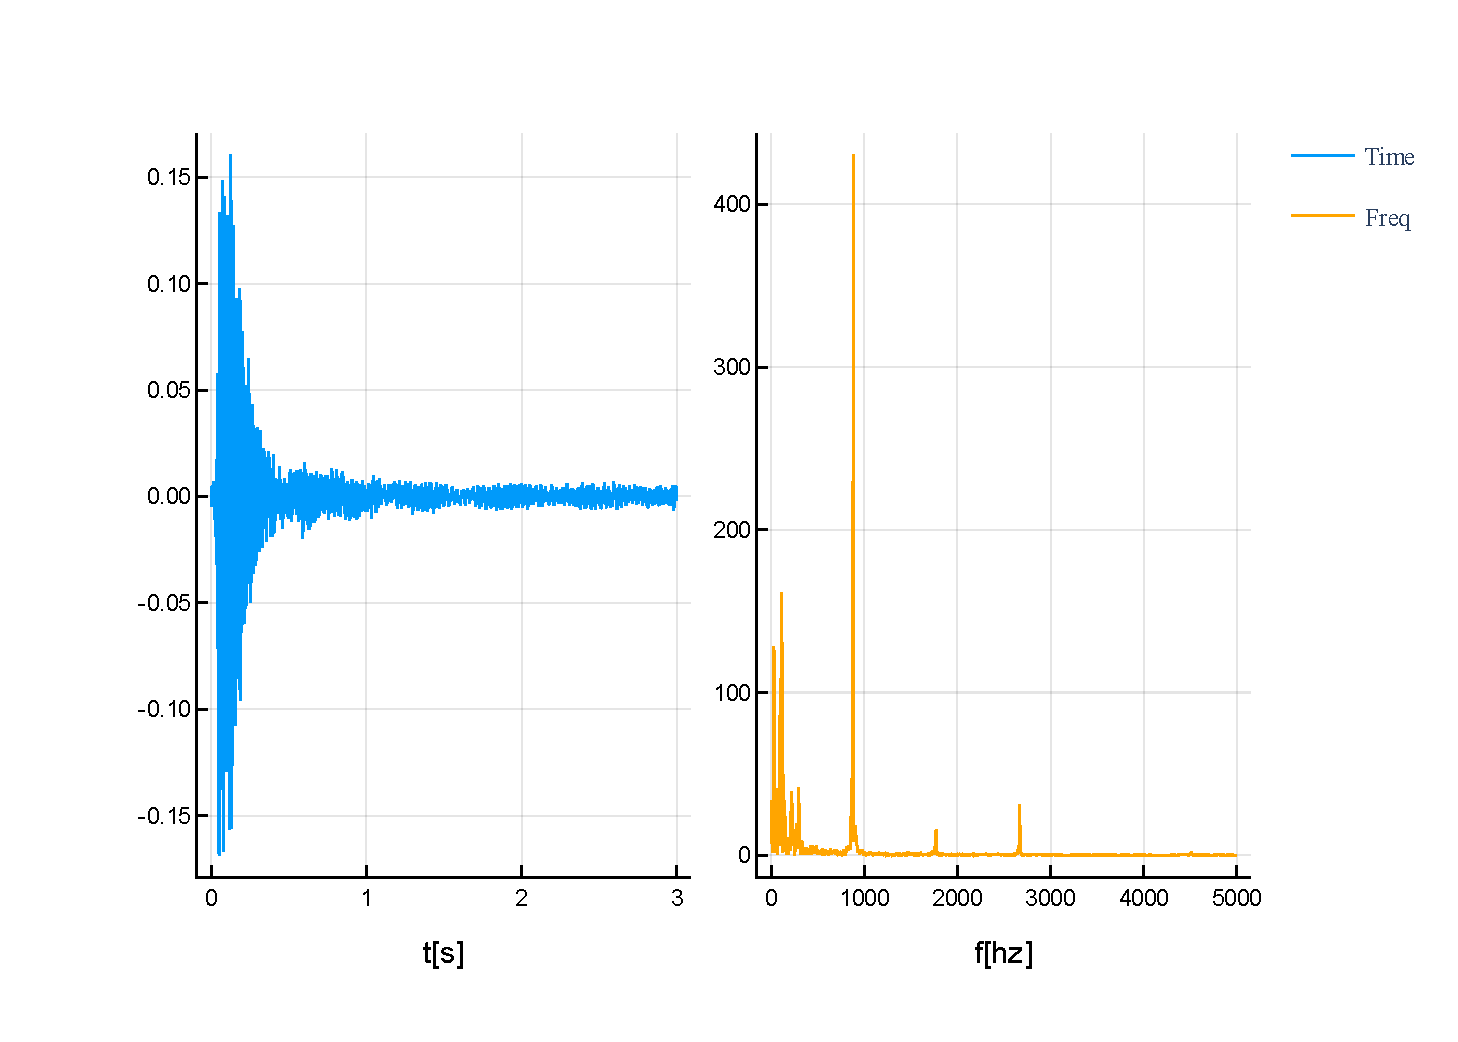
\includegraphics[width=1.0\linewidth]{assets/A5.pdf}
	\caption{Notas A5 en tiempo y frecuencia}
	\label{fig:espectro}
\end{figure}

\bigskip
El origen de la base de datos es una librería de piano de la compañía \textit{FluffyAudio} \textit{\url{(https://www.fluffyaudio.com/shop/scoringpiano)}} 
grabada en 2016 y pensada para jazz, música clásica y bandas sonoras.

\section{Análisis bibliográfico}
\label{Análisis bibliográfico}
Para profundizar en el tema antes de abordarlo, en esta sección se analizan diferentes artículos científicos relacionados con la inteligencia
artificial y el reconocimiento de audio, ya sea específicamente relacionado o no con el mundo del reconocimiento de piezas o notas musicales.

\bigskip
Trabajos como el de \cite{osmalsky2012neural} nos aportan nuevos enfoques, 
en el que, en lugar de detectar las notas por separado, analizan todo el espectro de frecuencias para poder reconocer acordes completos de diferentes instrumentos;
utilizan una técnica llamada Pitch Class Profile (PCP), que obtiene las relaciones energéticas de cada nota en la escala a partir de un audio.

\bigskip
Además, como resumen \cite{benetos2018automatic},
a pesar del estado avanzado de la transcripción automática de canciones, aún están presentes retos tales como la independencia de los intrumentos, de los estilos
musicales o la interpretación de la expresividad.

\bigskip
Otros trabajos mas antiguos como los de \cite{foo1999recognition}, describen un algoritmo capaz de reconocer notas
de un piano a partir de piezas sintetizadas o acústicas, que son digitalmente muestreadas y transformadas al dominio de frecuencia usando 
la transformada de Q constante a partir de la cual se la aplican diferentes técnicas para identificar las notas.

\bigskip
En un terreno más general, trabajos como el de \cite{chang2017audio}, exploran la identificación de \textit{covers} utilizando
estructuras más novedosas que no desarrollaremos en este trabajo como son las Redes de Neuronas Convolucionales. Las salidas de este
sistema corresponderían con la probabilidad de ser una \textit{cover} (comparándola con la canción original), y se ordenarían por dicha 
probabilidad elaborando un ranking.

\bigskip
También encontramos la tesis de \cite{klapuri2004signal} que propone un sistema capaz de generar una representación 
simbólica a partir de un audio, centrándose en el desarrollo de los algoritmos que pueden ser usados para detectar y observar sonidos harmónicos en señales polifónicas.
Los cuales fueron evaluados aplicandolos en un programa de transcripción de música para piano implementado y simulado en un entorno Matlab.

\bigskip
En el trabajo de \cite{marolt2002neural} destacamos el uso de sistemas conexionistas para la detección de inicio en señales musicales basandose en la combinacion de un banco de filtros auditivos
, un red neuronal pulsante y un perceptron multicapa. Este uso de sistemas conexionistas también es empleado para sistemas de transcripción de musica de piano polifónico, mostrando ciertas ventajas sobre otros métodos debido a su estructura y 
presentándose como una alternativa viable a los algoritmos ya existentes

\bigskip
El uso de redes de neuronas artificiales también están presentes en trabajos como \cite{solanki2019music}, que aborda la identificación de
los instrumentos que forman part de piezas polifónicas. Utiliza una red de neuronas convolucional de 8 capas y se apoya en los espectrogramas 
MEL para mapear datos del audio.

\bigskip
Para finalizar, ya en un campo algo más alejado del musical, podemos destacar el trabajo elaborado por \cite{baevski2021unsupervised},
el cual profundiza en el campo de reconocimiento del habla mediante inteligencia artificial.
A diferencia de otros sistemas de reconocimiento, este trabajo no usa datos etiquetados que limiten el reconocimiento a un grupo reducido de idiomas. 
Esta técnica necesita menos requerimientos, aprovechando representaciones auto supervisadas del habla para segmentar el audio y aprender a 
mapear desde estas representaciones a fonemas via \textit{Adversarial Training}.

\bigskip

\newpage
\section{Desarrollo}
\label{Desarrollo}
Para el desarrollo de este sistema utilizaremos un método basado en aproximaciones, es decir, comenzaremos acotando el problema e iremos aumentando
la complejidad a medida que obtenemos resultados satisfatorios.

\bigskip
Además, para mejorar la calidad de los experimentos y no depender de la selección aleatoria del conjunto de test y de entrenamiento, utilizaremos
la técnica de \textit{cross validation} (validación cruzada). Esta técnica consiste en repetir y calcular la media aritmética obtenida de las medidas de la evaluación 
sobre k \textit{folds} (conjuntos) distintos.

En concreto, se realizará un \textit{cross validation} con 10 \textit{folds}. El valor del F1-Score y de la precisión
del modelo será el promedio de dichos valores obtenidos en los \textit{folds}.

\subsection{Primera aproximación}
\label{Primera aproximación}

\subsubsection{Descripción}
En esta primera aproximación nos limitaremos a diferenciar únicamente entre dos notas. 
Escogimos las notas \textit{C4} y \textit{A5} de los cuales usaremos 92 y 56 audios de cada una, respectivamente, en total
se utilizarán 148 patrones. En las Figuras \ref{fig:c4} y \ref{fig:a5} podemos ver a la izquierda la señal en tiempo y, a la derecha,
la señal en el dominio de la frecuencia.

\begin{figure}[!ht]
	\centering
	\begin{subfigure}{.5\textwidth}
		\centering
		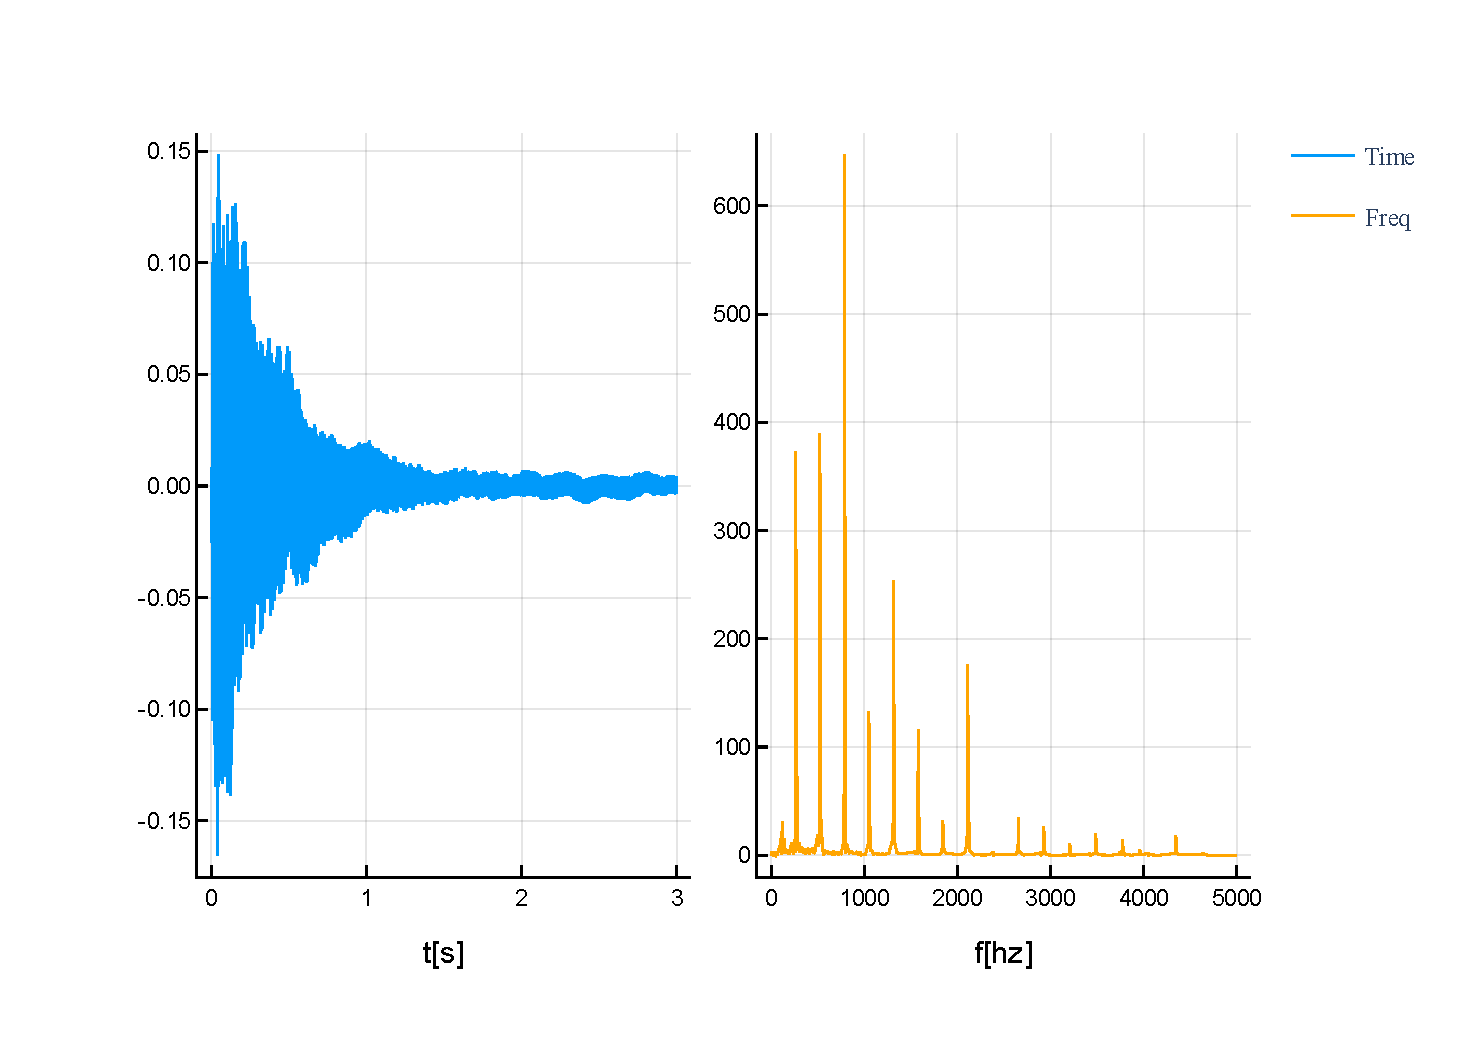
\includegraphics[width=1.0\linewidth]{assets/C4.pdf}
		\caption{C4}
		\label{fig:c4}
	\end{subfigure}%
	\begin{subfigure}{.5\textwidth}
		\centering
		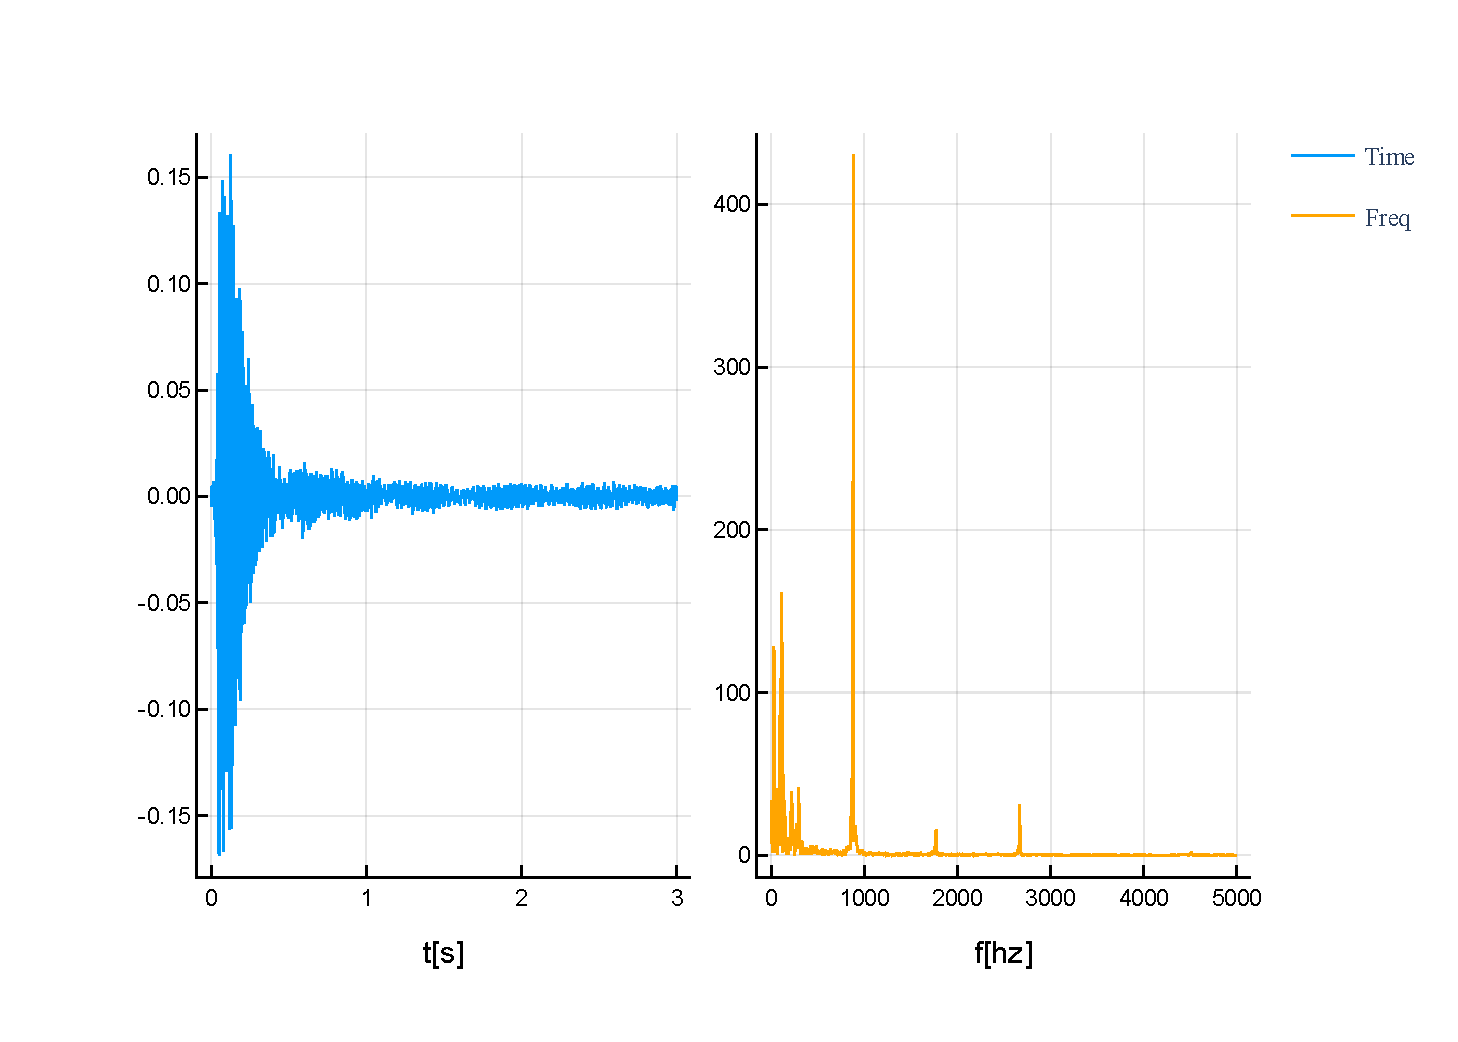
\includegraphics[width=1.0\linewidth]{assets/A5.pdf}
		\caption{A5}
		\label{fig:a5}
	\end{subfigure}
	\caption{Notas en tiempo y frecuencia}
\end{figure}

\bigskip
Dado que cada muestra tiene una duración diferente, decidimos quedarnos solo con los 3 primeros segundos de cada audio (que es donde está la información más
relevante de la nota) y, para la frecuencia, acotaremos cada señal entre 0 y 5000 Hz. Ya que la frecuencia máxima que se alcanza en el 
piano clásico es de 4186 Hz (\textit{C8}) y la más baja, en nuestra base de datos, es de 32.7Hz (\textit{C1}), escogimos un rango
de frecuncias ampliado debido a que es posible que exista información que nos ayude a identificar la nota.

\bigskip
Además, como las notas de un mismo instrumento se diferencian principalmente por la frecuencia (una nota más aguda tiene una mayor frecuencia
y una más grave, una menor), calcularemos de las señales en el dominio del tiempo su relación en el dominio de la frecuencia utilizando la
Transformada de Fourier y, posteriormente, extraeremos las siguientes características:
\begin{itemize}
	\item \textbf{Energia media de la señal}: ya que las señales con más frecuencia (más agudas) tienen más energía, esta característica nos podría
		ayudar a diferenciar entre notas tocadas con la misma intensidad.
	\item \textbf{Media, desviación tipica, y valor máximo de la intensidad en el dominio de la frecuencia, en intervalos no uniformes}: la frecuencia de cada nota
		aumenta de forma exponencial siguiendo la fórmula:

		\begin{equation}
			f_{i+1} = f_{i}\cdot(\sqrt[12]{2}), f_0 = 27.5 Hz
		\end{equation}

		Por ello decidimos dividir el espectro en \textbf{10 intervalos} de longitud variable siguiendo dicha distribución. 
		Podríamos entonces obtener un intervalo donde la media y la desviación típica de la frecuencia fueran más elevados que el resto,
		ayudándonos a identificar la nota.
		
		Los intervalos que usaremos son los siguientes:
		
		\textit{(0.0, 380.3), (380.3, 783.21), (783.21, 1210.08), (1210.08, 1662.33),\newline
		(1662.33, 2141.47), (2141.47, 2649.11), (2649.11, 3186.93), (3186.93, 3756.73), 
		(3756.73, 4360.42) y (4360.42, 5000.0)}
	\item \textbf{Zero-crossing/s}: esta característica determina las veces que la señal, en el dominio del tiempo, toma el valor 0 por segundo.
		Como dicha cracterística nos proporcionaría valores similares a la frecuencia media de la señal, podría contribuír a su correcta clasificación.
\end{itemize}

\bigskip
En lo referente al preprocesado de los datos, hemos decidido optar por una \textbf{normalización de media cero},
debido a que los datos no están acotados en un intervalo y pueden tomar cualquier valor, ya sea
en tiempo o en frecuencia.
Aunque las frecuencias de las notas sí que están acotadas en un intervalo, en la señal
puede haber ruido que sobrepase los valores típicos, por lo que una normalización entre mínimo y máximo no sería lo adecuado.

Así, obtuvimos para cada característica, la media y la desviación típica. Se muestran dichos datos en la Tabla \ref{Tab:Features_1}.

\newpage

\begin{table}[!ht]
	\caption{Parámetros de normalización para cada característica}
	\centering
		\begin{tabular}{||c c c||}
			\hline
			Característica & Media & Desviación Típica  \\ [0.5ex]
			\hline\hline
			E & $0.0045678928$ & $0.0035726614$ \\
			\hline
			zero-crossing & $1797.2139$ & $1352.7441$ \\
			\hline
			m\textsubscript{1} & $16.821161$ & $11.616611$ \\
			\hline
			m\textsubscript{2} & $9.4079$ & $5.8349323$ \\
			\hline
			m\textsubscript{3} & $14.607474$ & $11.515968$ \\
			\hline
			m\textsubscript{4} & $3.8720663$ & $3.5469663$ \\
			\hline
			m\textsubscript{5} & $2.3520973$ & $2.1539617$ \\
			\hline
			m\textsubscript{6} & $0.48698702$ & $0.6487291$ \\
			\hline
			m\textsubscript{7} & $0.7153551$ & $1.0973071$ \\
			\hline
			m\textsubscript{8} & $0.40077275$ & $0.500489$ \\
			\hline
			m\textsubscript{9} & $0.22367951$ & $0.3412378$ \\
			\hline
			m\textsubscript{10} & $0.23234393$ & $0.5112222$ \\
			\hline
			std\textsubscript{1} & $54.282375$ & $46.679535$ \\
			\hline
			std\textsubscript{2} & $31.582827$ & $27.185955$ \\
			\hline
			std\textsubscript{3} & $57.896194$ & $38.439426$ \\
			\hline
			std\textsubscript{4} & $11.108885$ & $12.696077$ \\
			\hline
			std\textsubscript{5} & $7.0041313$ & $6.732649$ \\
			\hline
			std\textsubscript{6} & $0.52131796$ & $0.72755563$ \\
			\hline
			std\textsubscript{7} & $2.7318008$ & $4.6750984$ \\
			\hline
			std\textsubscript{8} & $0.9234557$ & $1.2807367$ \\
			\hline
			std\textsubscript{9} & $0.47755784$ & $0.89846444$ \\
			\hline
			std\textsubscript{10} & $0.5695597$ & $1.2890217$ \\
			\hline
			max\textsubscript{1} & $832.8222$ & $779.30615$ \\
			\hline
			max\textsubscript{2} & $567.7255$ & $505.1785$ \\
			\hline
			max\textsubscript{3} & $901.9232$ & $548.2265$ \\
			\hline
			max\textsubscript{4} & $192.80989$ & $237.47154$ \\
			\hline
			max\textsubscript{5} & $98.938354$ & $103.55783$ \\
			\hline
			max\textsubscript{6} & $4.392064$ & $6.0777674$ \\
			\hline
			max\textsubscript{7} & $40.596066$ & $65.99385$ \\
			\hline
			max\textsubscript{8} & $11.672165$ & $15.524432$ \\
			\hline
			max\textsubscript{9} & $5.7904434$ & $10.440257$ \\
			\hline
			max\textsubscript{10} & $5.6131926$ & $11.565159$ \\
			\hline
		\end{tabular}
	\label{Tab:Features_1}
\end{table}
Donde:
\begin{itemize}
	\item \textit{E} indica la \textbf{energía de la señal}.
	\item \textit{m\textsubscript{i}} indica la \textbf{media de la intensidad} en el intervalo \textit{i} en frecuencia.
	\item \textit{std\textsubscript{i}} indica la \textbf{desviación típica de la intensidad} en el intervalo \textit{i} en frecuencia.
	\item \textit{max\textsubscript{i}} indica el \textbf{máximo de la intensidad} en el intervalo \textit{i} en frecuencia.
\end{itemize}	

\newpage
Como el entrenamiento de una RNA es un proceso no determinista, en cada \textit{fold}
tendremos que entrenar la RNA varias veces, y promediar los resultados. Para estos experimentos,
se ha repetido 30 veces el entrenamiento de la RNA en cada \textit{fold}, devolviendo el resultado promedio de esas 30 ejecuciones.

\bigskip
Para poder evaluar el modelo con mejor rendimiento, como ya se ha dicho antes, utilizaremos como medida el promedio
del \textbf{F1-Score} en los \textit{folds}. Si hay empate en dicha media, se elegirá el modelo con menor
desviación típica de la métrica.

\subsubsection{Resultados}
Para permitir la reproducibilidad de los experimentos, se utilizó \textit{100} como semilla de generación de números
aleatorios.

\paragraph{RNA}

Para el entrenamiento de las RNA, se han utilizado los siguientes parámetros en común:
\begin{itemize}
	\item Ratio de aprendizaje: $0.01$
	\item Ratio de patrones para el conjunto de validación: $0.2$.
	\item Máximo número de ciclos (\textit{epochs}) de entrenamiento: $1500$.
	\item Máximo número de ciclos (\textit{epochs}) de entrenamiento sin mejorar el error de validación: $5$.
	\item Algoritmo de optimización: ADAM.
	\item Función de \textit{loss}: \textit{Binary Cross Entropy}.
\end{itemize}

El hiperparámetro que hemos variado ha sido la arquitectura de neuronas a utilizar.
Utilizamos 8 arquitecturas distintas,
donde la arquitectura [$i$] denota una RNA con una única capa oculta con $i$ neuronas y la arquitectura [$i$, $j$] 
denota una neurona con dos capas ocultas; con $i$ neuronas en la primera capa oculta y $j$ neuronas en la segunda capa oculta.

Se muestran los resultados de la experimentación en la Tabla \ref{Tab:ANN_1}.

\begin{table}[ht]
	\caption{Resultados RNA}
	\centering
		 \begin{tabular}{||c c c||}
			 \hline
			 Arquitectura & F1-Score & Precisión  \\ [0.5ex]
			 \hline\hline
			 [2] & $1.0 \pm 0.0$ & $1.0 \pm 0.0$ \\
			 \hline
			 [4] & $1.0 \pm 0.0$ & $1.0 \pm 0.0$ \\
			 \hline
			 [8] & $1.0 \pm 0.0$ & $1.0 \pm 0.0$ \\
			 \hline
			 [2, 4] & $0.9119 \pm 0.12531$ & $0.96487 \pm 0.05054$ \\
			 \hline
			 [2, 8] & $0.90667 \pm 0.14724$ & $0.96524 \pm 0.05412$ \\
			 \hline
			 [4, 2] & $1.0 \pm 0.0$ & $1.0 \pm 0.0$ \\
			 \hline
			 [4, 4] & $0.99 \pm 0.0225$ & $0.99643 \pm 0.00804$ \\
			 \hline
			 [4, 8] & $0.9621 \pm 0.0974$ & $0.97934 \pm 0.05699$ \\
			 \hline
		 \end{tabular}
	\label{Tab:ANN_1}
\end{table}

\paragraph{SVM}

Para las máquinas de soporte vectorial hemos utilizado 8 configuraciones distintas de los hiperparámetros de \textit{kernel},
grado del \textit{kernel} (sólo se utiliza en \textit{kernel} polinomial), \textit{gamma} y \textit{C}.

Se muestran los resultados de la experimentación en la Tabla \ref{Tab:SVM_1}.

\begin{table}[!ht]
	\caption{Resultados SVM}
	\centering
		\begin{tabular}{||c c c||}
			\hline
			(kernel, grado, gamma, C) & F1-Score & Precisión  \\ [0.5ex]
			\hline\hline
			(poly, $3$, $1$, $1$) & $1.0 \pm 0.0$ & $1.0 \pm 0.0$ \\
			\hline
			(rbf, $3$, $1$, $1$) & $0.93642 \pm 0.07368$ & $0.94119 \pm 0.07166$ \\
			\hline
			(sigmoid, $3$, $1$, $1$) & $0.71875 \pm 0.15823$ & $0.77143 \pm 0.11289$ \\
			\hline
			(poly, $5$, $10$, $0.1$) & $0.99 \pm 0.03162$ & $0.98571 \pm 0.04518$ \\
			\hline
			(rbf, $3$, $10$, $0.1$) & $0.76689 \pm 0.01542$ & $0.62214 \pm 0.02026$ \\
			\hline
			(sigmoid, $3$, $10$, $0.1$) & $0.70059 \pm 0.1406$ & $0.77768 \pm 0.06262$ \\
			\hline
			(rbf, $3$, $0.01$, $100$) & $1.0 \pm 0.0$ & $1.0 \pm 0.0$ \\
			\hline
			(rbf, $3$, $100$, $0.01$) & $0.76689 \pm 0.01542$ & $0.62214 \pm 0.02026$ \\
			\hline
		\end{tabular}
	\label{Tab:SVM_1}
\end{table}

\paragraph{Árboles de decisión}
Para los árboles de decisión hemos utilizado 6 configuraciones distintas del hiperparámetro de profundidad máxima.

Se muestran los resultados de la experimentación en la Tabla \ref{Tab:DecisionTree_1}.

\begin{table}[!ht]
	\caption{Resultados Árbol de decisión}
	\centering
		 \begin{tabular}{||c c c||}
			 \hline
			 Altura máxima & F1-Score & Precisión  \\ [0.5ex]
			 \hline\hline
			 $2$ & $1.0 \pm 0.0$ & $1.0 \pm 0.0$ \\
			 \hline
			 $4$ & $1.0 \pm 0.0$ & $1.0 \pm 0.0$ \\
			 \hline
			 $8$ & $1.0 \pm 0.0$ & $1.0 \pm 0.0$ \\
			 \hline
			 $16$ & $1.0 \pm 0.0$ & $1.0 \pm 0.0$ \\
			 \hline
			 $32$ & $1.0 \pm 0.0$ & $1.0 \pm 0.0$ \\
			 \hline
			 $64$ & $1.0 \pm 0.0$ & $1.0 \pm 0.0$ \\
			 \hline
		 \end{tabular}
	\label{Tab:DecisionTree_1}
\end{table}

\paragraph{kNN}
Para el modelo kNN hemos utilizado 6 configuraciones distintas del hiperparámetro de k (número de vecinos más cercanos).

Se muestran los resultados de la experimentación en la Tabla \ref{Tab:kNN_1}.

\begin{table}[!ht]
	\caption{Resultados kNN}
	\centering
		 \begin{tabular}{||c c c||}
			 \hline
			 K & F1-Score & Precisión  \\ [0.5ex]
			 \hline\hline
			 $2$ & $1.0 \pm 0.0$ & $1.0 \pm 0.0$ \\
			 \hline
			 $3$ & $1.0 \pm 0.0$ & $1.0 \pm 0.0$ \\
			 \hline
			 $5$ & $1.0 \pm 0.0$ & $1.0 \pm 0.0$ \\
			 \hline
			 $8$ & $1.0 \pm 0.0$ & $1.0 \pm 0.0$ \\
			 \hline
			 $13$ & $1.0 \pm 0.0$ & $1.0 \pm 0.0$ \\
			 \hline
			 $21$ & $0.99091 \pm 0.02875$ & $0.99286 \pm 0.02259$ \\
			 \hline
		 \end{tabular}
	\label{Tab:kNN_1}
\end{table}

\subsubsection{Discusión}
Los resultados han sido muy buenos, ya que en la mayoría de casos se alcanza una \textbf{precisión} y un \textbf{F1-Score} del 100\% o muy alto. 

\bigskip
En general, los sistemas se equivocan en muy pocos patrones. Esto se puede deber a que el problema elegido en esta aproximación
era excesivamente sencillo para el elevado número de características escogidas, permitiéndonos separar perfectamentes los patrones
en las dos clases.

\bigskip
En lo referente a las características, por una parte estas han sido correctamente elegidas, ya que alcanzamos una precisión muy alta. Pero 
por otra parte, el hecho de que algunos sistemas concretos no 
funcionen tan bien (por ejemplo, algunos SVM), se podría deber al elevado número de características, 
ya que algunas de ellas pueden ser innecesarias o hasta contraproducentes en este sencillo problema. Una buena estrategia sería el intentar 
reducir el número de características en futuras aproximaciones, pero hay que tener cuidado, ya que si aumentamos el número de clases, 
podría darse el caso de haber eliminado una característica necesaria para una correcta clasificación.

En concreto, las características que creemos que son las que producen mejores resultados son las que se refieren a los intervalos 
en frecuencia de \textit{(0.0, 380.3)} y \textit{(783.21, 1210.08)}, debido a que es en ellos donde se sitúan las frecuencia de las notas 
\textit{C4} y \textit{A5}, respectivamente.
Las características que se corresponden a dichos intervalos son \textit{m\textsubscript{1}, std\textsubscript{1}, max\textsubscript{1}}
para el primer intervalo y \textit{m\textsubscript{3}, std\textsubscript{3}, max\textsubscript{3}} para el segundo intervalo.

Otra característica que podría funcionar sería la frecuencia en la que se alcanza el pico absoluto en intensidad de la señal,
o la media de las K frecuencias con mayor intensidad, sin tener en cuenta la división en intervalos. También se podría aumentar
el número de intervalos en los que obtener las características, para poder así separar mejor las notas con frecuencias más cercanas.

\bigskip
Todos los algoritmos tienen al menos una configuración con un \textbf{F1-Score} de $1.0 \pm 0.0$, por lo que es complicado encontrar uno que sea el mejor.

Podemos destacar la RNA con una arquitectura de una única capa oculta con 2 neuronas, ya que es un modelo muy sencillo y podemos esperar que, cuanto
más sencillo sea un modelo, mayor será también su capacidad de generalización. 

\bigskip
En la Figura \ref{fig:rna_train_1} podemos ver un gráfico del entrenamiento de dicha RNA, donde observamos el error
cometido en los conjuntos de test, validación y entrenamiento para cada ciclo de entrenamiento. Este se ha realizado
utilizando todos los patrones, separando un 20\% para el conjunto de test.
Además, se puede ver que se ha producido una parada temprana, ya que el sistema no ha realizado
el máximo número de ciclos de entrenamiento ($1500$ ciclos) y se puede distinguir también como la curva de la gráfica desciende muy rápido. 
Esto se puede deber a que tenemos un ratio de aprendizaje alto para este problema concreto.

\bigskip
En la Tabla \ref{tab:confusion_matrix_1} podemos ver una matriz de confusión para la RNA entrenada anteriormente. Las predicciones se hicieron sobre un conjunto
de test que supone un 20\% de todos los patrones utilizados. El 80\% de los patrones restantes se utilizó para el entrenamiento de la RNA,
ya que el conjunto de entrenamiento no se debería utilizar para realizar predicciones.

\begin{figure}[!ht]
	\centering
	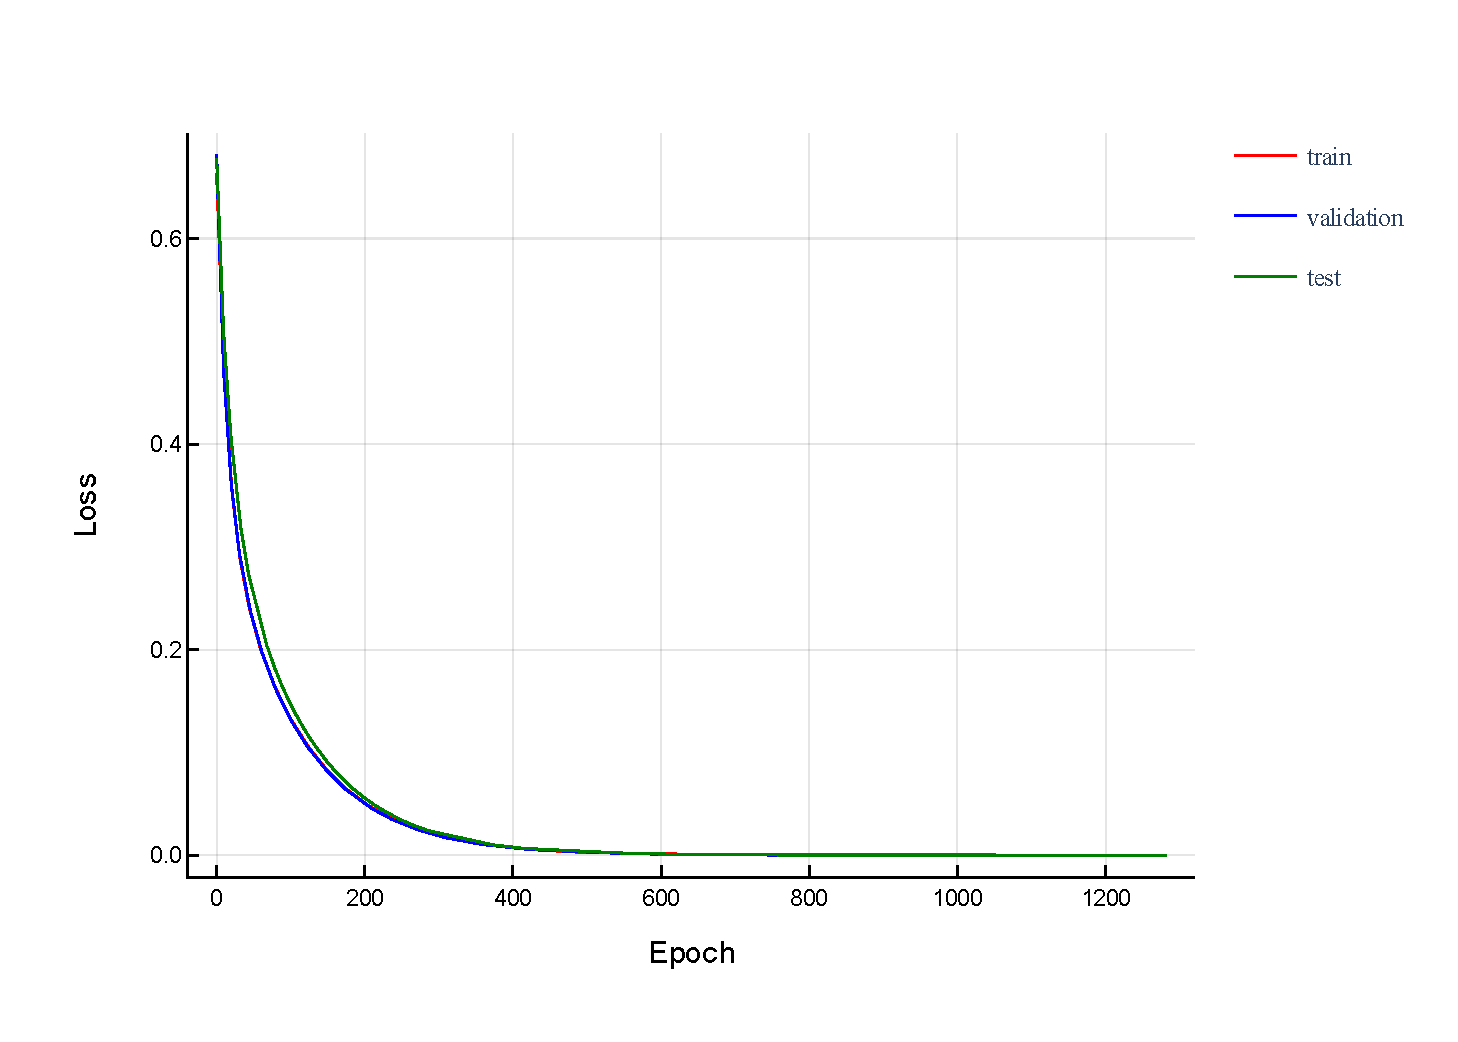
\includegraphics[width=1.0\linewidth]{assets/best_rna_train_1.pdf}
	\caption{Entrenamiento RNA}
	\label{fig:rna_train_1}
\end{figure}

\begin{table}[!ht]
	\centering
	
	\resizebox{5.5cm}{!}{
		\begin{tabular}{cllcllcll}
			\multicolumn{1}{l}{}  &                   &                                          & \multicolumn{6}{c}{Predicc.}                                                        \\
			\multicolumn{1}{l}{}  &                   &                                          & \multicolumn{6}{l}{}                                                                \\
			\multicolumn{1}{l}{}  &                   &                                          & \multicolumn{3}{c}{A5}                   & \multicolumn{3}{c}{C4}                   \\ \cline{4-9} 
			\multirow{6}{*}{Real} & \multirow{6}{*}{} & \multicolumn{1}{c|}{\multirow{3}{*}{A5}} & \multicolumn{3}{c|}{\multirow{3}{*}{15}} & \multicolumn{3}{c|}{\multirow{3}{*}{0}}  \\
								  &                   & \multicolumn{1}{c|}{}                    & \multicolumn{3}{c|}{}                    & \multicolumn{3}{c|}{}                    \\
								  &                   & \multicolumn{1}{c|}{}                    & \multicolumn{3}{c|}{}                    & \multicolumn{3}{c|}{}                    \\ \cline{4-9} 
								  &                   & \multicolumn{1}{l|}{\multirow{3}{*}{C4}} & \multicolumn{3}{c|}{\multirow{3}{*}{0}}  & \multicolumn{3}{c|}{\multirow{3}{*}{15}} \\
								  &                   & \multicolumn{1}{l|}{}                    & \multicolumn{3}{c|}{}                    & \multicolumn{3}{c|}{}                    \\
								  &                   & \multicolumn{1}{l|}{}                    & \multicolumn{3}{c|}{}                    & \multicolumn{3}{c|}{}                    \\ \cline{4-9} 
			\end{tabular}
	
	}
	\caption{Matriz de confusión RNA}
    \label{tab:confusion_matrix_1}
\end{table}

\newpage
Pero aunque se alcance ya un buen resultado con un modelo sencillo como puede ser la RNA anterior, caben destacar los árboles de decisión,
que son modelos que pueden ofrecer explicabilidad sobre sus predicciones, además de presentar un entrenamiento determinista, por lo que 
si tenemos que elegir el mejor modelo, nos decantaríamos por este (en concreto, el de altura máxima de 2, ya que es el más sencillo), 
ya que presenta también un 100\% de \textbf{F1-Score}.

\bigskip
Aunque si deseamos un modelo con una base matemática más fuerte, en vez de un modelo con una base estadística como puede ser un árbol de regresión,
utilizar una máquina de soporte vectorial con un \textit{kernel} polinomial de grado 3, y ambos valores de \textit{gamma} y \textit{C} de 1, también sería una buena opción. 

Los algoritmos que han funcionado peor han sido ciertas configuraciones de los SVM, en concreto las que utilizan un \textit{kernel} sigmoidal.
Entonces, utilizar un \textit{kernel} sigmoidal no parece ofrecer buenos resultados para estos patrones.

\newpage
\subsection{Segunda aproximación}
\label{Segunda aproximación}

\subsubsection{Descripción}
Como hemos obtenido resultados muy buenos en la aproximación anterior, aumentaremos la complejidad del problema,
es decir, añadiremos más notas a ser clasificadas. Se clasificarán entonces 15 notas y se dispondrá de 
1090 patrones para ser utilizados por el sistema.

Las notas que vamos a clasificar son: \textit{C1}, \textit{C2}, \textit{C3}, \textit{C4}, \textit{C5}, \textit{C6}, \textit{C7}, \textit{C8}, \textit{A1}, \textit{A2}, \textit{A3}, \textit{A4}, \textit{A5}, \textit{A6} y \textit{A7}.

\bigskip
Se puede ver algunos ejemplos de los \textit{samples} que vamos a utilizar, con su señal en el dominio del tiempo y en el
dominio de la frecuencia, en las Figuras \ref{fig:c3}, \ref{fig:c6}, \ref{fig:a3} y \ref{fig:a6}.

\begin{figure}[!ht]
	\centering
	\begin{subfigure}{.5\textwidth}
		\centering
		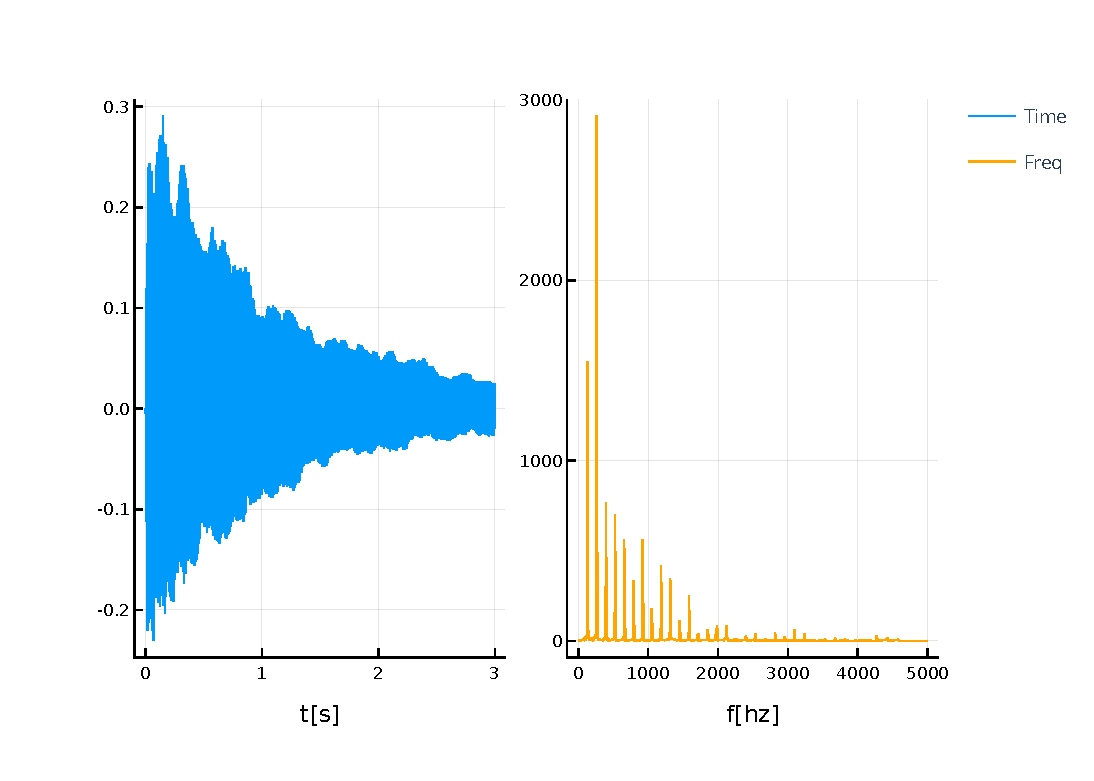
\includegraphics[width=1.0\linewidth]{assets/C3.pdf}
		\caption{C3}
		\label{fig:c3}
	\end{subfigure}%
	\begin{subfigure}{.5\textwidth}
		\centering
		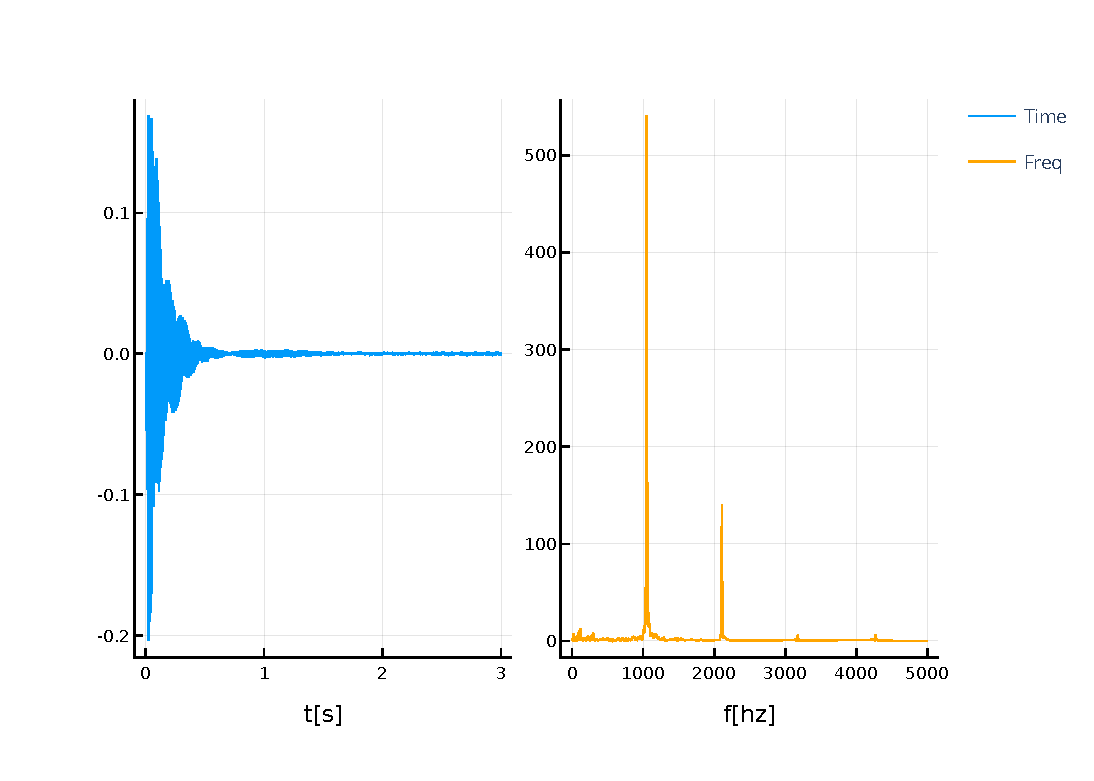
\includegraphics[width=1.0\linewidth]{assets/C6.pdf}
		\caption{A6}
		\label{fig:c6}
	\end{subfigure}
	\caption{}
\end{figure}

\begin{figure}[!ht]
	\centering
	\begin{subfigure}{.5\textwidth}
		\centering
		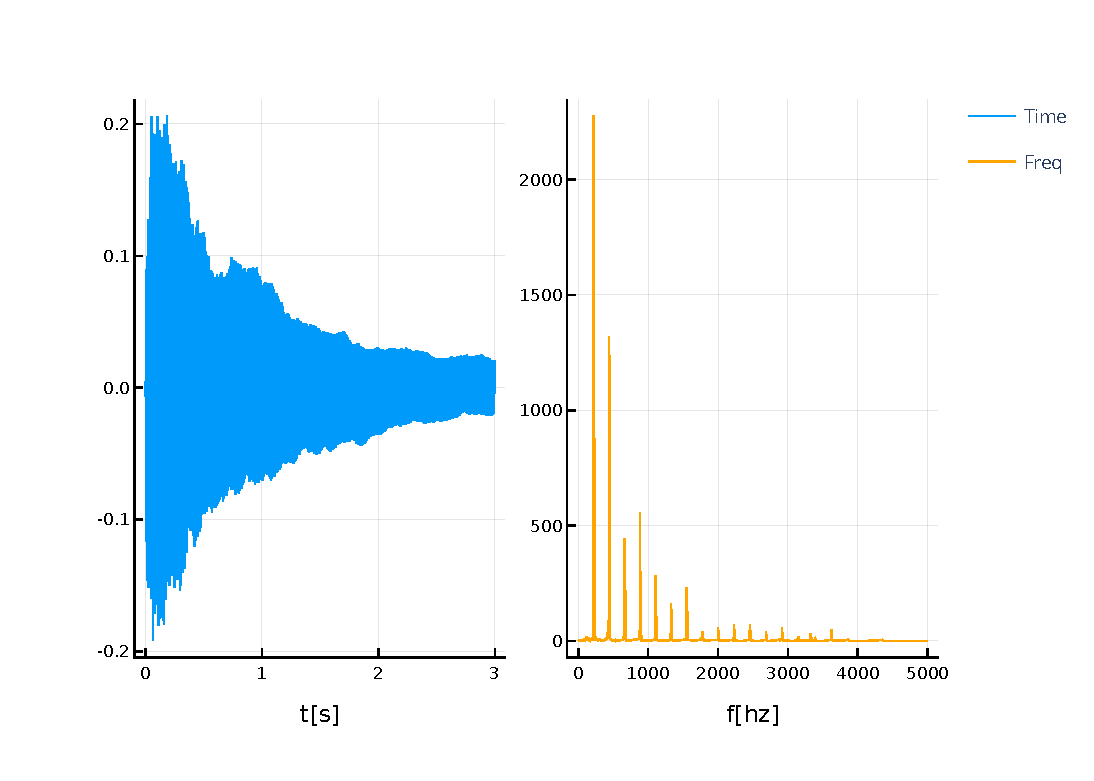
\includegraphics[width=1.0\linewidth]{assets/A3.pdf}
		\caption{A3}
		\label{fig:a3}
	\end{subfigure}%
	\begin{subfigure}{.5\textwidth}
		\centering
		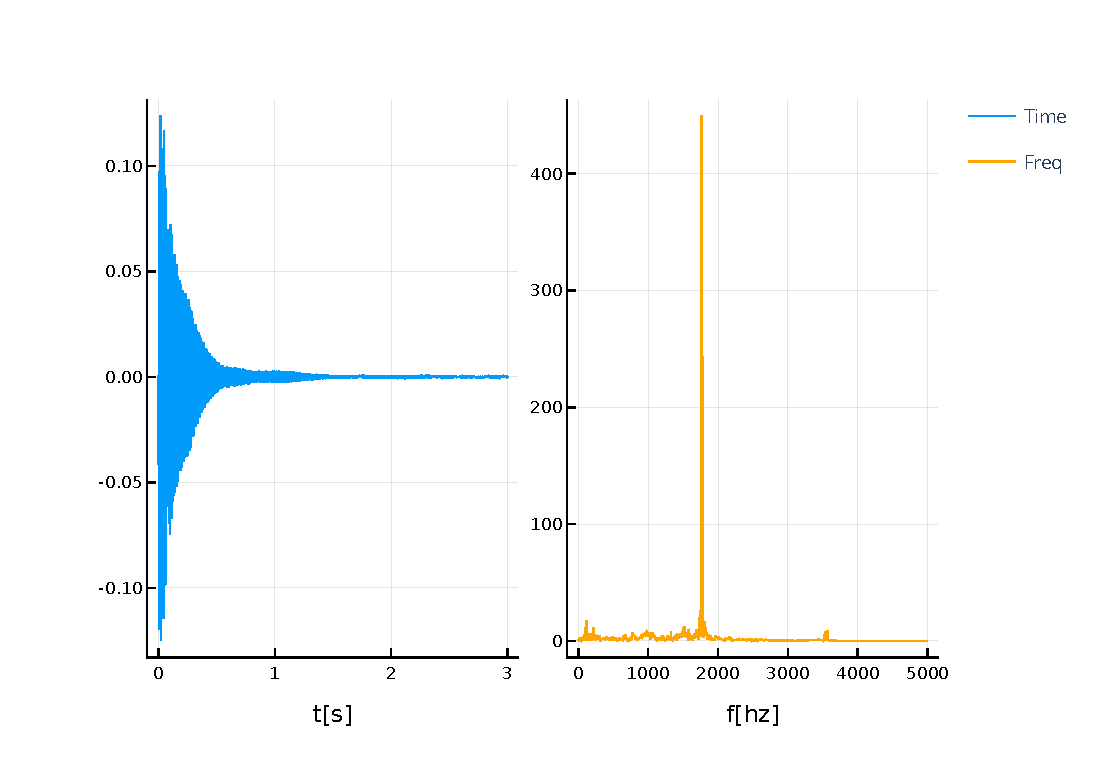
\includegraphics[width=1.0\linewidth]{assets/A6.pdf}
		\caption{A6}
		\label{fig:a6}
	\end{subfigure}
	\caption{}
\end{figure}

\newpage
Como hemos aumentado mucho el número de clases a clasificar, decidimos aumentar también el número de características 
para lograr una correcta diferenciación entre las clases que sean más similares.

En concreto, añadiremos las siguientes características:

\begin{itemize}
	\item \textbf{Frecuencia en la que se alcanza la máxima intensidad} en cada uno de los 10 intervalos
	que ya se especificaron en la aproximación anterior.
\end{itemize}

No se producen cambios sobre las características que fueron incorporadas en la aproximación anterior.

Para el preprocesado de los datos, utilizaremos, como se mencionó en la aproximación anterior,
una normalización de media cero.
Así, obtuvimos para cada característica, la media y la desviación típica. Se muestran dichos datos en las Tablas \ref{Tab:Features_2_1}
y \ref{Tab:Features_2_2}.

\bigskip

\begin{table}[!ht]
	\caption{Parámetros de normalización (I)}
	\centering
		\begin{tabular}{||c c c||}
			\hline
			Característica & Media & Desviación Típica  \\ [0.5ex]
			\hline\hline
			E & $0.0050883736$ & $0.0088912$ \\
			\hline
			zero-crossing & $3743.606$ & $5035.344$ \\
			\hline
			m\textsubscript{1} & $15.578591$ & $18.397396$ \\
			\hline
			m\textsubscript{2} & $11.147778$ & $9.179351$ \\
			\hline
			m\textsubscript{3} & $9.6564455$ & $9.295277$ \\
			\hline
			m\textsubscript{4} & $4.0943613$ & $4.225765$ \\
			\hline
			m\textsubscript{5} & $3.6645029$ & $4.699565$ \\
			\hline
			m\textsubscript{6} & $1.0346977$ & $1.3888823$ \\
			\hline
			m\textsubscript{7} & $0.71540374$ & $1.0062366$ \\
			\hline
			m\textsubscript{8} & $0.68384236$ & $1.307346$ \\
			\hline
			m\textsubscript{9} & $0.38978294$ & $0.8350492$ \\
			\hline
			m\textsubscript{10} & $0.44757652$ & $1.4078437$ \\
			\hline
			std\textsubscript{1} & $49.61187$ & $74.658005$ \\
			\hline
			std\textsubscript{2} & $39.12518$ & $41.206196$ \\
			\hline
			std\textsubscript{3} & $29.023785$ & $34.23634$ \\
			\hline
			std\textsubscript{4} & $8.560635$ & $11.001557$ \\
			\hline
			std\textsubscript{5} & $9.463276$ & $12.920476$ \\
			\hline
			std\textsubscript{6} & $1.5626754$ & $2.6529887$ \\
			\hline
			std\textsubscript{7} & $1.6301519$ & $2.8170295$ \\
			\hline
			std\textsubscript{8} & $1.2500806$ & $2.295387$ \\
			\hline
			std\textsubscript{9} & $0.5342404$ & $0.98041487$ \\
			\hline
			std\textsubscript{10} & $0.7347808$ & $2.2108128$ \\
			\hline
			max\textsubscript{1} & $944.37256$ & $1596.2578$ \\
			\hline
			max\textsubscript{2} & $748.07245$ & $844.44037$ \\
			\hline
			max\textsubscript{3} & $442.8393$ & $524.42633$ \\
			\hline
			max\textsubscript{4} & $130.52594$ & $192.10622$ \\
			\hline
			max\textsubscript{5} & $129.60143$ & $179.40135$ \\
			\hline
			max\textsubscript{6} & $19.159048$ & $36.38486$ \\
			\hline
			max\textsubscript{7} & $22.589241$ & $40.29418$ \\
			\hline
			max\textsubscript{8} & $13.267355$ & $21.899231$ \\
			\hline
			max\textsubscript{9} & $5.3473926$ & $10.327133$ \\
			\hline
			max\textsubscript{10} & $5.520794$ & $13.594501$ \\
			\hline
		\end{tabular}
	\label{Tab:Features_2_1}
\end{table}

\begin{table}[!ht]
	\caption{Parámetros de normalización (II)}
	\centering
		\begin{tabular}{||c c c||}
			\hline
			Característica & Media & Desviación Típica  \\ [0.5ex]
			max-freq\textsubscript{1} & $174.89925$ & $87.058235$ \\
			\hline
			max-freq\textsubscript{2} & $521.6259$ & $125.11409$ \\
			\hline
			max-freq\textsubscript{3} & $961.683$ & $100.904564$ \\
			\hline
			max-freq\textsubscript{4} & $1394.9509$ & $126.07898$ \\
			\hline
			max-freq\textsubscript{5} & $1897.9567$ & $174.84656$ \\
			\hline
			max-freq\textsubscript{6} & $2353.7712$ & $191.61922$ \\
			\hline
			max-freq\textsubscript{7} & $2791.1377$ & $166.82562$ \\
			\hline
			max-freq\textsubscript{8} & $3426.2026$ & $169.13255$ \\
			\hline
			max-freq\textsubscript{9} & $4093.2415$ & $226.97453$ \\
			\hline
			max-freq\textsubscript{10} & $4583.3877$ & $193.1689$ \\
			\hline
		\end{tabular}
	\label{Tab:Features_2_2}
\end{table}

\newpage
\hphantom{skip}
\newpage
Donde:
\begin{itemize}
	\item \textit{E} indica la \textbf{energía de la señal}.
	\item \textit{m\textsubscript{i}} indica la \textbf{media de la intensidad} en el intervalo \textit{i} en frecuencia.
	\item \textit{std\textsubscript{i}} indica la \textbf{desviación típica de la intensidad} en el intervalo \textit{i} en frecuencia.
	\item \textit{max\textsubscript{i}} indica el \textbf{máximo de la intensidad} en el intervalo \textit{i} en frecuencia.
	\item \textit{max-freq\textsubscript{i}} indica la \textbf{frecuencia donde se alcanza el máximo de intensidad} en el intervalo \textit{i} en frecuencia.
\end{itemize}

Para estos experimentos se ha repetido 20 veces el entrenamiento de la RNA en cada \textit{fold}, devolviendo el resultado promedio de esas 20 ejecuciones.

\bigskip
Para poder evaluar el modelo con mejor rendimiento, como ya se ha dicho antes, utilizaremos como medida el promedio
del \textbf{F1-Score} en los \textit{folds}. Si hay empate en dicha media, se elegirá el modelo con menor
desviación típica de la métrica.


\newpage
\subsubsection{Resultados}
Para permitir la reproducibilidad de los experimentos, se utilizó \textit{100} como semilla de generación de números
aleatorios.

\paragraph{RNA}

Para el entrenamiento de las RNA, se han utilizado los siguientes parámetros en común:
\begin{itemize}
	\item Ratio de aprendizaje: $0.01$
	\item Ratio de patrones para el conjunto de validación: $0.2$.
	\item Máximo número de ciclos (\textit{epochs}) de entrenamiento: $1500$.
	\item Máximo número de ciclos (\textit{epochs}) de entrenamiento sin mejorar el error de validación: $5$.
	\item Algoritmo de optimización: ADAM.
	\item Función de \textit{loss}: \textit{Cross Entropy}.
\end{itemize}
El hiperparámetro que hemos variado ha sido la arquitectura de neuronas a utilizar. Utilizamos 8 arquitecturas distintas,
donde la arquitectura [$i$] denota una RNA con una única capa oculta con $i$ neuronas y la arquitectura [$i$, $j$] 
denota una neurona con dos capas ocultas; con $i$ neuronas en la primera capa oculta y $j$ neuronas en la segunda capa oculta.

Se muestran los resultados de la experimentación en la Tabla \ref{Tab:ANN_2}

\begin{table}[!ht]
	\caption{Resultados RNA}
	\centering
		 \begin{tabular}{||c c c||}
			 \hline
			 Arquitectura & F1-Score & Precisión  \\ [0.5ex]
			 \hline\hline
			 [8] & $0.92977 \pm 0.01923$ & $0.95523 \pm 0.0131$ \\
			 \hline
			 [16] & $0.96092 \pm 0.0163$ & $0.97591 \pm 0.0112$ \\
			 \hline
			 [32] & $0.96305 \pm 0.01805$ & $0.97745 \pm 0.01137$ \\
			 \hline
			 [8, 8] & $0.87808 \pm 0.01593$ & $0.92368 \pm 0.00628$ \\
			 \hline
			 [16, 4] & $0.76012 \pm 0.03119$ & $0.8518 \pm 0.0233$ \\
			 \hline
			 [16, 8] & $0.92264 \pm 0.02515$ & $0.95168 \pm 0.01708$ \\
			 \hline
			 [32, 16] & $0.9506 \pm 0.01989$ & $0.97044 \pm 0.01033$ \\
			 \hline
			 [32, 32] & $0.95122 \pm 0.02256$ & $0.97004 \pm 0.013$ \\
			 \hline
		 \end{tabular}
	\label{Tab:ANN_2}
	\end{table}

\paragraph{SVM}

Para las máquinas de soporte vectorial hemos utilizado 8 configuraciones distintas de los hiperparámetros de \textit{kernel},
grado del \textit{kernel} (sólo se utiliza en \textit{kernel} polinomial), \textit{gamma} y \textit{C}.

Se muestran los resultados de la experimentación en la Tabla \ref{Tab:SVM_2}

\begin{table}[!ht]
	\caption{Resultados SVM}
	\centering
		 \begin{tabular}{||c c c||}
			 \hline
			 (kernel, grado, gamma, C) & F1-Score & Precisión  \\ [0.5ex]
			 \hline\hline
			 (poly, $3$, $1$, $1$) & $0.97261 \pm 0.02358$ & $0.98158 \pm 0.01438$ \\
			 \hline
			 (rbf, $3$, $1$, $1$) & $0.67559 \pm 0.04297$ & $0.69947 \pm 0.05196$ \\
			 \hline
			 (sigmoid, $3$, $1$, $1$) & $0.28516 \pm 0.03747$ & $0.3575 \pm 0.03929$ \\
			 \hline
			 (poly, $3$, $10$, $0.1$) & $0.97619 \pm 0.02456$ & $0.98415 \pm 0.01345$ \\
			 \hline
			 (rbf, $3$, $10$, $0.1$) & $0.01607 \pm 0.00059$ & $0.13703 \pm 0.00568$ \\
			 \hline
			 (sigmoid, $3$, $10$, $0.1$) & $0.23652 \pm 0.03974$ & $0.33481 \pm 0.04109$ \\
			 \hline
			 (rbf, $3$, $0.01$, $100$) & $0.97415 \pm 0.02285$ & $0.98444 \pm 0.0122$ \\
			 \hline
			 (poly, $3$, $100$, $0.001$) & $0.9678 \pm 0.03578$ & $0.97987 \pm 0.01547$ \\
			 \hline
		 \end{tabular}
	\label{Tab:SVM_2}
	\end{table}

\paragraph{Árboles de decisión}
Para los árboles de decisión hemos utilizado 6 configuraciones distintas del hiperparámetro de profundidad máxima.

Se muestran los resultados de la experimentación en la Tabla \ref{Tab:DecisionTree_2}

\begin{table}[!ht]
	\caption{Resultados Árbol de decisión}
	\centering
		 \begin{tabular}{||c c c||}
			 \hline
			 Altura máxima & F1-Score & Precisión  \\ [0.5ex]
			 \hline\hline
			 $4$ & $0.44767 \pm 0.00668$ & $0.66703 \pm 0.01287$ \\
			 \hline
			 $8$ & $0.86809 \pm 0.02258$ & $0.92653 \pm 0.01909$ \\
			 \hline
			 $16$ & $0.96505 \pm 0.02104$ & $0.9725 \pm 0.0143$ \\
			 \hline
			 $32$ & $0.96786 \pm 0.01849$ & $0.97302 \pm 0.01609$ \\
			 \hline
			 $64$ & $0.97438 \pm 0.01244$ & $0.97779 \pm 0.0102$ \\
			 \hline
			 $128$ & $0.97415 \pm 0.0161$ & $0.9779 \pm 0.01186$ \\
			 \hline
			 $256$ & $0.9672 \pm 0.02388$ & $0.97452 \pm 0.0172$ \\
			 \hline
		 \end{tabular}
	\label{Tab:DecisionTree_2}
	\end{table}

\paragraph{kNN}
Para el modelo kNN hemos utilizado 6 configuraciones distintas del hiperparámetro de k (número de vecinos más cercanos).

Se muestran los resultados de la experimentación en la tabla \ref{Tab:kNN_2}

\begin{table}[!ht]
	\caption{Resultados kNN}
	\centering
		 \begin{tabular}{||c c c||}
			 \hline
			 K & F1-Score & Precisión  \\ [0.5ex]
			 \hline\hline
			 $2$ & $0.95086 \pm 0.01526$ & $0.97073 \pm 0.0088$ \\
			 \hline
			 $3$ & $0.9323 \pm 0.03125$ & $0.95942 \pm 0.0156$ \\
			 \hline
			 $5$ & $0.90323 \pm 0.03494$ & $0.94503 \pm 0.01712$ \\
			 \hline
			 $8$ & $0.86641 \pm 0.03906$ & $0.93135 \pm 0.0199$ \\
			 \hline
			 $13$ & $0.84065 \pm 0.02462$ & $0.90985 \pm 0.01911$ \\
			 \hline
			 $21$ & $0.80344 \pm 0.03804$ & $0.88737 \pm 0.02667$ \\
			 \hline
		 \end{tabular}
	\label{Tab:kNN_2}
\end{table}

\newpage
\subsubsection{Discusión}

En general los resultados son muy buenos, ya que hay varios modelos con un alto F1-Score.
El modelo que mejor funciona es un SVM con función de \textit{kernel} polinomial de grado 3, con
un \textit{gamma} y \textit{C} de $10$ y $0.1$, respectivamente.

Este modelo tiene un F1-Score de $0.97619 \pm 0.02456$, con una precisión de $0.98415 \pm 0.01345$ en los \textit{folds}.
De este resultado podemos concluír que nuestro sistema funciona muy bien, ya que clasificar 15 notas es un problema
relativamente complejo.

\bigskip
Cabe destacar modelos como la RNA con una única capa oculta de $32$ neuronas; el SVM con \textit{kernel} de base radial,
con los parámetros de \textit{gamma} $0.01$ y de \textit{C} $100$; un árbol de decisión con altura máxima de $64$; y
un modelo kNN con un k de $2$. Estos modelos también presentan muy buenos resultados, aunque no los mejores.

El modelo con peor rendimiento es un SVM con kernel de base radial con \textit{gamma} y \textit{C} de
$10$ y $0.1$, respectivamente. Esta configuración del modelo un \textit{F1-Score} de tan solo $0.01607 \pm 0.00059$, 
desconociendo realmente a qué se debe realmente este tan bajo resultado.

\bigskip
En cuanto a las características, creemos que fue un acierto añadir la frecuencia a la que se encuentra el pico de intensidad
en cada intervalo, ya que es una característica muy representativa de la señal y que sirve para diferenciar mejor las notas.
Sin estas nuevas características (y habiendo hecho las pruebas), los resultados no serían tan buenos.

\bigskip
El problema que podemos observar en la matriz de confusión (Tabla \ref{tab:confusion_matrix_2}) para el mejor sistema es que el sistema se equivoca
en las notas más cercanas, como pueden ser \textit{A1}, \textit{A2}, \textit{C1} y \textit{C2}; notas que tienen una frecuencia muy similar y se encuentran
en el primer intervalo, \textit{(0.0, 380.3)}. 

\bigskip
Para poder diferenciar mejor entre estas notas (y entre futuras notas
que puedan ser similares entre ellas), sería una buena opción que se aumentase el número de intervalos a dividir
las frecuencias, para así poder diferenciar de mejor manera dichas notas.

\begin{table}[!ht]
	\centering
	
	\resizebox{15cm}{!}{
		\begin{tabular}{cccccccccccccccccc}
			&                         & \multicolumn{15}{c}{Predicc.}                                                                                                                                                                                                                                                                                                                                                                   &  \\
			&                         & C1                     & C2                     & C3                     & C4                      & C5                      & C6                      & C7                      & C8                      & A1                      & A2                      & A3                      & A4                      & A5                      & A6                      & A7                     &  \\ \cline{3-17}
			  \multirow{15}{*}{Real} & \multicolumn{1}{c|}{C1} & \multicolumn{1}{c|}{3} & \multicolumn{1}{c|}{0} & \multicolumn{1}{c|}{0} & \multicolumn{1}{c|}{0}  & \multicolumn{1}{c|}{0}  & \multicolumn{1}{c|}{0}  & \multicolumn{1}{c|}{0}  & \multicolumn{1}{c|}{0}  & \multicolumn{1}{c|}{1}  & \multicolumn{1}{c|}{0}  & \multicolumn{1}{c|}{0}  & \multicolumn{1}{c|}{0}  & \multicolumn{1}{c|}{0}  & \multicolumn{1}{c|}{0}  & \multicolumn{1}{c|}{0} &  \\ \cline{3-17}
			& \multicolumn{1}{c|}{C2} & \multicolumn{1}{c|}{1} & \multicolumn{1}{c|}{6} & \multicolumn{1}{c|}{1} & \multicolumn{1}{c|}{0}  & \multicolumn{1}{c|}{0}  & \multicolumn{1}{c|}{0}  & \multicolumn{1}{c|}{0}  & \multicolumn{1}{c|}{0}  & \multicolumn{1}{c|}{0}  & \multicolumn{1}{c|}{0}  & \multicolumn{1}{c|}{0}  & \multicolumn{1}{c|}{0}  & \multicolumn{1}{c|}{0}  & \multicolumn{1}{c|}{0}  & \multicolumn{1}{c|}{0} &  \\ \cline{3-17}
			& \multicolumn{1}{c|}{C3} & \multicolumn{1}{c|}{0} & \multicolumn{1}{c|}{0} & \multicolumn{1}{c|}{9} & \multicolumn{1}{c|}{0}  & \multicolumn{1}{c|}{0}  & \multicolumn{1}{c|}{0}  & \multicolumn{1}{c|}{0}  & \multicolumn{1}{c|}{0}  & \multicolumn{1}{c|}{0}  & \multicolumn{1}{c|}{0}  & \multicolumn{1}{c|}{0}  & \multicolumn{1}{c|}{0}  & \multicolumn{1}{c|}{0}  & \multicolumn{1}{c|}{0}  & \multicolumn{1}{c|}{0} &  \\ \cline{3-17}
			& \multicolumn{1}{c|}{C4} & \multicolumn{1}{c|}{0} & \multicolumn{1}{c|}{0} & \multicolumn{1}{c|}{1} & \multicolumn{1}{c|}{18} & \multicolumn{1}{c|}{0}  & \multicolumn{1}{c|}{0}  & \multicolumn{1}{c|}{0}  & \multicolumn{1}{c|}{0}  & \multicolumn{1}{c|}{0}  & \multicolumn{1}{c|}{0}  & \multicolumn{1}{c|}{0}  & \multicolumn{1}{c|}{0}  & \multicolumn{1}{c|}{0}  & \multicolumn{1}{c|}{0}  & \multicolumn{1}{c|}{0} &  \\ \cline{3-17}
			& \multicolumn{1}{c|}{C5} & \multicolumn{1}{c|}{0} & \multicolumn{1}{c|}{0} & \multicolumn{1}{c|}{0} & \multicolumn{1}{c|}{0}  & \multicolumn{1}{c|}{25} & \multicolumn{1}{c|}{0}  & \multicolumn{1}{c|}{0}  & \multicolumn{1}{c|}{0}  & \multicolumn{1}{c|}{0}  & \multicolumn{1}{c|}{0}  & \multicolumn{1}{c|}{0}  & \multicolumn{1}{c|}{0}  & \multicolumn{1}{c|}{0}  & \multicolumn{1}{c|}{0}  & \multicolumn{1}{c|}{0} &  \\ \cline{3-17}
			& \multicolumn{1}{c|}{C6} & \multicolumn{1}{c|}{0} & \multicolumn{1}{c|}{0} & \multicolumn{1}{c|}{0} & \multicolumn{1}{c|}{0}  & \multicolumn{1}{c|}{0}  & \multicolumn{1}{c|}{10} & \multicolumn{1}{c|}{0}  & \multicolumn{1}{c|}{0}  & \multicolumn{1}{c|}{0}  & \multicolumn{1}{c|}{0}  & \multicolumn{1}{c|}{0}  & \multicolumn{1}{c|}{0}  & \multicolumn{1}{c|}{0}  & \multicolumn{1}{c|}{0}  & \multicolumn{1}{c|}{0} &  \\ \cline{3-17}
			& \multicolumn{1}{c|}{C7} & \multicolumn{1}{c|}{0} & \multicolumn{1}{c|}{0} & \multicolumn{1}{c|}{0} & \multicolumn{1}{c|}{0}  & \multicolumn{1}{c|}{0}  & \multicolumn{1}{c|}{0}  & \multicolumn{1}{c|}{23} & \multicolumn{1}{c|}{0}  & \multicolumn{1}{c|}{0}  & \multicolumn{1}{c|}{0}  & \multicolumn{1}{c|}{0}  & \multicolumn{1}{c|}{0}  & \multicolumn{1}{c|}{0}  & \multicolumn{1}{c|}{0}  & \multicolumn{1}{c|}{0} &  \\ \cline{3-17}
			& \multicolumn{1}{c|}{C8} & \multicolumn{1}{c|}{0} & \multicolumn{1}{c|}{0} & \multicolumn{1}{c|}{0} & \multicolumn{1}{c|}{0}  & \multicolumn{1}{c|}{0}  & \multicolumn{1}{c|}{0}  & \multicolumn{1}{c|}{0}  & \multicolumn{1}{c|}{19} & \multicolumn{1}{c|}{0}  & \multicolumn{1}{c|}{0}  & \multicolumn{1}{c|}{0}  & \multicolumn{1}{c|}{0}  & \multicolumn{1}{c|}{0}  & \multicolumn{1}{c|}{0}  & \multicolumn{1}{c|}{1} &  \\ \cline{3-17}
			& \multicolumn{1}{c|}{A1} & \multicolumn{1}{c|}{0} & \multicolumn{1}{c|}{0} & \multicolumn{1}{c|}{0} & \multicolumn{1}{c|}{0}  & \multicolumn{1}{c|}{0}  & \multicolumn{1}{c|}{0}  & \multicolumn{1}{c|}{0}  & \multicolumn{1}{c|}{0}  & \multicolumn{1}{c|}{16} & \multicolumn{1}{c|}{0}  & \multicolumn{1}{c|}{0}  & \multicolumn{1}{c|}{0}  & \multicolumn{1}{c|}{0}  & \multicolumn{1}{c|}{0}  & \multicolumn{1}{c|}{0} &  \\ \cline{3-17}
			& \multicolumn{1}{c|}{A2} & \multicolumn{1}{c|}{0} & \multicolumn{1}{c|}{0} & \multicolumn{1}{c|}{0} & \multicolumn{1}{c|}{0}  & \multicolumn{1}{c|}{0}  & \multicolumn{1}{c|}{0}  & \multicolumn{1}{c|}{0}  & \multicolumn{1}{c|}{0}  & \multicolumn{1}{c|}{1}  & \multicolumn{1}{c|}{15} & \multicolumn{1}{c|}{0}  & \multicolumn{1}{c|}{0}  & \multicolumn{1}{c|}{0}  & \multicolumn{1}{c|}{0}  & \multicolumn{1}{c|}{0} &  \\ \cline{3-17}
			& \multicolumn{1}{c|}{A3} & \multicolumn{1}{c|}{0} & \multicolumn{1}{c|}{0} & \multicolumn{1}{c|}{0} & \multicolumn{1}{c|}{3}  & \multicolumn{1}{c|}{0}  & \multicolumn{1}{c|}{0}  & \multicolumn{1}{c|}{0}  & \multicolumn{1}{c|}{0}  & \multicolumn{1}{c|}{0}  & \multicolumn{1}{c|}{0}  & \multicolumn{1}{c|}{12} & \multicolumn{1}{c|}{0}  & \multicolumn{1}{c|}{0}  & \multicolumn{1}{c|}{0}  & \multicolumn{1}{c|}{0} &  \\ \cline{3-17}
			& \multicolumn{1}{c|}{A4} & \multicolumn{1}{c|}{0} & \multicolumn{1}{c|}{0} & \multicolumn{1}{c|}{0} & \multicolumn{1}{c|}{0}  & \multicolumn{1}{c|}{0}  & \multicolumn{1}{c|}{0}  & \multicolumn{1}{c|}{0}  & \multicolumn{1}{c|}{0}  & \multicolumn{1}{c|}{0}  & \multicolumn{1}{c|}{0}  & \multicolumn{1}{c|}{0}  & \multicolumn{1}{c|}{13} & \multicolumn{1}{c|}{0}  & \multicolumn{1}{c|}{0}  & \multicolumn{1}{c|}{0} &  \\ \cline{3-17}
			& \multicolumn{1}{c|}{A5} & \multicolumn{1}{c|}{0} & \multicolumn{1}{c|}{0} & \multicolumn{1}{c|}{0} & \multicolumn{1}{c|}{0}  & \multicolumn{1}{c|}{0}  & \multicolumn{1}{c|}{0}  & \multicolumn{1}{c|}{0}  & \multicolumn{1}{c|}{0}  & \multicolumn{1}{c|}{0}  & \multicolumn{1}{c|}{0}  & \multicolumn{1}{c|}{0}  & \multicolumn{1}{c|}{0}  & \multicolumn{1}{c|}{15} & \multicolumn{1}{c|}{0}  & \multicolumn{1}{c|}{0} &  \\ \cline{3-17}
			& \multicolumn{1}{c|}{A6} & \multicolumn{1}{c|}{0} & \multicolumn{1}{c|}{0} & \multicolumn{1}{c|}{0} & \multicolumn{1}{c|}{0}  & \multicolumn{1}{c|}{0}  & \multicolumn{1}{c|}{0}  & \multicolumn{1}{c|}{0}  & \multicolumn{1}{c|}{0}  & \multicolumn{1}{c|}{0}  & \multicolumn{1}{c|}{0}  & \multicolumn{1}{c|}{0}  & \multicolumn{1}{c|}{0}  & \multicolumn{1}{c|}{0}  & \multicolumn{1}{c|}{15} & \multicolumn{1}{c|}{1} &  \\ \cline{3-17}
			& \multicolumn{1}{c|}{A7} & \multicolumn{1}{c|}{0} & \multicolumn{1}{c|}{0} & \multicolumn{1}{c|}{0} & \multicolumn{1}{c|}{0}  & \multicolumn{1}{c|}{0}  & \multicolumn{1}{c|}{0}  & \multicolumn{1}{c|}{0}  & \multicolumn{1}{c|}{0}  & \multicolumn{1}{c|}{0}  & \multicolumn{1}{c|}{0}  & \multicolumn{1}{c|}{0}  & \multicolumn{1}{c|}{0}  & \multicolumn{1}{c|}{0}  & \multicolumn{1}{c|}{0}  & \multicolumn{1}{c|}{9} &  \\ \cline{3-17}
			&                         &                        &                        &                        &                         &                         &                         &                         &                         &                         &                         &                         &                         &                         &                         &                        & 
		\end{tabular}
	}
	\caption{Matriz de confusión mejor modelo}
	\label{tab:confusion_matrix_2}
\end{table}


\newpage
\subsection{Tercera aproximación}
\label{Tercera aproximación}

\subsubsection{Descripción}
Como hemos obtenido resultados muy buenos en la aproximación anterior, seguiremos aumentando la complejidad del problema,
es decir, añadiremos más notas a ser clasificadas. Serán un total de 50 notas a clasificar, y se dispondrá de 
3194 patrones para ser utilizados por los modelos.

\bigskip
Las notas que vamos a clasificar son: 
\textit{C1}, \textit{C2}, \textit{C3}, \textit{C4}, \textit{C5}, \textit{C6}, \textit{C7}, \textit{C8}, 
\textit{A1}, \textit{A2}, \textit{A3}, \textit{A4}, \textit{A5}, \textit{A6}, \textit{A7},
\textit{B1}, \textit{B2}, \textit{B3}, \textit{B4}, \textit{B5}, \textit{B6}, \textit{B7},
\textit{D1}, \textit{D2}, \textit{D3}, \textit{D4}, \textit{D5}, \textit{D6}, \textit{D7},
\textit{E1}, \textit{E2}, \textit{E3}, \textit{E4}, \textit{E5}, \textit{E6}, \textit{E7},
\textit{F1}, \textit{F2}, \textit{F3}, \textit{F4}, \textit{F5}, \textit{F6}, \textit{F7},
\textit{G1}, \textit{G2}, \textit{G3}, \textit{G4}, \textit{G5}, \textit{G6} y \textit{G7}.

Se pueden ver algunos ejemplos de estas notas, en el dominio del tiempo y de la frecuencia, en las Figuras
\ref{fig:d1}, \ref{fig:e1}, \ref{fig:f1} y \ref{fig:g1}.

\begin{figure}[!ht]
	\centering
	\begin{subfigure}{.5\textwidth}
		\centering
		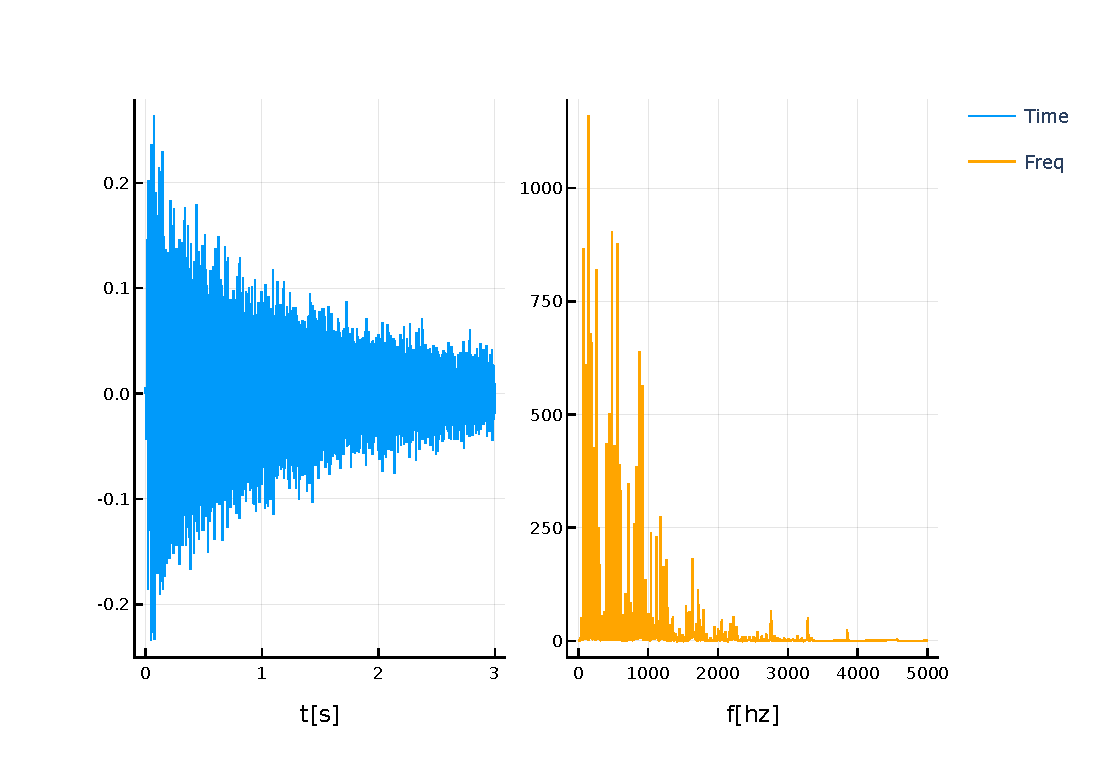
\includegraphics[width=1.0\linewidth]{assets/D1.pdf}
		\caption{D1}
		\label{fig:d1}
	\end{subfigure}%
	\begin{subfigure}{.5\textwidth}
		\centering
		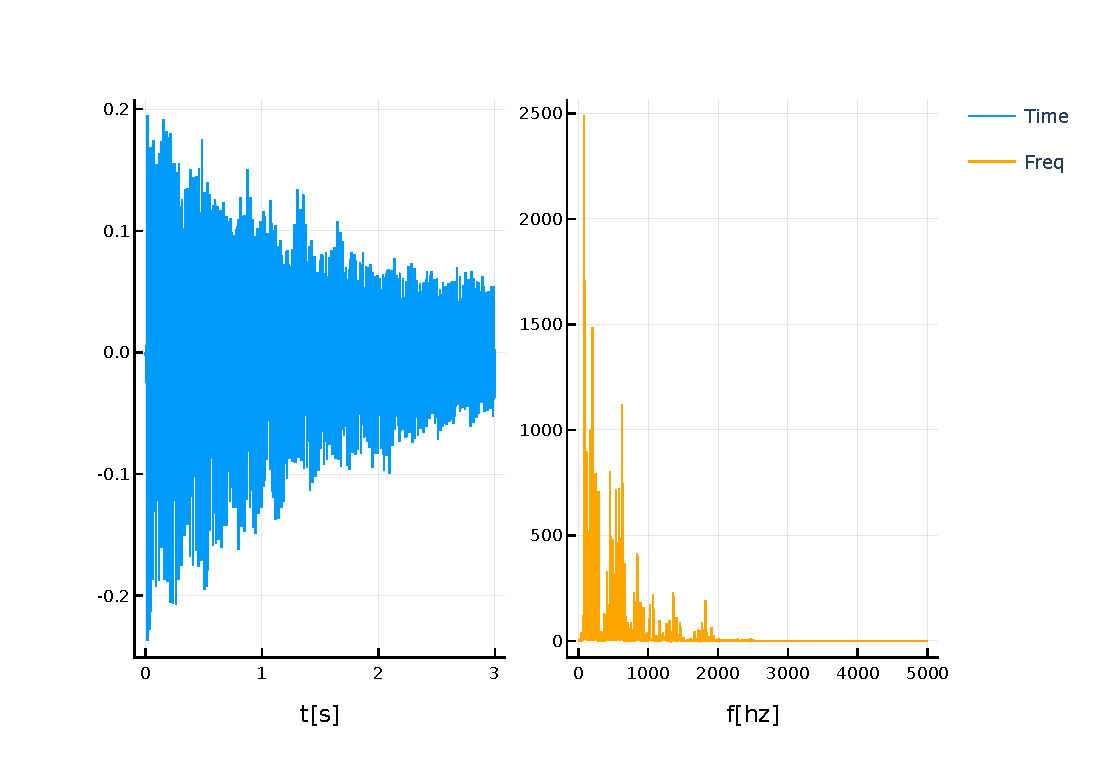
\includegraphics[width=1.0\linewidth]{assets/E1.pdf}
		\caption{E1}
		\label{fig:e1}
	\end{subfigure}
	\caption{}
\end{figure}

\begin{figure}[!ht]
	\centering
	\begin{subfigure}{.5\textwidth}
		\centering
		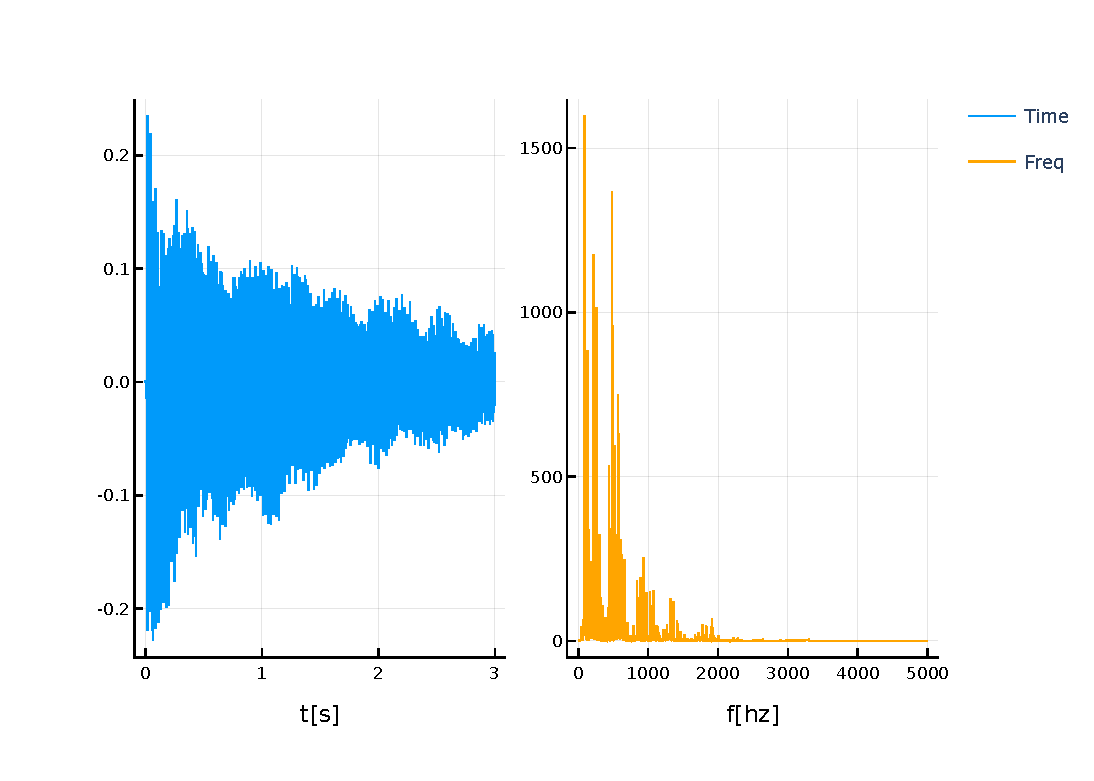
\includegraphics[width=1.0\linewidth]{assets/F1.pdf}
		\caption{F1}
		\label{fig:f1}
	\end{subfigure}%
	\begin{subfigure}{.5\textwidth}
		\centering
		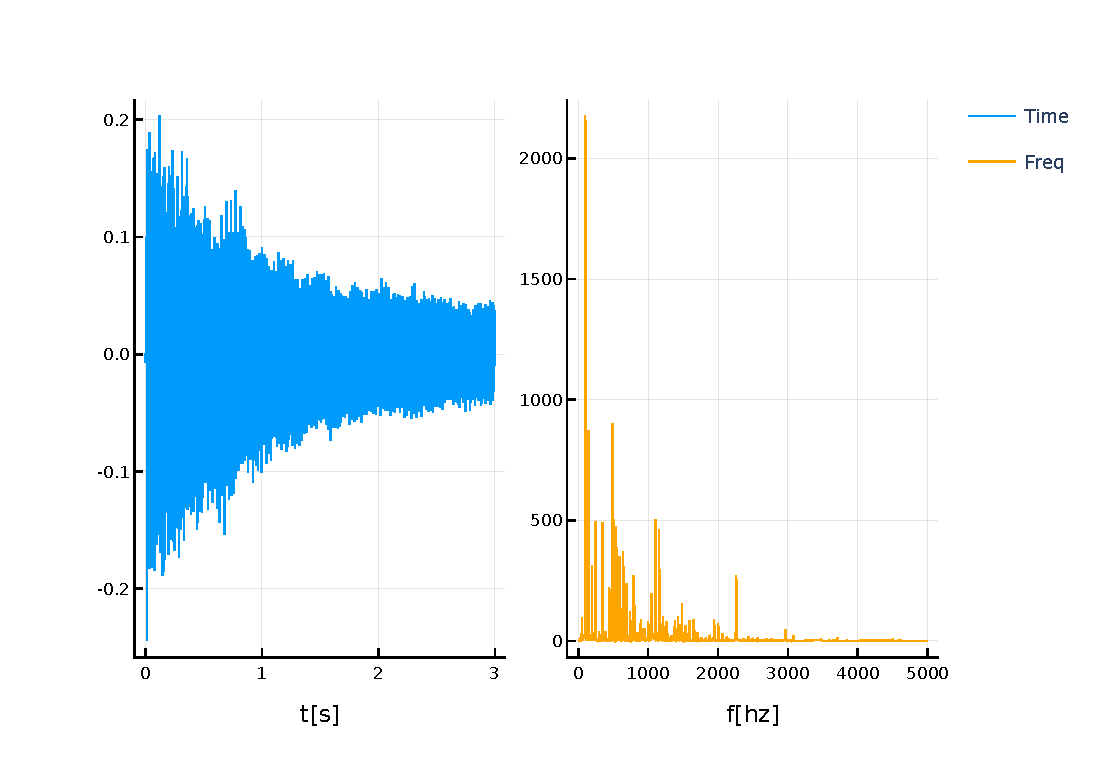
\includegraphics[width=1.0\linewidth]{assets/G1.pdf}
		\caption{G1}
		\label{fig:g1}
	\end{subfigure}
	\caption{}
\end{figure}

\bigskip
Como en esta aproximación aumentamos mucho el número de clases a clasificar (50 en total),
nos parece buena opción aumentar también las características utilizadas, pero desde un enfoque
diferente a la anterior aproximación. Lo que haremos será aumentar el número de intervalos
a dividir el dominio de la frecuencia; de 10 intervalos que teníamos anteriormente, a 30 intervalos.
De esta manera, esperamos que se puede clasificar mejor notas que tengan frecuencias muy cercanas,
además de repartir mejor el número de notas que coinciden en cada intervalo.

\newpage
En concreto, los intervalos de frecuencias que utilizaremos serán los siguientes:

\textit{(0.0, 63.845)},\textit{(63.845, 131.486)}, 
\textit{(131.486, 203.149)},\textit{(203.149, 279.074)}, 
\textit{(279.074, 359.513)},\textit{(359.513, 444.735)}, 
\textit{(444.735, 535.025)},\textit{(535.025, 630.684)}, 
\textit{(630.684, 732.032)}, \textit{(732.032, 839.405)},
\textit{(839.405, 953.163)}, \textit{(953.163, 1073.686)},
\textit{(1073.686, 1201.376)}, \textit{(1201.376, 1336.658)}, 
\textit{(1336.658, 1479.984)}, \textit{(1479.984, 1631.833)},
\textit{(1631.833, 1792.712)}, \textit{(1792.712, 1963.157)},
\textit{(1963.157, 2143.737)}, \textit{(2143.737, 2335.055)}, 
\textit{(2335.055, 2537.749)}, \textit{(2537.749, 2752.496)}, 
\textit{(2752.496, 2980.013)}, \textit{(2980.013, 3221.059)}, 
\textit{(3221.059, 3476.437)}, \textit{(3476.437, 3747.002)},
\textit{(3747.002, 4033.655)}, \textit{(4033.655, 4337.353)},
\textit{(4337.353, 4659.11)} y \textit{(4659.11, 5000.0)}

Para el preprocesado de los datos, utilizaremos, como se mencionó en aproximaciones anteriores,
una normalización de media cero.
Así, obtuvimos para cada característica, la media y la desviación típica. Se muestran dichos datos en las Tablas \ref{Tab:Features_3_1},
\ref{Tab:Features_3_2} \ref{Tab:Features_3_3} y \ref{Tab:Features_3_4}.

\begin{table}
	\caption{Parámetros de normalización (I)}
	\centering
		\begin{tabular}{||c c c||}
			\hline
			Característica & Media & Desviación Típica  \\ [0.5ex]
			\hline\hline
			E & $0.0054126005$ & $0.009019938$ \\
			\hline
			zero-crossing & $3397.5913$ & $4540.8813$ \\
			\hline
			m\textsubscript{1} & $2.5406487$ & $5.2477403$ \\
			\hline
			m\textsubscript{2} & $20.31295$ & $34.20369$ \\
			\hline
			m\textsubscript{3} & $18.736494$ & $33.777767$ \\
			\hline
			m\textsubscript{4} & $19.506176$ & $27.648252$ \\
			\hline
			m\textsubscript{5} & $17.283388$ & $26.778984$ \\
			\hline
			m\textsubscript{6} & $14.071337$ & $21.961533$ \\
			\hline
			m\textsubscript{7} & $15.653144$ & $21.659325$ \\
			\hline
			m\textsubscript{8} & $7.2894015$ & $11.942419$ \\
			\hline
			m\textsubscript{9} & $10.673911$ & $22.342806$ \\
			\hline
			m\textsubscript{10} & $8.886631$ & $17.860262$ \\
			\hline
			m\textsubscript{11} & $8.768464$ & $14.431124$ \\
			\hline
			m\textsubscript{12} & $9.399654$ & $13.1116905$ \\
			\hline
			m\textsubscript{13} & $7.141891$ & $16.054686$ \\
			\hline
			m\textsubscript{14} & $5.671832$ & $9.146762$ \\
			\hline
			m\textsubscript{15} & $4.4691596$ & $7.688136$ \\
			\hline
			m\textsubscript{16} & $4.622483$ & $7.50842$ \\
			\hline
			m\textsubscript{17} & $2.8246067$ & $5.453456$ \\
			\hline
			m\textsubscript{18} & $2.1192815$ & $3.5254076$ \\
			\hline
			m\textsubscript{19} & $3.2075806$ & $5.558346$ \\
			\hline
			m\textsubscript{20} & $1.3101652$ & $2.2760432$ \\
			\hline
			m\textsubscript{21} & $1.5997506$ & $4.51931$ \\
			\hline
			m\textsubscript{22} & $1.4330753$ & $3.7737772$ \\
			\hline
			m\textsubscript{23} & $0.9662523$ & $2.9858894$ \\
			\hline
			m\textsubscript{24} & $0.79353756$ & $1.8264828$ \\
			\hline
			m\textsubscript{25} & $0.48343834$ & $0.8716932$ \\
			\hline
			m\textsubscript{26} & $0.6009706$ & $1.4477166$ \\
			\hline
			m\textsubscript{27} & $0.3706837$ & $0.93128383$ \\
			\hline
			m\textsubscript{28} & $0.41856125$ & $1.3392309$ \\
			\hline
			m\textsubscript{29} & $0.38214317$ & $1.6580197$ \\
			\hline
			m\textsubscript{30} & $0.13477807$ & $0.25888646$ \\
			\hline
		\end{tabular}
	\label{Tab:Features_3_1}
\end{table}

\begin{table}
	\caption{Parámetros de normalización (II)}
	\centering
		\begin{tabular}{||c c c||}
			\hline
			Característica & Media & Desviación Típica  \\ [0.5ex]
			\hline\hline
			std\textsubscript{1} & $3.777772$ & $9.5573845$ \\
			\hline
			std\textsubscript{2} & $43.746407$ & $101.179634$ \\
			\hline
			std\textsubscript{3} & $44.765743$ & $106.52451$ \\
			\hline
			std\textsubscript{4} & $44.928486$ & $86.98192$ \\
			\hline
			std\textsubscript{5} & $36.79204$ & $74.466835$ \\
			\hline
			std\textsubscript{6} & $34.05622$ & $69.12505$ \\
			\hline
			std\textsubscript{7} & $35.642204$ & $58.005997$ \\
			\hline
			std\textsubscript{8} & $14.239829$ & $31.195595$ \\
			\hline
			std\textsubscript{9} & $20.148722$ & $46.739002$ \\
			\hline
			std\textsubscript{10} & $18.305641$ & $41.97697$ \\
			\hline
			std\textsubscript{11} & $15.096799$ & $33.64003$ \\
			\hline
			std\textsubscript{12} & $17.944155$ & $31.481377$ \\
			\hline
			std\textsubscript{13} & $14.973824$ & $42.54836$ \\
			\hline
			std\textsubscript{14} & $10.101966$ & $21.576153$ \\
			\hline
			std\textsubscript{15} & $7.4685116$ & $17.61445$ \\
			\hline
			std\textsubscript{16} & $7.9542217$ & $17.202675$ \\
			\hline
			std\textsubscript{17} & $5.18349$ & $11.849964$ \\
			\hline
			std\textsubscript{18} & $2.358577$ & $5.2823844$ \\
			\hline
			std\textsubscript{19} & $6.350091$ & $12.173027$ \\
			\hline
			std\textsubscript{20} & $1.757622$ & $4.281193$ \\
			\hline
			std\textsubscript{21} & $2.7778556$ & $8.633124$ \\
			\hline
			std\textsubscript{22} & $2.4016538$ & $6.636576$ \\
			\hline
			std\textsubscript{23} & $1.6487495$ & $5.640244$ \\
			\hline
			std\textsubscript{24} & $1.3393545$ & $3.0001454$ \\
			\hline
			std\textsubscript{25} & $0.606615$ & $1.4506007$ \\
			\hline
			std\textsubscript{26} & $0.9203455$ & $2.2596686$ \\
			\hline
			std\textsubscript{27} & $0.4674074$ & $1.0911392$ \\
			\hline
			std\textsubscript{28} & $0.64302534$ & $2.1712365$ \\
			\hline
			std\textsubscript{29} & $0.45122066$ & $1.628174$ \\
			\hline
			std\textsubscript{30} & $0.19327588$ & $0.4538704$ \\
			\hline
		\end{tabular}
	\label{Tab:Features_3_2}
\end{table}

\begin{table}
	\caption{Parámetros de normalización (III)}
	\centering
		\begin{tabular}{||c c c||}
			\hline
			Característica & Media & Desviación Típica  \\ [0.5ex]
			\hline\hline
			max\textsubscript{1} & $33.78178$ & $108.59057$ \\
			\hline
			max\textsubscript{2} & $448.6926$ & $1190.1057$ \\
			\hline
			max\textsubscript{3} & $473.44827$ & $1207.2843$ \\
			\hline
			max\textsubscript{4} & $464.8955$ & $994.3883$ \\
			\hline
			max\textsubscript{5} & $362.47415$ & $770.89215$ \\
			\hline
			max\textsubscript{6} & $343.7377$ & $698.5618$ \\
			\hline
			max\textsubscript{7} & $339.793$ & $571.1343$ \\
			\hline
			max\textsubscript{8} & $146.53598$ & $331.86856$ \\
			\hline
			max\textsubscript{9} & $187.07274$ & $410.4047$ \\
			\hline
			max\textsubscript{10} & $172.76352$ & $362.9538$ \\
			\hline
			max\textsubscript{11} & $142.42677$ & $321.43628$ \\
			\hline
			max\textsubscript{12} & $170.99661$ & $295.21555$ \\
			\hline
			max\textsubscript{13} & $140.03787$ & $364.36176$ \\
			\hline
			max\textsubscript{14} & $98.230865$ & $208.93227$ \\
			\hline
			max\textsubscript{15} & $68.81298$ & $154.13226$ \\
			\hline
			max\textsubscript{16} & $74.12923$ & $160.24773$ \\
			\hline
			max\textsubscript{17} & $51.78036$ & $117.74015$ \\
			\hline
			max\textsubscript{18} & $20.73961$ & $55.032047$ \\
			\hline
			max\textsubscript{19} & $55.946613$ & $99.87239$ \\
			\hline
			max\textsubscript{20} & $16.036867$ & $44.92402$ \\
			\hline
			max\textsubscript{21} & $23.404562$ & $60.15183$ \\
			\hline
			max\textsubscript{22} & $19.944548$ & $46.585274$ \\
			\hline
			max\textsubscript{23} & $14.242097$ & $44.026596$ \\
			\hline
			max\textsubscript{24} & $11.504292$ & $23.90699$ \\
			\hline
			max\textsubscript{25} & $5.2844114$ & $13.773306$ \\
			\hline
			max\textsubscript{26} & $7.49625$ & $17.74915$ \\
			\hline
			max\textsubscript{27} & $3.6148624$ & $8.03344$ \\
			\hline
			max\textsubscript{28} & $4.8835807$ & $14.053778$ \\
			\hline
			max\textsubscript{29} & $3.2500324$ & $9.766679$ \\
			\hline
			max\textsubscript{30} & $1.6198401$ & $3.8292391$ \\
			\hline
		\end{tabular}
	\label{Tab:Features_3_3}
\end{table}

\begin{table}
	\caption{Parámetros de normalización (IV)}
	\centering
		\begin{tabular}{||c c c||}
			\hline
			Característica & Media & Desviación Típica  \\ [0.5ex]
			\hline\hline
			max-freq\textsubscript{1} & $35.377235$ & $14.779791$ \\
			\hline
			max-freq\textsubscript{2} & $109.41023$ & $14.310052$ \\
			\hline
			max-freq\textsubscript{3} & $157.08893$ & $22.204115$ \\
			\hline
			max-freq\textsubscript{4} & $237.34592$ & $25.370153$ \\
			\hline
			max-freq\textsubscript{5} & $310.14645$ & $24.312443$ \\
			\hline
			max-freq\textsubscript{6} & $403.7519$ & $27.410894$ \\
			\hline
			max-freq\textsubscript{7} & $489.3408$ & $23.016937$ \\
			\hline
			max-freq\textsubscript{8} & $584.6093$ & $31.939516$ \\
			\hline
			max-freq\textsubscript{9} & $672.22675$ & $27.801172$ \\
			\hline
			max-freq\textsubscript{10} & $781.4551$ & $30.98548$ \\
			\hline
			max-freq\textsubscript{11} & $904.9106$ & $33.565907$ \\
			\hline
			max-freq\textsubscript{12} & $1004.27$ & $35.98437$ \\
			\hline
			max-freq\textsubscript{13} & $1136.5785$ & $49.034184$ \\
			\hline
			max-freq\textsubscript{14} & $1269.4824$ & $45.24625$ \\
			\hline
			max-freq\textsubscript{15} & $1409.3927$ & $50.92556$ \\
			\hline
			max-freq\textsubscript{16} & $1535.1046$ & $41.005337$ \\
			\hline
			max-freq\textsubscript{17} & $1704.3861$ & $49.30979$ \\
			\hline
			max-freq\textsubscript{18} & $1873.1862$ & $58.287815$ \\
			\hline
			max-freq\textsubscript{19} & $2052.2415$ & $60.40939$ \\
			\hline
			max-freq\textsubscript{20} & $2217.6611$ & $66.80756$ \\
			\hline
			max-freq\textsubscript{21} & $2417.3076$ & $57.010002$ \\
			\hline
			max-freq\textsubscript{22} & $2638.4033$ & $58.779163$ \\
			\hline
			max-freq\textsubscript{23} & $2857.4375$ & $74.33377$ \\
			\hline
			max-freq\textsubscript{24} & $3086.9392$ & $80.97323$ \\
			\hline
			max-freq\textsubscript{25} & $3342.3274$ & $80.32275$ \\
			\hline
			max-freq\textsubscript{26} & $3589.7864$ & $78.69773$ \\
			\hline
			max-freq\textsubscript{27} & $3879.9844$ & $98.408936$ \\
			\hline
			max-freq\textsubscript{28} & $4168.601$ & $103.71468$ \\
			\hline
			max-freq\textsubscript{29} & $4459.1206$ & $91.55003$ \\
			\hline
			max-freq\textsubscript{30} & $4837.6816$ & $100.40303$ \\
			\hline
		\end{tabular}
	\label{Tab:Features_3_4}
\end{table}

\newpage
\hphantom{skip}

Donde:
\begin{itemize}
	\item \textit{E} indica la \textbf{energía de la señal}.
	\item \textit{m\textsubscript{i}} indica la \textbf{media de la intensidad} en el intervalo \textit{i} en frecuencia.
	\item \textit{std\textsubscript{i}} indica la \textbf{desviación típica de la intensidad} en el intervalo \textit{i} en frecuencia.
	\item \textit{max\textsubscript{i}} indica el \textbf{máximo de la intensidad} en el intervalo \textit{i} en frecuencia.
	\item \textit{max-freq\textsubscript{i}} indica la \textbf{frecuencia donde se alcanza el máximo de intensidad} en el intervalo \textit{i} en frecuencia.
\end{itemize}
Para estos experimentos se ha repetido 20 veces el entrenamiento de la RNA en cada \textit{fold}, devolviendo el resultado promedio de esas 20 ejecuciones.

\bigskip
Para poder evaluar el modelo con mejor rendimiento, como ya se ha dicho anteriormente, utilizaremos como medida el promedio
del \textbf{F1-Score} en los \textit{folds}. Si hay empate en dicha media, se elegirá el modelo con menor
desviación típica de la métrica.

\subsubsection{Resultados}
Para permitir la reproducibilidad de los experimentos, se utilizó \textit{100} como semilla de generación de números
aleatorios.

\paragraph{RNA}

Para el entrenamiento de las RNA, se han utilizado los siguientes parámetros en común:
\begin{itemize}
	\item Ratio de aprendizaje: $0.01$
	\item Ratio de patrones para el conjunto de validación: $0.2$.
	\item Máximo número de ciclos (\textit{epochs}) de entrenamiento: $1500$.
	\item Máximo número de ciclos (\textit{epochs}) de entrenamiento sin mejorar el error de validación: $5$.
	\item Algoritmo de optimización: ADAM.
	\item Función de \textit{loss}: \textit{Cross Entropy}.
\end{itemize}
El hiperparámetro que hemos variado ha sido la arquitectura de neuronas a utilizar. Utilizamos 8 arquitecturas distintas,
donde la arquitectura [$i$] denota una RNA con una única capa oculta con $i$ neuronas y la arquitectura [$i$, $j$] 
denota una neurona con dos capas ocultas; con $i$ neuronas en la primera capa oculta y $j$ neuronas en la segunda capa oculta.

Se muestran los resultados de la experimentación en la Tabla \ref{Tab:ANN_3}.

\begin{table}[!ht]
	\caption{Resultados RNA}
	\centering
		 \begin{tabular}{||c c c||}
			 \hline
			 Arquitectura & F1-Score & Precisión  \\ [0.5ex]
			 \hline\hline
		[16] & $0.95148 \pm 0.00551$ & $0.96105 \pm 0.00471$ \\
		\hline 
		[32] & $0.98759 \pm 0.00345$ & $0.9897 \pm 0.00221$ \\
		\hline 
		[64] & $0.99345 \pm 0.00309$ & $0.99428 \pm 0.00162$ \\
		\hline 
		[128] & $0.99293 \pm 0.00258$ & $0.99424 \pm 0.00123$ \\
		\hline 
		[256] & $0.99269 \pm 0.00345$ & $0.9936 \pm 0.00299$ \\
		\hline 
		[512] & $0.98348 \pm 0.0061$ & $0.98603 \pm 0.00423$ \\
		\hline 
		[64, 64] & $0.98322 \pm 0.00373$ & $0.98554 \pm 0.00292$ \\
		\hline 
		[64, 128] & $0.9818 \pm 0.00226$ & $0.98428 \pm 0.00227$ \\
		\hline 
		 \end{tabular}
	\label{Tab:ANN_3}
	\end{table}

\paragraph{SVM}

Para las máquinas de soporte vectorial hemos utilizado 8 configuraciones distintas de los hiperparámetros de \textit{kernel},
grado del \textit{kernel} (sólo se utiliza en \textit{kernel} polinomial), \textit{gamma} y \textit{C}.

Se muestran los resultados de la experimentación en la Tabla \ref{Tab:SVM_3}.

\begin{table}[!ht]
	\caption{Resultados SVM}
	\centering
		 \begin{tabular}{||c c c||}
			 \hline
			 (kernel, grado, gamma, C) & F1-Score & Precisión  \\ [0.5ex]
			 \hline\hline
			 (poly, $3$, $1$, $1$) & $0.99264 \pm 0.0053$ & $0.99382 \pm 0.00422$ \\
			\hline
			(rbf, $3$, $1$, $1$) & $0.10019 \pm 0.01854$ & $0.11513 \pm 0.0161$ \\
			\hline
			(sigmoid, $3$, $1$, $1$) & $0.13051 \pm 0.02229$ & $0.20283 \pm 0.02546$ \\
			\hline
			(poly, $3$, $10$, $0.1$) & $0.99113 \pm 0.00724$ & $0.99314 \pm 0.00464$ \\
			\hline
			(rbf, $3$, $10$, $0.1$) & $0.00179 \pm 7.0e-5$ & $0.04673 \pm 0.00189$ \\
			\hline
			(sigmoid, $3$, $10$, $0.1$) & $0.10752 \pm 0.01502$ & $0.18363 \pm 0.01528$ \\
			\hline
			(rbf, $3$, $0.01$, $100$) & $0.99504 \pm 0.00411$ & $0.99563 \pm 0.00257$ \\
			\hline
			(poly, $3$, $100$, $0.001$) & $0.99257 \pm 0.00408$ & $0.99379 \pm 0.00278$ \\
			\hline
		 \end{tabular}
	\label{Tab:SVM_3}
	\end{table}

\paragraph{Árboles de decisión}
Para los árboles de decisión hemos utilizado 6 configuraciones distintas del hiperparámetro de profundidad máxima.

Se muestran los resultados de la experimentación en la Tabla \ref{Tab:DecisionTree_3}.

\begin{table}[!ht]
	\caption{Resultados Árbol de decisión}
	\centering
		 \begin{tabular}{||c c c||}
			 \hline
			 Altura máxima & F1-Score & Precisión  \\ [0.5ex]
			 \hline\hline
			 $4$ & $0.09189 \pm 0.01043$ & $0.17819 \pm 0.0157$ \\
			\hline
			$8$ & $0.3111 \pm 0.01697$ & $0.42453 \pm 0.01404$ \\
			\hline
			$16$ & $0.71777 \pm 0.04105$ & $0.79892 \pm 0.03264$ \\
			\hline
			$32$ & $0.94074 \pm 0.01447$ & $0.94584 \pm 0.01159$ \\
			\hline
			$64$ & $0.94887 \pm 0.01332$ & $0.95193 \pm 0.01202$ \\
			\hline
			$128$ & $0.95088 \pm 0.00891$ & $0.9555 \pm 0.00573$ \\
			\hline
			$256$ & $0.95003 \pm 0.00775$ & $0.95269 \pm 0.0076$ \\
			\hline
		 \end{tabular}
	\label{Tab:DecisionTree_3}
	\end{table}

\paragraph{kNN}
Para el modelo kNN hemos utilizado 6 configuraciones distintas del hiperparámetro de k (número de vecinos más cercanos).

Se muestran los resultados de la experimentación en la tabla \ref{Tab:kNN_3}.

\begin{table}[!ht]
	\caption{Resultados kNN}
	\centering
		 \begin{tabular}{||c c c||}
			 \hline
			 K & F1-Score & Precisión  \\ [0.5ex]
			 \hline\hline
			 $2$ & $0.98683 \pm 0.00434$ & $0.98845 \pm 0.00303$ \\
			\hline
			$3$ & $0.98153 \pm 0.00991$ & $0.98636 \pm 0.00479$ \\
			\hline
			$5$ & $0.98086 \pm 0.00835$ & $0.98617 \pm 0.00599$ \\
			\hline
			$8$ & $0.97161 \pm 0.01603$ & $0.98024 \pm 0.01049$ \\
			\hline
			$13$ & $0.96203 \pm 0.01287$ & $0.97342 \pm 0.00864$ \\
			\hline
			$21$ & $0.95836 \pm 0.00902$ & $0.96928 \pm 0.00517$ \\
			\hline
		 \end{tabular}
	\label{Tab:kNN_3}
\end{table}

\newpage
\subsubsection{Discusión}
Los resultados de esta iteración son muy buenos, ya que hemos aumentado en gran medida el número de notas
a clasificar y hemos conseguido varios modelos con más de un 99\% de F1-Score y precisión. 

\bigskip
En concreto, el modelo que mejor funciona es un SVM con un \textit{kernel} de base radial y con valores de \textit{gamma} y
\textit{C} de $0.01$ y $100$, respectivamente. Este modelo alcanzó un F1-Score de 
$0.99594 \pm 0.00411$ y una precisión de $0.99563 \pm 0.00257$, unos valores muy altos y que indican
que el sistema funciona muy bien. 

\bigskip
Caben destacar también modelos que alcanzan un rendimiento parecido,
como puede ser un SVM con un \textit{kernel} polinomial de grado $3$, con ambos valores de \textit{gamma} y \textit{C} de $1$,
además de una RNA con una única capa oculta con $32$ neuronas.

\bigskip
En contra, el modelo que peor rendimiento presenta es un SVM con un \textit{kernel} de base radial,
con valores de \textit{gamma} y \textit{C} de $10$ y $0.1$, respectivamente. Cabe destacar que este modelo
es similar al modelo que presenta el mejor rendimiento, siendo lo único que cambia los parámetros de
\textit{gamma} y \textit{C}. Es notable ver que un ligero cambio en estos dos parámetros puede 
producir que un sistema pase de ser muy malo, a ser muchísimo mejor.

\bigskip
Como hemos podido ver, los resultados son muy buenos en general, pero algunos de estos sistemas tienen un problema (principalmente las RNAs),
y es que el tiempo de entrenamiento es mucho mayor que en aproximaciones anteriores. Creemos que esto se puede deber tanto por
aumentar el número de instancias a utilizar por el sistema (anteriormente $1090$, y en esta aproximación $3194$),
como por el número de características que se utilizan ($122$).
Así, y ante resultados tan satisfactorios, creemos que en futuras aproximaciones deberíamos intentar reducir el número de características, 
siempre tratando de no perder el rendimiento
de clasificación del sistema, permitiéndonos producir modelos que sean más rápidos de entrenar, a la vez que más rápidos
para realizar predicciones ante nuevos patrones.

\bigskip
En la matriz de confusión de la Tabla \ref{tab:confusion_matrix_3} hemos omitido por razones de tamaño las filas y las columnas donde 
el sistema no se confunde, a excepción de las 5 primeras y las 8 ultimas para definir el rango de notas de esta aproximación y su 
patrón diagonal de aciertos. Al igual que anteriores aproximaciones podemos destacar que los fallos son entre notas con frecuencias muy
parecidas como pueden ser \textit{G1}(\textit{48,99 Hz}) y \textit{A1}(\textit{55 Hz}) o \textit{G1}(\textit{48,99 Hz}) y \textit{E2}(\textit{82,40 Hz}).

\begin{table}[!ht]
	\centering
	\resizebox{\textwidth}{!}{
		\begin{tabular}{cccccccccccccccccccccccccccccccccccccc}
			&                          & \multicolumn{36}{c}{Predicc.}                                                                                                                                                                                                                                                                                                                                                                                                                                                                                                                                                                                                                                                                                                                                                                                                                                                                                                                                                                                                                 \\ \cline{3-38} 
			& \multicolumn{1}{c|}{}    & \multicolumn{1}{c|}{C1} & \multicolumn{1}{c|}{C2} & \multicolumn{1}{c|}{C3} & \multicolumn{1}{c|}{C4} & \multicolumn{1}{c|}{C5} & \multicolumn{1}{c|}{C6} & \multicolumn{1}{c|}{C7} & \multicolumn{1}{c|}{C8} & \multicolumn{1}{c|}{A1} & \multicolumn{1}{c|}{A2} & \multicolumn{1}{c|}{...}                  & \multicolumn{1}{c|}{B4} & \multicolumn{1}{c|}{B5} & \multicolumn{1}{c|}{B6} & \multicolumn{1}{c|}{B7} & \multicolumn{1}{c|}{D1} & \multicolumn{1}{c|}{...}                  & \multicolumn{1}{c|}{E1} & \multicolumn{1}{c|}{E2} & \multicolumn{1}{c|}{E3} & \multicolumn{1}{c|}{...}                  & \multicolumn{1}{c|}{E6} & \multicolumn{1}{c|}{E7} & \multicolumn{1}{c|}{F1} & \multicolumn{1}{c|}{F2} & \multicolumn{1}{c|}{F3} & \multicolumn{1}{c|}{...}                  & \multicolumn{1}{c|}{F6} & \multicolumn{1}{c|}{F7} & \multicolumn{1}{c|}{G1} & \multicolumn{1}{c|}{G2} & \multicolumn{1}{c|}{G3} & \multicolumn{1}{c|}{G4} & \multicolumn{1}{c|}{G5} & \multicolumn{1}{c|}{G6} & \multicolumn{1}{c|}{G7} \\ \cline{2-38} 
\multicolumn{1}{c|}{\multirow{22}{*}{Real}} & \multicolumn{1}{c|}{C1}  & \multicolumn{1}{c|}{7}  & \multicolumn{1}{c|}{0}  & \multicolumn{1}{c|}{0}  & \multicolumn{1}{c|}{0}  & \multicolumn{1}{c|}{0}  & \multicolumn{1}{c|}{0}  & \multicolumn{1}{c|}{0}  & \multicolumn{1}{c|}{0}  & \multicolumn{1}{c|}{0}  & \multicolumn{1}{c|}{0}  & \multicolumn{1}{c|}{\multirow{5}{*}{,,,}} & \multicolumn{1}{c|}{0}  & \multicolumn{1}{c|}{0}  & \multicolumn{1}{c|}{0}  & \multicolumn{1}{c|}{0}  & \multicolumn{1}{c|}{0}  & \multicolumn{1}{c|}{\multirow{5}{*}{,,,}} & \multicolumn{1}{c|}{0}  & \multicolumn{1}{c|}{0}  & \multicolumn{1}{c|}{0}  & \multicolumn{1}{c|}{\multirow{5}{*}{,,,}} & \multicolumn{1}{c|}{0}  & \multicolumn{1}{c|}{0}  & \multicolumn{1}{c|}{0}  & \multicolumn{1}{c|}{0}  & \multicolumn{1}{c|}{0}  & \multicolumn{1}{c|}{\multirow{5}{*}{,,,}} & \multicolumn{1}{c|}{0}  & \multicolumn{1}{c|}{0}  & \multicolumn{1}{c|}{0}  & \multicolumn{1}{c|}{0}  & \multicolumn{1}{c|}{0}  & \multicolumn{1}{c|}{0}  & \multicolumn{1}{c|}{0}  & \multicolumn{1}{c|}{0}  & \multicolumn{1}{c|}{0}  \\ \cline{2-12} \cline{14-18} \cline{20-22} \cline{24-28} \cline{30-38} 
\multicolumn{1}{c|}{}                       & \multicolumn{1}{c|}{C2}  & \multicolumn{1}{c|}{0}  & \multicolumn{1}{c|}{7}  & \multicolumn{1}{c|}{0}  & \multicolumn{1}{c|}{0}  & \multicolumn{1}{c|}{0}  & \multicolumn{1}{c|}{0}  & \multicolumn{1}{c|}{0}  & \multicolumn{1}{c|}{0}  & \multicolumn{1}{c|}{0}  & \multicolumn{1}{c|}{0}  & \multicolumn{1}{c|}{}                     & \multicolumn{1}{c|}{0}  & \multicolumn{1}{c|}{0}  & \multicolumn{1}{c|}{0}  & \multicolumn{1}{c|}{0}  & \multicolumn{1}{c|}{0}  & \multicolumn{1}{c|}{}                     & \multicolumn{1}{c|}{0}  & \multicolumn{1}{c|}{0}  & \multicolumn{1}{c|}{0}  & \multicolumn{1}{c|}{}                     & \multicolumn{1}{c|}{0}  & \multicolumn{1}{c|}{0}  & \multicolumn{1}{c|}{0}  & \multicolumn{1}{c|}{0}  & \multicolumn{1}{c|}{0}  & \multicolumn{1}{c|}{}                     & \multicolumn{1}{c|}{0}  & \multicolumn{1}{c|}{0}  & \multicolumn{1}{c|}{0}  & \multicolumn{1}{c|}{0}  & \multicolumn{1}{c|}{0}  & \multicolumn{1}{c|}{0}  & \multicolumn{1}{c|}{0}  & \multicolumn{1}{c|}{0}  & \multicolumn{1}{c|}{0}  \\ \cline{2-12} \cline{14-18} \cline{20-22} \cline{24-28} \cline{30-38} 
\multicolumn{1}{c|}{}                       & \multicolumn{1}{c|}{C3}  & \multicolumn{1}{c|}{0}  & \multicolumn{1}{c|}{0}  & \multicolumn{1}{c|}{11} & \multicolumn{1}{c|}{0}  & \multicolumn{1}{c|}{0}  & \multicolumn{1}{c|}{0}  & \multicolumn{1}{c|}{0}  & \multicolumn{1}{c|}{0}  & \multicolumn{1}{c|}{0}  & \multicolumn{1}{c|}{0}  & \multicolumn{1}{c|}{}                     & \multicolumn{1}{c|}{0}  & \multicolumn{1}{c|}{0}  & \multicolumn{1}{c|}{0}  & \multicolumn{1}{c|}{0}  & \multicolumn{1}{c|}{0}  & \multicolumn{1}{c|}{}                     & \multicolumn{1}{c|}{0}  & \multicolumn{1}{c|}{0}  & \multicolumn{1}{c|}{0}  & \multicolumn{1}{c|}{}                     & \multicolumn{1}{c|}{0}  & \multicolumn{1}{c|}{0}  & \multicolumn{1}{c|}{0}  & \multicolumn{1}{c|}{0}  & \multicolumn{1}{c|}{0}  & \multicolumn{1}{c|}{}                     & \multicolumn{1}{c|}{0}  & \multicolumn{1}{c|}{0}  & \multicolumn{1}{c|}{0}  & \multicolumn{1}{c|}{0}  & \multicolumn{1}{c|}{0}  & \multicolumn{1}{c|}{0}  & \multicolumn{1}{c|}{0}  & \multicolumn{1}{c|}{0}  & \multicolumn{1}{c|}{0}  \\ \cline{2-12} \cline{14-18} \cline{20-22} \cline{24-28} \cline{30-38} 
\multicolumn{1}{c|}{}                       & \multicolumn{1}{c|}{C4}  & \multicolumn{1}{c|}{0}  & \multicolumn{1}{c|}{0}  & \multicolumn{1}{c|}{0}  & \multicolumn{1}{c|}{15} & \multicolumn{1}{c|}{0}  & \multicolumn{1}{c|}{0}  & \multicolumn{1}{c|}{0}  & \multicolumn{1}{c|}{0}  & \multicolumn{1}{c|}{0}  & \multicolumn{1}{c|}{0}  & \multicolumn{1}{c|}{}                     & \multicolumn{1}{c|}{0}  & \multicolumn{1}{c|}{0}  & \multicolumn{1}{c|}{0}  & \multicolumn{1}{c|}{0}  & \multicolumn{1}{c|}{0}  & \multicolumn{1}{c|}{}                     & \multicolumn{1}{c|}{0}  & \multicolumn{1}{c|}{0}  & \multicolumn{1}{c|}{0}  & \multicolumn{1}{c|}{}                     & \multicolumn{1}{c|}{0}  & \multicolumn{1}{c|}{0}  & \multicolumn{1}{c|}{0}  & \multicolumn{1}{c|}{0}  & \multicolumn{1}{c|}{0}  & \multicolumn{1}{c|}{}                     & \multicolumn{1}{c|}{0}  & \multicolumn{1}{c|}{0}  & \multicolumn{1}{c|}{0}  & \multicolumn{1}{c|}{0}  & \multicolumn{1}{c|}{0}  & \multicolumn{1}{c|}{0}  & \multicolumn{1}{c|}{0}  & \multicolumn{1}{c|}{0}  & \multicolumn{1}{c|}{0}  \\ \cline{2-12} \cline{14-18} \cline{20-22} \cline{24-28} \cline{30-38} 
\multicolumn{1}{c|}{}                       & \multicolumn{1}{c|}{C5}  & \multicolumn{1}{c|}{0}  & \multicolumn{1}{c|}{0}  & \multicolumn{1}{c|}{0}  & \multicolumn{1}{c|}{0}  & \multicolumn{1}{c|}{32} & \multicolumn{1}{c|}{0}  & \multicolumn{1}{c|}{0}  & \multicolumn{1}{c|}{0}  & \multicolumn{1}{c|}{0}  & \multicolumn{1}{c|}{0}  & \multicolumn{1}{c|}{}                     & \multicolumn{1}{c|}{0}  & \multicolumn{1}{c|}{0}  & \multicolumn{1}{c|}{0}  & \multicolumn{1}{c|}{0}  & \multicolumn{1}{c|}{0}  & \multicolumn{1}{c|}{}                     & \multicolumn{1}{c|}{0}  & \multicolumn{1}{c|}{0}  & \multicolumn{1}{c|}{0}  & \multicolumn{1}{c|}{}                     & \multicolumn{1}{c|}{0}  & \multicolumn{1}{c|}{0}  & \multicolumn{1}{c|}{0}  & \multicolumn{1}{c|}{0}  & \multicolumn{1}{c|}{0}  & \multicolumn{1}{c|}{}                     & \multicolumn{1}{c|}{0}  & \multicolumn{1}{c|}{0}  & \multicolumn{1}{c|}{0}  & \multicolumn{1}{c|}{0}  & \multicolumn{1}{c|}{0}  & \multicolumn{1}{c|}{0}  & \multicolumn{1}{c|}{0}  & \multicolumn{1}{c|}{0}  & \multicolumn{1}{c|}{0}  \\ \cline{2-12} \cline{14-18} \cline{20-22} \cline{24-28} \cline{30-38} 
\multicolumn{1}{c|}{}                       & \multicolumn{1}{c|}{...} & \multicolumn{36}{c|}{...}                                                                                                                                                                                                                                                                                                                                                                                                                                                                                                                                                                                                                                                                                                                                                                                                                                                                                                                                                                                                                     \\ \cline{2-12} \cline{14-18} \cline{20-22} \cline{24-28} \cline{30-38} 
\multicolumn{1}{c|}{}                       & \multicolumn{1}{c|}{B5}  & \multicolumn{1}{c|}{0}  & \multicolumn{1}{c|}{0}  & \multicolumn{1}{c|}{0}  & \multicolumn{1}{c|}{0}  & \multicolumn{1}{c|}{0}  & \multicolumn{1}{c|}{0}  & \multicolumn{1}{c|}{0}  & \multicolumn{1}{c|}{0}  & \multicolumn{1}{c|}{0}  & \multicolumn{1}{c|}{0}  & \multicolumn{1}{c|}{\multirow{3}{*}{...}} & \multicolumn{1}{c|}{0}  & \multicolumn{1}{c|}{14} & \multicolumn{1}{c|}{0}  & \multicolumn{1}{c|}{0}  & \multicolumn{1}{c|}{0}  & \multicolumn{1}{c|}{\multirow{3}{*}{...}} & \multicolumn{1}{c|}{0}  & \multicolumn{1}{c|}{0}  & \multicolumn{1}{c|}{0}  & \multicolumn{1}{c|}{\multirow{3}{*}{...}} & \multicolumn{1}{c|}{0}  & \multicolumn{1}{c|}{0}  & \multicolumn{1}{c|}{0}  & \multicolumn{1}{c|}{0}  & \multicolumn{1}{c|}{0}  & \multicolumn{1}{c|}{\multirow{3}{*}{...}} & \multicolumn{1}{c|}{0}  & \multicolumn{1}{c|}{0}  & \multicolumn{1}{c|}{0}  & \multicolumn{1}{c|}{0}  & \multicolumn{1}{c|}{0}  & \multicolumn{1}{c|}{0}  & \multicolumn{1}{c|}{0}  & \multicolumn{1}{c|}{0}  & \multicolumn{1}{c|}{0}  \\ \cline{2-12} \cline{14-18} \cline{20-22} \cline{24-28} \cline{30-38} 
\multicolumn{1}{c|}{}                       & \multicolumn{1}{c|}{B6}  & \multicolumn{1}{c|}{0}  & \multicolumn{1}{c|}{0}  & \multicolumn{1}{c|}{0}  & \multicolumn{1}{c|}{0}  & \multicolumn{1}{c|}{0}  & \multicolumn{1}{c|}{0}  & \multicolumn{1}{c|}{0}  & \multicolumn{1}{c|}{1}  & \multicolumn{1}{c|}{0}  & \multicolumn{1}{c|}{0}  & \multicolumn{1}{c|}{}                     & \multicolumn{1}{c|}{0}  & \multicolumn{1}{c|}{0}  & \multicolumn{1}{c|}{18} & \multicolumn{1}{c|}{0}  & \multicolumn{1}{c|}{0}  & \multicolumn{1}{c|}{}                     & \multicolumn{1}{c|}{0}  & \multicolumn{1}{c|}{0}  & \multicolumn{1}{c|}{0}  & \multicolumn{1}{c|}{}                     & \multicolumn{1}{c|}{0}  & \multicolumn{1}{c|}{0}  & \multicolumn{1}{c|}{0}  & \multicolumn{1}{c|}{0}  & \multicolumn{1}{c|}{0}  & \multicolumn{1}{c|}{}                     & \multicolumn{1}{c|}{0}  & \multicolumn{1}{c|}{0}  & \multicolumn{1}{c|}{0}  & \multicolumn{1}{c|}{0}  & \multicolumn{1}{c|}{0}  & \multicolumn{1}{c|}{0}  & \multicolumn{1}{c|}{0}  & \multicolumn{1}{c|}{0}  & \multicolumn{1}{c|}{0}  \\ \cline{2-12} \cline{14-18} \cline{20-22} \cline{24-28} \cline{30-38} 
\multicolumn{1}{c|}{}                       & \multicolumn{1}{c|}{B7}  & \multicolumn{1}{c|}{0}  & \multicolumn{1}{c|}{0}  & \multicolumn{1}{c|}{0}  & \multicolumn{1}{c|}{0}  & \multicolumn{1}{c|}{0}  & \multicolumn{1}{c|}{0}  & \multicolumn{1}{c|}{0}  & \multicolumn{1}{c|}{0}  & \multicolumn{1}{c|}{0}  & \multicolumn{1}{c|}{0}  & \multicolumn{1}{c|}{}                     & \multicolumn{1}{c|}{0}  & \multicolumn{1}{c|}{0}  & \multicolumn{1}{c|}{0}  & \multicolumn{1}{c|}{14} & \multicolumn{1}{c|}{0}  & \multicolumn{1}{c|}{}                     & \multicolumn{1}{c|}{0}  & \multicolumn{1}{c|}{0}  & \multicolumn{1}{c|}{0}  & \multicolumn{1}{c|}{}                     & \multicolumn{1}{c|}{0}  & \multicolumn{1}{c|}{0}  & \multicolumn{1}{c|}{0}  & \multicolumn{1}{c|}{0}  & \multicolumn{1}{c|}{0}  & \multicolumn{1}{c|}{}                     & \multicolumn{1}{c|}{0}  & \multicolumn{1}{c|}{0}  & \multicolumn{1}{c|}{0}  & \multicolumn{1}{c|}{0}  & \multicolumn{1}{c|}{0}  & \multicolumn{1}{c|}{0}  & \multicolumn{1}{c|}{0}  & \multicolumn{1}{c|}{0}  & \multicolumn{1}{c|}{0}  \\ \cline{2-12} \cline{14-18} \cline{20-22} \cline{24-28} \cline{30-38} 
\multicolumn{1}{c|}{}                       & \multicolumn{1}{c|}{...} & \multicolumn{36}{c|}{...}                                                                                                                                                                                                                                                                                                                                                                                                                                                                                                                                                                                                                                                                                                                                                                                                                                                                                                                                                                                                                     \\ \cline{2-12} \cline{14-18} \cline{20-22} \cline{24-28} \cline{30-38} 
\multicolumn{1}{c|}{}                       & \multicolumn{1}{c|}{E7}  & \multicolumn{1}{c|}{0}  & \multicolumn{1}{c|}{0}  & \multicolumn{1}{c|}{0}  & \multicolumn{1}{c|}{0}  & \multicolumn{1}{c|}{0}  & \multicolumn{1}{c|}{0}  & \multicolumn{1}{c|}{0}  & \multicolumn{1}{c|}{0}  & \multicolumn{1}{c|}{0}  & \multicolumn{1}{c|}{0}  & \multicolumn{1}{c|}{\multirow{3}{*}{...}} & \multicolumn{1}{c|}{0}  & \multicolumn{1}{c|}{0}  & \multicolumn{1}{c|}{0}  & \multicolumn{1}{c|}{0}  & \multicolumn{1}{c|}{0}  & \multicolumn{1}{c|}{\multirow{3}{*}{...}} & \multicolumn{1}{c|}{0}  & \multicolumn{1}{c|}{0}  & \multicolumn{1}{c|}{0}  & \multicolumn{1}{c|}{\multirow{3}{*}{..}}  & \multicolumn{1}{c|}{0}  & \multicolumn{1}{c|}{17} & \multicolumn{1}{c|}{0}  & \multicolumn{1}{c|}{0}  & \multicolumn{1}{c|}{0}  & \multicolumn{1}{c|}{\multirow{3}{*}{...}} & \multicolumn{1}{c|}{0}  & \multicolumn{1}{c|}{0}  & \multicolumn{1}{c|}{0}  & \multicolumn{1}{c|}{0}  & \multicolumn{1}{c|}{0}  & \multicolumn{1}{c|}{0}  & \multicolumn{1}{c|}{0}  & \multicolumn{1}{c|}{0}  & \multicolumn{1}{c|}{0}  \\ \cline{2-12} \cline{14-18} \cline{20-22} \cline{24-28} \cline{30-38} 
\multicolumn{1}{c|}{}                       & \multicolumn{1}{c|}{F1}  & \multicolumn{1}{c|}{0}  & \multicolumn{1}{c|}{0}  & \multicolumn{1}{c|}{0}  & \multicolumn{1}{c|}{0}  & \multicolumn{1}{c|}{0}  & \multicolumn{1}{c|}{0}  & \multicolumn{1}{c|}{0}  & \multicolumn{1}{c|}{0}  & \multicolumn{1}{c|}{2}  & \multicolumn{1}{c|}{0}  & \multicolumn{1}{c|}{}                     & \multicolumn{1}{c|}{0}  & \multicolumn{1}{c|}{0}  & \multicolumn{1}{c|}{0}  & \multicolumn{1}{c|}{0}  & \multicolumn{1}{c|}{0}  & \multicolumn{1}{c|}{}                     & \multicolumn{1}{c|}{0}  & \multicolumn{1}{c|}{0}  & \multicolumn{1}{c|}{0}  & \multicolumn{1}{c|}{}                     & \multicolumn{1}{c|}{0}  & \multicolumn{1}{c|}{0}  & \multicolumn{1}{c|}{4}  & \multicolumn{1}{c|}{0}  & \multicolumn{1}{c|}{0}  & \multicolumn{1}{c|}{}                     & \multicolumn{1}{c|}{0}  & \multicolumn{1}{c|}{0}  & \multicolumn{1}{c|}{0}  & \multicolumn{1}{c|}{0}  & \multicolumn{1}{c|}{0}  & \multicolumn{1}{c|}{0}  & \multicolumn{1}{c|}{0}  & \multicolumn{1}{c|}{0}  & \multicolumn{1}{c|}{0}  \\ \cline{2-12} \cline{14-18} \cline{20-22} \cline{24-28} \cline{30-38} 
\multicolumn{1}{c|}{}                       & \multicolumn{1}{c|}{F2}  & \multicolumn{1}{c|}{0}  & \multicolumn{1}{c|}{0}  & \multicolumn{1}{c|}{0}  & \multicolumn{1}{c|}{0}  & \multicolumn{1}{c|}{0}  & \multicolumn{1}{c|}{0}  & \multicolumn{1}{c|}{0}  & \multicolumn{1}{c|}{0}  & \multicolumn{1}{c|}{0}  & \multicolumn{1}{c|}{0}  & \multicolumn{1}{c|}{}                     & \multicolumn{1}{c|}{0}  & \multicolumn{1}{c|}{0}  & \multicolumn{1}{c|}{0}  & \multicolumn{1}{c|}{0}  & \multicolumn{1}{c|}{0}  & \multicolumn{1}{c|}{}                     & \multicolumn{1}{c|}{0}  & \multicolumn{1}{c|}{0}  & \multicolumn{1}{c|}{0}  & \multicolumn{1}{c|}{}                     & \multicolumn{1}{c|}{0}  & \multicolumn{1}{c|}{0}  & \multicolumn{1}{c|}{0}  & \multicolumn{1}{c|}{12} & \multicolumn{1}{c|}{0}  & \multicolumn{1}{c|}{}                     & \multicolumn{1}{c|}{0}  & \multicolumn{1}{c|}{0}  & \multicolumn{1}{c|}{0}  & \multicolumn{1}{c|}{0}  & \multicolumn{1}{c|}{0}  & \multicolumn{1}{c|}{0}  & \multicolumn{1}{c|}{0}  & \multicolumn{1}{c|}{0}  & \multicolumn{1}{c|}{0}  \\ \cline{2-12} \cline{14-18} \cline{20-22} \cline{24-28} \cline{30-38} 
\multicolumn{1}{c|}{}                       & \multicolumn{1}{c|}{...} & \multicolumn{36}{c|}{...}                                                                                                                                                                                                                                                                                                                                                                                                                                                                                                                                                                                                                                                                                                                                                                                                                                                                                                                                                                                                                     \\ \cline{2-12} \cline{14-18} \cline{20-22} \cline{24-28} \cline{30-38} 
\multicolumn{1}{c|}{}                       & \multicolumn{1}{c|}{F7}  & \multicolumn{1}{c|}{0}  & \multicolumn{1}{c|}{0}  & \multicolumn{1}{c|}{0}  & \multicolumn{1}{c|}{0}  & \multicolumn{1}{c|}{0}  & \multicolumn{1}{c|}{0}  & \multicolumn{1}{c|}{0}  & \multicolumn{1}{c|}{0}  & \multicolumn{1}{c|}{0}  & \multicolumn{1}{c|}{0}  & \multicolumn{1}{c|}{\multirow{8}{*}{...}} & \multicolumn{1}{c|}{0}  & \multicolumn{1}{c|}{0}  & \multicolumn{1}{c|}{0}  & \multicolumn{1}{c|}{0}  & \multicolumn{1}{c|}{0}  & \multicolumn{1}{c|}{\multirow{8}{*}{...}} & \multicolumn{1}{c|}{0}  & \multicolumn{1}{c|}{0}  & \multicolumn{1}{c|}{0}  & \multicolumn{1}{c|}{\multirow{8}{*}{...}} & \multicolumn{1}{c|}{0}  & \multicolumn{1}{c|}{0}  & \multicolumn{1}{c|}{0}  & \multicolumn{1}{c|}{0}  & \multicolumn{1}{c|}{0}  & \multicolumn{1}{c|}{\multirow{8}{*}{...}} & \multicolumn{1}{c|}{0}  & \multicolumn{1}{c|}{15} & \multicolumn{1}{c|}{0}  & \multicolumn{1}{c|}{0}  & \multicolumn{1}{c|}{0}  & \multicolumn{1}{c|}{0}  & \multicolumn{1}{c|}{0}  & \multicolumn{1}{c|}{0}  & \multicolumn{1}{c|}{0}  \\ \cline{2-12} \cline{14-18} \cline{20-22} \cline{24-28} \cline{30-38} 
\multicolumn{1}{c|}{}                       & \multicolumn{1}{c|}{G1}  & \multicolumn{1}{c|}{0}  & \multicolumn{1}{c|}{0}  & \multicolumn{1}{c|}{0}  & \multicolumn{1}{c|}{0}  & \multicolumn{1}{c|}{0}  & \multicolumn{1}{c|}{0}  & \multicolumn{1}{c|}{0}  & \multicolumn{1}{c|}{0}  & \multicolumn{1}{c|}{3}  & \multicolumn{1}{c|}{0}  & \multicolumn{1}{c|}{}                     & \multicolumn{1}{c|}{0}  & \multicolumn{1}{c|}{0}  & \multicolumn{1}{c|}{0}  & \multicolumn{1}{c|}{0}  & \multicolumn{1}{c|}{0}  & \multicolumn{1}{c|}{}                     & \multicolumn{1}{c|}{0}  & \multicolumn{1}{c|}{1}  & \multicolumn{1}{c|}{0}  & \multicolumn{1}{c|}{}                     & \multicolumn{1}{c|}{0}  & \multicolumn{1}{c|}{0}  & \multicolumn{1}{c|}{0}  & \multicolumn{1}{c|}{0}  & \multicolumn{1}{c|}{0}  & \multicolumn{1}{c|}{}                     & \multicolumn{1}{c|}{0}  & \multicolumn{1}{c|}{0}  & \multicolumn{1}{c|}{5}  & \multicolumn{1}{c|}{0}  & \multicolumn{1}{c|}{0}  & \multicolumn{1}{c|}{0}  & \multicolumn{1}{c|}{0}  & \multicolumn{1}{c|}{0}  & \multicolumn{1}{c|}{0}  \\ \cline{2-12} \cline{14-18} \cline{20-22} \cline{24-28} \cline{30-38} 
\multicolumn{1}{c|}{}                       & \multicolumn{1}{c|}{G2}  & \multicolumn{1}{c|}{0}  & \multicolumn{1}{c|}{0}  & \multicolumn{1}{c|}{0}  & \multicolumn{1}{c|}{0}  & \multicolumn{1}{c|}{0}  & \multicolumn{1}{c|}{0}  & \multicolumn{1}{c|}{0}  & \multicolumn{1}{c|}{0}  & \multicolumn{1}{c|}{0}  & \multicolumn{1}{c|}{0}  & \multicolumn{1}{c|}{}                     & \multicolumn{1}{c|}{0}  & \multicolumn{1}{c|}{0}  & \multicolumn{1}{c|}{0}  & \multicolumn{1}{c|}{0}  & \multicolumn{1}{c|}{0}  & \multicolumn{1}{c|}{}                     & \multicolumn{1}{c|}{0}  & \multicolumn{1}{c|}{0}  & \multicolumn{1}{c|}{0}  & \multicolumn{1}{c|}{}                     & \multicolumn{1}{c|}{0}  & \multicolumn{1}{c|}{0}  & \multicolumn{1}{c|}{0}  & \multicolumn{1}{c|}{0}  & \multicolumn{1}{c|}{0}  & \multicolumn{1}{c|}{}                     & \multicolumn{1}{c|}{0}  & \multicolumn{1}{c|}{0}  & \multicolumn{1}{c|}{0}  & \multicolumn{1}{c|}{12} & \multicolumn{1}{c|}{0}  & \multicolumn{1}{c|}{0}  & \multicolumn{1}{c|}{0}  & \multicolumn{1}{c|}{0}  & \multicolumn{1}{c|}{0}  \\ \cline{2-12} \cline{14-18} \cline{20-22} \cline{24-28} \cline{30-38} 
\multicolumn{1}{c|}{}                       & \multicolumn{1}{c|}{G3}  & \multicolumn{1}{c|}{0}  & \multicolumn{1}{c|}{0}  & \multicolumn{1}{c|}{0}  & \multicolumn{1}{c|}{0}  & \multicolumn{1}{c|}{0}  & \multicolumn{1}{c|}{0}  & \multicolumn{1}{c|}{0}  & \multicolumn{1}{c|}{0}  & \multicolumn{1}{c|}{2}  & \multicolumn{1}{c|}{0}  & \multicolumn{1}{c|}{}                     & \multicolumn{1}{c|}{0}  & \multicolumn{1}{c|}{0}  & \multicolumn{1}{c|}{0}  & \multicolumn{1}{c|}{0}  & \multicolumn{1}{c|}{0}  & \multicolumn{1}{c|}{}                     & \multicolumn{1}{c|}{0}  & \multicolumn{1}{c|}{0}  & \multicolumn{1}{c|}{0}  & \multicolumn{1}{c|}{}                     & \multicolumn{1}{c|}{0}  & \multicolumn{1}{c|}{0}  & \multicolumn{1}{c|}{0}  & \multicolumn{1}{c|}{0}  & \multicolumn{1}{c|}{0}  & \multicolumn{1}{c|}{}                     & \multicolumn{1}{c|}{0}  & \multicolumn{1}{c|}{0}  & \multicolumn{1}{c|}{0}  & \multicolumn{1}{c|}{0}  & \multicolumn{1}{c|}{5}  & \multicolumn{1}{c|}{0}  & \multicolumn{1}{c|}{0}  & \multicolumn{1}{c|}{0}  & \multicolumn{1}{c|}{0}  \\ \cline{2-12} \cline{14-18} \cline{20-22} \cline{24-28} \cline{30-38} 
\multicolumn{1}{c|}{}                       & \multicolumn{1}{c|}{G4}  & \multicolumn{1}{c|}{0}  & \multicolumn{1}{c|}{0}  & \multicolumn{1}{c|}{0}  & \multicolumn{1}{c|}{0}  & \multicolumn{1}{c|}{0}  & \multicolumn{1}{c|}{0}  & \multicolumn{1}{c|}{0}  & \multicolumn{1}{c|}{0}  & \multicolumn{1}{c|}{0}  & \multicolumn{1}{c|}{0}  & \multicolumn{1}{c|}{}                     & \multicolumn{1}{c|}{0}  & \multicolumn{1}{c|}{0}  & \multicolumn{1}{c|}{0}  & \multicolumn{1}{c|}{0}  & \multicolumn{1}{c|}{0}  & \multicolumn{1}{c|}{}                     & \multicolumn{1}{c|}{0}  & \multicolumn{1}{c|}{0}  & \multicolumn{1}{c|}{0}  & \multicolumn{1}{c|}{}                     & \multicolumn{1}{c|}{0}  & \multicolumn{1}{c|}{0}  & \multicolumn{1}{c|}{0}  & \multicolumn{1}{c|}{0}  & \multicolumn{1}{c|}{0}  & \multicolumn{1}{c|}{}                     & \multicolumn{1}{c|}{0}  & \multicolumn{1}{c|}{0}  & \multicolumn{1}{c|}{0}  & \multicolumn{1}{c|}{0}  & \multicolumn{1}{c|}{0}  & \multicolumn{1}{c|}{11} & \multicolumn{1}{c|}{0}  & \multicolumn{1}{c|}{0}  & \multicolumn{1}{c|}{0}  \\ \cline{2-12} \cline{14-18} \cline{20-22} \cline{24-28} \cline{30-38} 
\multicolumn{1}{c|}{}                       & \multicolumn{1}{c|}{G5}  & \multicolumn{1}{c|}{0}  & \multicolumn{1}{c|}{0}  & \multicolumn{1}{c|}{0}  & \multicolumn{1}{c|}{0}  & \multicolumn{1}{c|}{0}  & \multicolumn{1}{c|}{0}  & \multicolumn{1}{c|}{0}  & \multicolumn{1}{c|}{0}  & \multicolumn{1}{c|}{0}  & \multicolumn{1}{c|}{0}  & \multicolumn{1}{c|}{}                     & \multicolumn{1}{c|}{0}  & \multicolumn{1}{c|}{0}  & \multicolumn{1}{c|}{0}  & \multicolumn{1}{c|}{0}  & \multicolumn{1}{c|}{0}  & \multicolumn{1}{c|}{}                     & \multicolumn{1}{c|}{0}  & \multicolumn{1}{c|}{0}  & \multicolumn{1}{c|}{0}  & \multicolumn{1}{c|}{}                     & \multicolumn{1}{c|}{0}  & \multicolumn{1}{c|}{0}  & \multicolumn{1}{c|}{0}  & \multicolumn{1}{c|}{0}  & \multicolumn{1}{c|}{0}  & \multicolumn{1}{c|}{}                     & \multicolumn{1}{c|}{0}  & \multicolumn{1}{c|}{0}  & \multicolumn{1}{c|}{0}  & \multicolumn{1}{c|}{0}  & \multicolumn{1}{c|}{0}  & \multicolumn{1}{c|}{0}  & \multicolumn{1}{c|}{10} & \multicolumn{1}{c|}{0}  & \multicolumn{1}{c|}{0}  \\ \cline{2-12} \cline{14-18} \cline{20-22} \cline{24-28} \cline{30-38} 
\multicolumn{1}{c|}{}                       & \multicolumn{1}{c|}{G6}  & \multicolumn{1}{c|}{0}  & \multicolumn{1}{c|}{0}  & \multicolumn{1}{c|}{0}  & \multicolumn{1}{c|}{0}  & \multicolumn{1}{c|}{0}  & \multicolumn{1}{c|}{0}  & \multicolumn{1}{c|}{0}  & \multicolumn{1}{c|}{0}  & \multicolumn{1}{c|}{0}  & \multicolumn{1}{c|}{0}  & \multicolumn{1}{c|}{}                     & \multicolumn{1}{c|}{0}  & \multicolumn{1}{c|}{0}  & \multicolumn{1}{c|}{0}  & \multicolumn{1}{c|}{0}  & \multicolumn{1}{c|}{0}  & \multicolumn{1}{c|}{}                     & \multicolumn{1}{c|}{0}  & \multicolumn{1}{c|}{0}  & \multicolumn{1}{c|}{0}  & \multicolumn{1}{c|}{}                     & \multicolumn{1}{c|}{0}  & \multicolumn{1}{c|}{0}  & \multicolumn{1}{c|}{0}  & \multicolumn{1}{c|}{0}  & \multicolumn{1}{c|}{0}  & \multicolumn{1}{c|}{}                     & \multicolumn{1}{c|}{0}  & \multicolumn{1}{c|}{0}  & \multicolumn{1}{c|}{0}  & \multicolumn{1}{c|}{0}  & \multicolumn{1}{c|}{0}  & \multicolumn{1}{c|}{0}  & \multicolumn{1}{c|}{0}  & \multicolumn{1}{c|}{7}  & \multicolumn{1}{c|}{0}  \\ \cline{2-12} \cline{14-18} \cline{20-22} \cline{24-28} \cline{30-38} 
\multicolumn{1}{c|}{}                       & \multicolumn{1}{c|}{G7}  & \multicolumn{1}{c|}{0}  & \multicolumn{1}{c|}{0}  & \multicolumn{1}{c|}{0}  & \multicolumn{1}{c|}{0}  & \multicolumn{1}{c|}{0}  & \multicolumn{1}{c|}{0}  & \multicolumn{1}{c|}{0}  & \multicolumn{1}{c|}{0}  & \multicolumn{1}{c|}{0}  & \multicolumn{1}{c|}{0}  & \multicolumn{1}{c|}{}                     & \multicolumn{1}{c|}{0}  & \multicolumn{1}{c|}{0}  & \multicolumn{1}{c|}{0}  & \multicolumn{1}{c|}{0}  & \multicolumn{1}{c|}{0}  & \multicolumn{1}{c|}{}                     & \multicolumn{1}{c|}{0}  & \multicolumn{1}{c|}{0}  & \multicolumn{1}{c|}{0}  & \multicolumn{1}{c|}{}                     & \multicolumn{1}{c|}{0}  & \multicolumn{1}{c|}{0}  & \multicolumn{1}{c|}{0}  & \multicolumn{1}{c|}{0}  & \multicolumn{1}{c|}{0}  & \multicolumn{1}{c|}{}                     & \multicolumn{1}{c|}{0}  & \multicolumn{1}{c|}{0}  & \multicolumn{1}{c|}{0}  & \multicolumn{1}{c|}{0}  & \multicolumn{1}{c|}{0}  & \multicolumn{1}{c|}{0}  & \multicolumn{1}{c|}{0}  & \multicolumn{1}{c|}{0}  & \multicolumn{1}{c|}{17} \\ \cline{2-38} 
		\end{tabular}
	}
	\caption{Matriz de confusión mejor modelo }
	\label{tab:confusion_matrix_3}
\end{table}

\newpage
\subsection{Cuarta aproximación}
\label{Cuarta aproximación}

\subsubsection{Descripción}
Como seguimos obteniendo resultados muy satisfactorios, en esta aproximación aumentaremos a 85 las notas a clasificar y dispondremos de 
5406 patrones para ser utilizados por los modelos. 

\bigskip
Las notas que vamos a clasificar constituyen el total de notas del
piano, por lo que en esta aproximación será donde veamos cómo de bien se comporta nuestro sistema ante el problema
completo.
En concreto, las nuevas notas que añadimos son los sostenidos de cada escala. Estos presentan un especial problema, ya que solo están a distancia de un semitono con
respecto a la nota original, resultando en frecuencias muy cercanas.

\bigskip
Para intentar paliar este inconveniente, decidimos añadir dos nuevas características que son:
\begin{itemize}
	\item \textbf{Intensidad absoluta máxima}: Que determina la intensidad máxima que alcanza la señal en frecuencia.
	\item \textbf{Frecuencia absoluta máxima}: Que determina la frecuencia absoluta máxima que toma la señal.
\end{itemize}

\bigskip
Así, las notas que vamos a clasificar son: 
\textit{A1}, \textit{A2}, \textit{A3}, \textit{A4}, \textit{A5}, \textit{A6}, \textit{A7},
\textit{A\#1}, \textit{A\#2}, \textit{A\#3}, \textit{A\#4}, \textit{A\#5}, \textit{A\#6}, \textit{A\#7},
\textit{B1}, \textit{B2}, \textit{B3}, \textit{B4}, \textit{B5}, \textit{B6}, \textit{B7},
\textit{C1}, \textit{C2}, \textit{C3}, \textit{C4}, \textit{C5}, \textit{C6}, \textit{C7}, \textit{C8},
\textit{C\#1}, \textit{C\#2}, \textit{C\#3}, \textit{C\#4}, \textit{C\#5}, \textit{C\#6}, \textit{C\#7}, \textit{C8}, 
\textit{D1}, \textit{D2}, \textit{D3}, \textit{D4}, \textit{D5}, \textit{D6}, \textit{D7},
\textit{D\#1}, \textit{D\#2}, \textit{D\#3}, \textit{D\#4}, \textit{D\#5}, \textit{D\#6}, \textit{D\#7},
\textit{E1}, \textit{E2}, \textit{E3}, \textit{E4}, \textit{E5}, \textit{E6}, \textit{E7},
\textit{F1}, \textit{F2}, \textit{F3}, \textit{F4}, \textit{F5}, \textit{F6}, \textit{F7},
\textit{F\#1}, \textit{F\#2}, \textit{F\#3}, \textit{F\#4}, \textit{F\#5}, \textit{F\#6}, \textit{F\#7},
\textit{G1}, \textit{G2}, \textit{G3}, \textit{G4}, \textit{G5}, \textit{G6}, \textit{G7}.
\textit{G\#1}, \textit{G\#2}, \textit{G\#3}, \textit{G\#4}, \textit{G\#5}, \textit{G\#6} y \textit{G\#7}.

Se pueden ver algunos ejemplos de estas notas, en el dominio del tiempo y de la frecuencia, en las Figuras
\ref{fig:a1_sos}, \ref{fig:c1_sos}, \ref{fig:d1_sos} y \ref{fig:f1_sos}.

\newpage
\begin{figure}[!ht]
	\centering
	\begin{subfigure}{.5\textwidth}
		\centering
		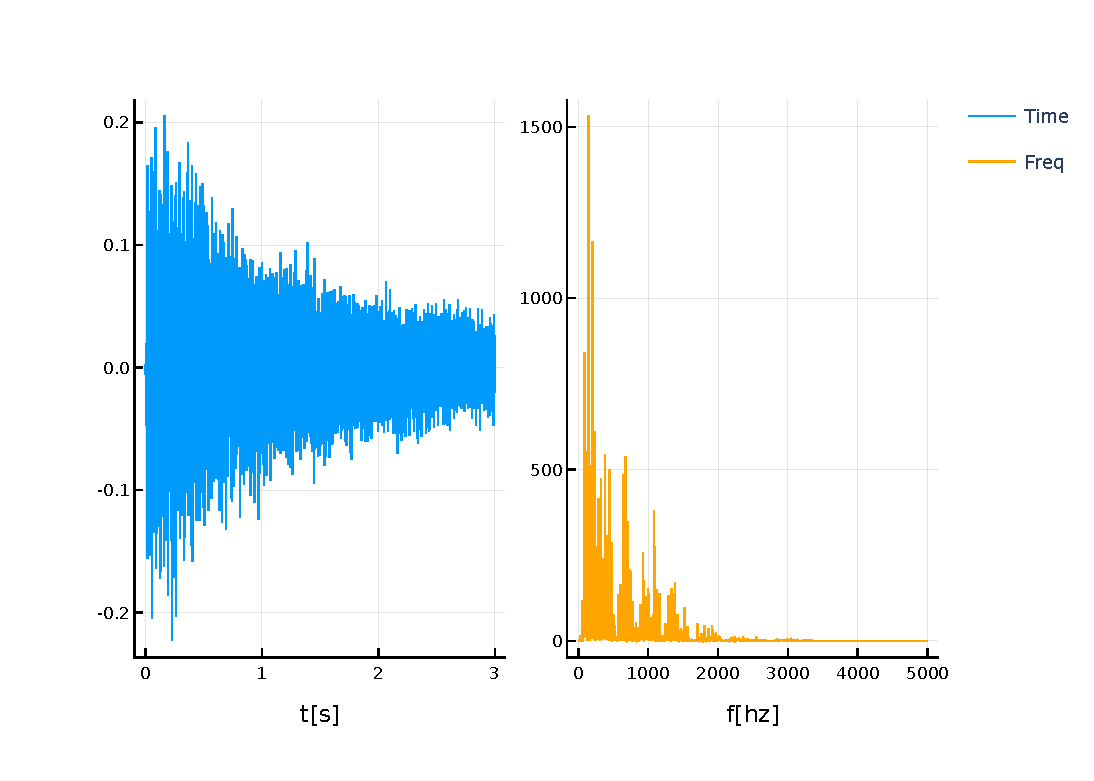
\includegraphics[width=1.0\linewidth]{assets/A1_sos.pdf}
		\caption{A\#1}
		\label{fig:a1_sos}
	\end{subfigure}%
	\begin{subfigure}{.5\textwidth}
		\centering
		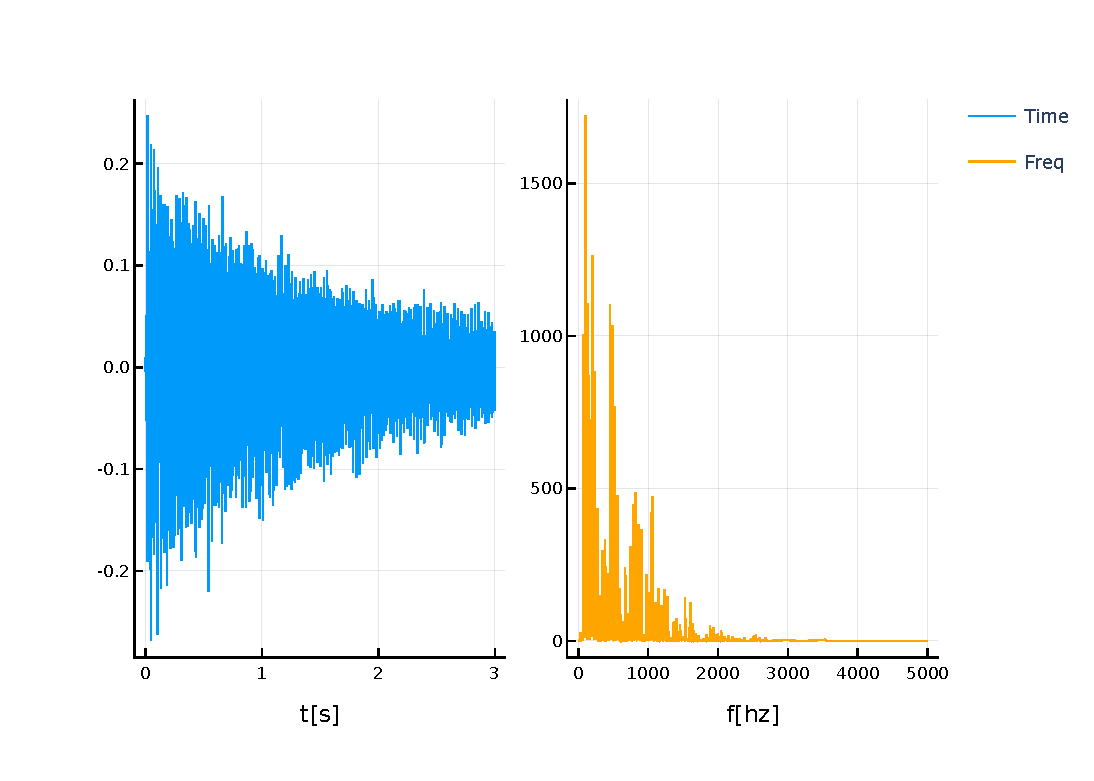
\includegraphics[width=1.0\linewidth]{assets/C1_sos.pdf}
		\caption{C\#1}
		\label{fig:c1_sos}
	\end{subfigure}
	\caption{}
\end{figure}

\begin{figure}[!ht]
	\centering
	\begin{subfigure}{.5\textwidth}
		\centering
		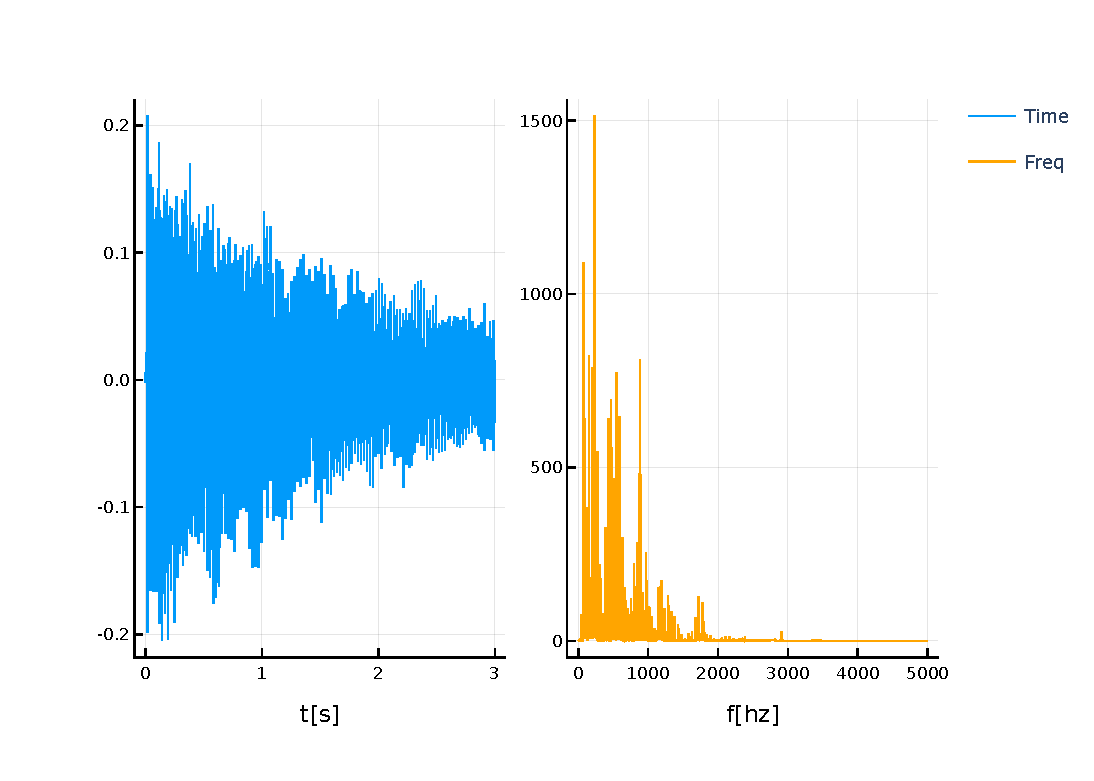
\includegraphics[width=1.0\linewidth]{assets/D1_sos.pdf}
		\caption{D\#1}
		\label{fig:d1_sos}
	\end{subfigure}%
	\begin{subfigure}{.5\textwidth}
		\centering
		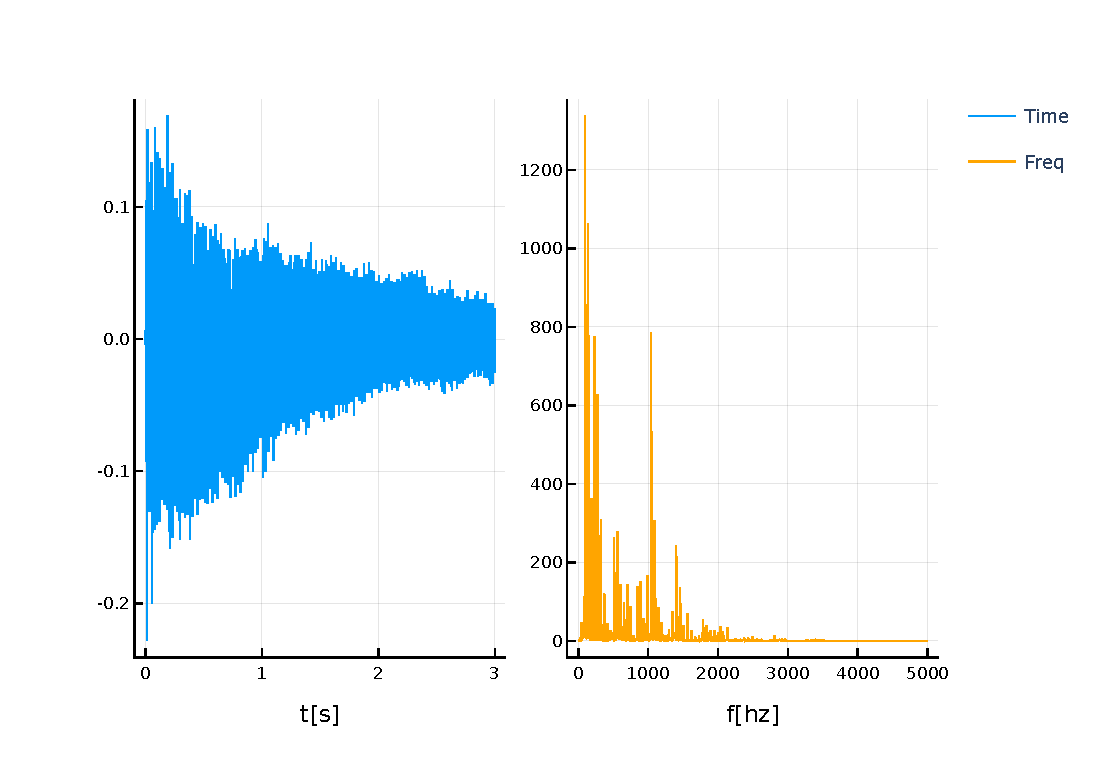
\includegraphics[width=1.0\linewidth]{assets/F1_sos.pdf}
		\caption{F\#1}
		\label{fig:f1_sos}
	\end{subfigure}
	\caption{}
\end{figure}

Se muestran a continuación los parámetros de normalización (volveremos a utilizar media cero) para cada característica en las Tablas \ref{Tab:Features_4_1},
\ref{Tab:Features_4_2} \ref{Tab:Features_4_3} y \ref{Tab:Features_4_4}.

\begin{table}
	\caption{Parámetros de normalización (I)}
	\centering
		\begin{tabular}{||c c c||}
			\hline
			Característica & Media & Desviación Típica \\ [0.5ex]
			\hline\hline
			E & $0.005290622$ & $0.009127998$ \\
			\hline
			zero-crossing & $3317.7852$ & $4477.6226$ \\
			\hline
			abs-max & $1445.9364$ & $1557.9128$ \\
			\hline
			abs-max-freq & $980.58826$ & $1027.9849$ \\
			\hline
			m\textsubscript{1} & $2.5213237$ & $4.892542$ \\
			\hline
			m\textsubscript{2} & $19.776129$ & $34.19082$ \\
			\hline
			m\textsubscript{3} & $18.500994$ & $33.448643$ \\
			\hline
			m\textsubscript{4} & $20.293629$ & $28.46877$ \\
			\hline
			m\textsubscript{5} & $15.832674$ & $24.200994$ \\
			\hline
			m\textsubscript{6} & $13.741416$ & $21.621166$ \\
			\hline
			m\textsubscript{7} & $13.71829$ & $20.745993$ \\
			\hline
			m\textsubscript{8} & $10.299257$ & $17.33558$ \\
			\hline
			m\textsubscript{9} & $9.490465$ & $18.469109$ \\
			\hline
			m\textsubscript{10} & $9.750799$ & $19.446434$ \\
			\hline
			m\textsubscript{11} & $9.340946$ & $13.882007$ \\
			\hline
			m\textsubscript{12} & $7.7851214$ & $11.177626$ \\
			\hline
			m\textsubscript{13} & $6.734947$ & $13.808262$ \\
			\hline
			m\textsubscript{14} & $5.5433474$ & $8.790224$ \\
			\hline
			m\textsubscript{15} & $4.2768292$ & $6.906526$ \\
			\hline
			m\textsubscript{16} & $4.459063$ & $7.8797054$ \\
			\hline
			m\textsubscript{17} & $2.9236934$ & $5.253287$ \\
			\hline
			m\textsubscript{18} & $2.6162808$ & $5.561383$ \\
			\hline
			m\textsubscript{19} & $2.5326357$ & $4.6802435$ \\
			\hline
			m\textsubscript{20} & $1.656642$ & $4.287465$ \\
			\hline
			m\textsubscript{21} & $1.6121823$ & $4.2043204$ \\
			\hline
			m\textsubscript{22} & $1.1647563$ & $3.044825$ \\
			\hline
			m\textsubscript{23} & $0.87163603$ & $2.4234502$ \\
			\hline
			m\textsubscript{24} & $0.83163273$ & $2.1765046$ \\
			\hline
			m\textsubscript{25} & $0.61601394$ & $1.4981358$ \\
			\hline
			m\textsubscript{26} & $0.5027224$ & $1.2157471$ \\
			\hline
			m\textsubscript{27} & $0.44925115$ & $1.2129601$ \\
			\hline
			m\textsubscript{28} & $0.3179743$ & $1.0582143$ \\
			\hline
			m\textsubscript{29} & $0.30106485$ & $1.2961926$ \\
			\hline
			m\textsubscript{30} & $0.12668554$ & $0.24906345$ \\
			\hline
		\end{tabular}
	\label{Tab:Features_4_1}
\end{table}

\begin{table}
	\caption{Parámetros de normalización (II)}
	\centering
		\begin{tabular}{||c c c||}
			\hline
			Característica & Media & Desviación Típica  \\ [0.5ex]
			\hline\hline
			std\textsubscript{1} & $3.7071$ & $8.894764$ \\
			\hline
			std\textsubscript{2} & $41.93409$ & $100.38277$ \\
			\hline
			std\textsubscript{3} & $41.496273$ & $100.46413$ \\
			\hline
			std\textsubscript{4} & $50.62945$ & $97.251366$ \\
			\hline
			std\textsubscript{5} & $32.27192$ & $66.25659$ \\
			\hline
			std\textsubscript{6} & $31.772036$ & $64.703476$ \\
			\hline
			std\textsubscript{7} & $30.200518$ & $56.291985$ \\
			\hline
			std\textsubscript{8} & $24.33468$ & $49.075897$ \\
			\hline
			std\textsubscript{9} & $17.22069$ & $40.07678$ \\
			\hline
			std\textsubscript{10} & $21.47563$ & $49.664173$ \\
			\hline
			std\textsubscript{11} & $16.356256$ & $32.295124$ \\
			\hline
			std\textsubscript{12} & $13.809475$ & $27.013056$ \\
			\hline
			std\textsubscript{13} & $13.494098$ & $35.255543$ \\
			\hline
			std\textsubscript{14} & $9.511233$ & $19.50926$ \\
			\hline
			std\textsubscript{15} & $7.4176326$ & $16.4802$ \\
			\hline
			std\textsubscript{16} & $7.555132$ & $18.873085$ \\
			\hline
			std\textsubscript{17} & $5.6317873$ & $11.938161$ \\
			\hline
			std\textsubscript{18} & $3.8923404$ & $10.900163$ \\
			\hline
			std\textsubscript{19} & $4.617325$ & $10.1336155$ \\
			\hline
			std\textsubscript{20} & $2.5670214$ & $8.334569$ \\
			\hline
			std\textsubscript{21} & $2.7792637$ & $7.7385535$ \\
			\hline
			std\textsubscript{22} & $1.8842899$ & $5.510914$ \\
			\hline
			std\textsubscript{23} & $1.4960651$ & $4.586712$ \\
			\hline
			std\textsubscript{24} & $1.4450701$ & $3.7847013$ \\
			\hline
			std\textsubscript{25} & $0.90402246$ & $2.5514781$ \\
			\hline
			std\textsubscript{26} & $0.7006507$ & $1.8386049$ \\
			\hline
			std\textsubscript{27} & $0.6376248$ & $1.6106461$ \\
			\hline
			std\textsubscript{28} & $0.48451066$ & $1.7358224$ \\
			\hline
			std\textsubscript{29} & $0.38622695$ & $1.3208534$ \\
			\hline
			std\textsubscript{30} & $0.18503572$ & $0.458966$ \\
			\hline
		\end{tabular}
	\label{Tab:Features_4_2}
\end{table}

\begin{table}
	\caption{Parámetros de normalización (III)}
	\centering
		\begin{tabular}{||c c c||}
			\hline
			Característica & Media & Desviación Típica  \\ [0.5ex]
			\hline\hline
			max\textsubscript{1} & $33.110157$ & $99.81226$ \\
			\hline
			max\textsubscript{2} & $415.37152$ & $1154.7861$ \\
			\hline
			max\textsubscript{3} & $422.34433$ & $1112.5609$ \\
			\hline
			max\textsubscript{4} & $536.3476$ & $1134.9387$ \\
			\hline
			max\textsubscript{5} & $317.401$ & $698.8781$ \\
			\hline
			max\textsubscript{6} & $316.10635$ & $644.3593$ \\
			\hline
			max\textsubscript{7} & $293.7506$ & $569.4251$ \\
			\hline
			max\textsubscript{8} & $239.86774$ & $471.9059$ \\
			\hline
			max\textsubscript{9} & $162.63959$ & $375.88123$ \\
			\hline
			max\textsubscript{10} & $207.69164$ & $447.70316$ \\
			\hline
			max\textsubscript{11} & $156.60005$ & $323.31445$ \\
			\hline
			max\textsubscript{12} & $132.93877$ & $264.18588$ \\
			\hline
			max\textsubscript{13} & $129.61961$ & $310.57278$ \\
			\hline
			max\textsubscript{14} & $90.64936$ & $186.6918$ \\
			\hline
			max\textsubscript{15} & $72.60896$ & $163.45084$ \\
			\hline
			max\textsubscript{16} & $68.42438$ & $165.54524$ \\
			\hline
			max\textsubscript{17} & $55.859993$ & $115.98919$ \\
			\hline
			max\textsubscript{18} & $35.653084$ & $97.61015$ \\
			\hline
			max\textsubscript{19} & $40.517826$ & $84.012886$ \\
			\hline
			max\textsubscript{20} & $22.404512$ & $67.51314$ \\
			\hline
			max\textsubscript{21} & $23.722889$ & $55.782883$ \\
			\hline
			max\textsubscript{22} & $16.067352$ & $41.516422$ \\
			\hline
			max\textsubscript{23} & $13.351332$ & $36.865856$ \\
			\hline
			max\textsubscript{24} & $11.76221$ & $26.125443$ \\
			\hline
			max\textsubscript{25} & $7.4373846$ & $19.201763$ \\
			\hline
			max\textsubscript{26} & $5.7013874$ & $14.642168$ \\
			\hline
			max\textsubscript{27} & $4.8674684$ & $10.794909$ \\
			\hline
			max\textsubscript{28} & $3.8479474$ & $11.645865$ \\
			\hline
			max\textsubscript{29} & $2.9212744$ & $8.312529$ \\
			\hline
			max\textsubscript{30} & $1.5820836$ & $3.9503338$ \\
			\hline
		\end{tabular}
	\label{Tab:Features_4_3}
\end{table}

\begin{table}
	\caption{Parámetros de normalización (IV)}
	\centering
		\begin{tabular}{||c c c||}
			\hline
			Característica & Media & Desviación Típica  \\ [0.5ex]
			\hline\hline
			max-freq\textsubscript{1} & $34.545124$ & $14.418398$ \\
			\hline
			max-freq\textsubscript{2} & $108.99156$ & $14.543035$ \\
			\hline
			max-freq\textsubscript{3} & $157.66272$ & $22.50655$ \\
			\hline
			max-freq\textsubscript{4} & $237.14865$ & $26.168978$ \\
			\hline
			max-freq\textsubscript{5} & $308.71167$ & $24.800741$ \\
			\hline
			max-freq\textsubscript{6} & $404.29333$ & $26.971804$ \\
			\hline
			max-freq\textsubscript{7} & $488.65253$ & $23.474133$ \\
			\hline
			max-freq\textsubscript{8} & $584.63116$ & $31.848839$ \\
			\hline
			max-freq\textsubscript{9} & $671.4978$ & $29.488453$ \\
			\hline
			max-freq\textsubscript{10} & $784.3489$ & $33.213223$ \\
			\hline
			max-freq\textsubscript{11} & $905.13873$ & $34.916843$ \\
			\hline
			max-freq\textsubscript{12} & $1005.73865$ & $39.89346$ \\
			\hline
			max-freq\textsubscript{13} & $1136.8329$ & $46.666904$ \\
			\hline
			max-freq\textsubscript{14} & $1264.4369$ & $42.46175$ \\
			\hline
			max-freq\textsubscript{15} & $1412.9193$ & $49.629932$ \\
			\hline
			max-freq\textsubscript{16} & $1537.3774$ & $44.49866$ \\
			\hline
			max-freq\textsubscript{17} & $1700.5549$ & $47.24032$ \\
			\hline
			max-freq\textsubscript{18} & $1871.9404$ & $52.69005$ \\
			\hline
			max-freq\textsubscript{19} & $2058.1985$ & $61.4545$ \\
			\hline
			max-freq\textsubscript{20} & $2220.4458$ & $62.312325$ \\
			\hline
			max-freq\textsubscript{21} & $2422.4363$ & $62.446247$ \\
			\hline
			max-freq\textsubscript{22} & $2629.6775$ & $65.41493$ \\
			\hline
			max-freq\textsubscript{23} & $2861.094$ & $72.73729$ \\
			\hline
			max-freq\textsubscript{24} & $3082.9204$ & $77.84288$ \\
			\hline
			max-freq\textsubscript{25} & $3346.068$ & $74.768135$ \\
			\hline
			max-freq\textsubscript{26} & $3592.8464$ & $87.46203$ \\
			\hline
			max-freq\textsubscript{27} & $3867.4265$ & $90.45616$ \\
			\hline
			max-freq\textsubscript{28} & $4171.0786$ & $102.07654$ \\
			\hline
			max-freq\textsubscript{29} & $4471.467$ & $94.344215$ \\
			\hline
			max-freq\textsubscript{30} & $4826.714$ & $102.89994$ \\
			\hline
		\end{tabular}
	\label{Tab:Features_4_4}
\end{table}

\newpage
\hphantom{skip}

Donde:
\begin{itemize}
	\item \textit{E} indica la \textbf{energía de la señal}.
	\item \textit{m\textsubscript{i}} indica la \textbf{media de la intensidad} en el intervalo \textit{i} en frecuencia.
	\item \textit{std\textsubscript{i}} indica la \textbf{desviación típica de la intensidad} en el intervalo \textit{i} en frecuencia.
	\item \textit{max\textsubscript{i}} indica el \textbf{máximo de la intensidad} en el intervalo \textit{i} en frecuencia.
	\item \textit{max-freq\textsubscript{i}} indica la \textbf{frecuencia donde se alcanza el máximo de intensidad} en el intervalo \textit{i} en frecuencia.
\end{itemize}

Para estos experimentos se volvió a repetir 20 veces el entrenamiento de la RNA en cada \textit{fold}, devolviendo el resultado promedio.

\bigskip
Utilizaremos de nuevo como medida el promedio del \textbf{F1-Score} en los \textit{folds}. Si hay empate en dicha media, se elegirá el modelo con menor
desviación típica de la métrica.

\subsubsection{Resultados}
Para permitir la reproducibilidad de los experimentos, se utilizó \textit{100} como semilla de generación de números
aleatorios.

\paragraph{RNA}

Para el entrenamiento de las RNA, se han utilizado los siguientes parámetros en común:
\begin{itemize}
	\item Ratio de aprendizaje: $0.01$
	\item Ratio de patrones para el conjunto de validación: $0.2$.
	\item Máximo número de ciclos (\textit{epochs}) de entrenamiento: $1500$.
	\item Máximo número de ciclos (\textit{epochs}) de entrenamiento sin mejorar el error de validación: $5$.
	\item Algoritmo de optimización: ADAM.
	\item Función de \textit{loss}: \textit{Cross Entropy}.
\end{itemize}
El hiperparámetro que hemos variado ha sido, de nuevo, la arquitectura de neuronas a utilizar, obteniendo 8 configuraciones diferentes.

Se muestran los resultados de la experimentación en la Tabla \ref{Tab:ANN_4}.

\begin{table}[!ht]
	\caption{Resultados RNA}
	\centering
		 \begin{tabular}{||c c c||}
			 \hline
			 Arquitectura & F1-Score & Precisión  \\ [0.5ex]
			 \hline\hline
			[16] & $0.95148 \pm 0.00551$ & $0.96105 \pm 0.00471$ \\
			\hline 
			[32] & $0.98759 \pm 0.00345$ & $0.9897 \pm 0.00221$ \\
			\hline 
			[64] & $0.99345 \pm 0.00309$ & $0.99428 \pm 0.00162$ \\
			\hline 
			[128] & $0.99293 \pm 0.00258$ & $0.99424 \pm 0.00123$ \\
			\hline 
			[256] & $0.99269 \pm 0.00345$ & $0.9936 \pm 0.00299$ \\
			\hline 
			[512] & $0.98348 \pm 0.0061$ & $0.98603 \pm 0.00423$ \\
			\hline 
			[64, 64] & $0.98322 \pm 0.00373$ & $0.98554 \pm 0.00292$ \\
			\hline 
			[64, 128] & $0.9818 \pm 0.00226$ & $0.98428 \pm 0.00227$ \\
			\hline 
		 \end{tabular}
	\label{Tab:ANN_4}
	\end{table}

\paragraph{SVM}

Para las máquinas de soporte vectorial hemos utilizado 8 configuraciones distintas de los hiperparámetros de \textit{kernel},
grado del \textit{kernel} (sólo se utiliza en \textit{kernel} polinomial), \textit{gamma} y \textit{C}.

Se muestran los resultados de la experimentación en la Tabla \ref{Tab:SVM_4}.

\newpage
\begin{table}[!ht]
	\caption{Resultados SVM}
	\centering
		 \begin{tabular}{||c c c||}
			\hline 
			(kernel, grado, gamma, C) & F1-Score & Precisión  \\ [0.5ex]  
			\hline\hline
			(poly, $3$, $1$, $1$) & $0.98957 \pm 0.00723$ & $0.9911 \pm 0.00594$ \\
			\hline 
			(rbf, $3$, $1$, $1$) & $0.08773 \pm 0.01527$ & $0.09143 \pm 0.01179$ \\
			\hline 
			(sigmoid, $3$, $1$, $1$) & $0.07182 \pm 0.00909$ & $0.1393 \pm 0.01431$ \\
			\hline 
			(poly, $3$, $10$, $0.1$) & $0.99152 \pm 0.00418$ & $0.99191 \pm 0.00394$ \\
			\hline 
			(rbf, $3$, $10$, $0.1$) & $0.00068 \pm 3.0e-5$ & $0.02965 \pm 0.00136$ \\
			\hline 
			(rbf, $3$, $0.001$, $100$) & $0.99605 \pm 0.00408$ & $0.99612 \pm 0.00324$ \\
			\hline 
			(rbf, $3$, $0.01$, $100$) & $0.9947 \pm 0.00389$ & $0.99459 \pm 0.00313$ \\
			\hline 
			(poly, $3$, $100$, $0.001$) & $0.99142 \pm 0.00449$ & $0.99237 \pm 0.00367$ \\
			\hline 
		 \end{tabular}
	\label{Tab:SVM_4}
	\end{table}

\paragraph{Árboles de decisión}
Para los árboles de decisión hemos utilizado 6 configuraciones distintas del hiperparámetro de profundidad máxima.

Se muestran los resultados de la experimentación en la Tabla \ref{Tab:DecisionTree_4}.

\begin{table}[!ht]
	\caption{Resultados Árbol de decisión}
	\centering
		 \begin{tabular}{||c c c||}
			\hline 
			Altura máxima & F1-Score & Precisión  \\ [0.5ex]  
			\hline\hline
			$32$ & $0.93688 \pm 0.0118$ & $0.94355 \pm 0.00995$ \\
			\hline 
			$64$ & $0.92919 \pm 0.01756$ & $0.93871 \pm 0.01425$ \\
			\hline 
			$128$ & $0.92578 \pm 0.02024$ & $0.93693 \pm 0.01502$ \\
			\hline 
			$256$ & $0.93336 \pm 0.01516$ & $0.94104 \pm 0.01578$ \\
			\hline 
			$512$ & $0.93528 \pm 0.01411$ & $0.9438 \pm 0.01019$ \\
			\hline 
			$1024$ & $0.93482 \pm 0.01642$ & $0.94221 \pm 0.01563$ \\
			\hline
		 \end{tabular}
	\label{Tab:DecisionTree_4}
	\end{table}

\paragraph{kNN}
Para el modelo kNN hemos utilizado 6 configuraciones distintas del hiperparámetro de k (número de vecinos más cercanos).

Se muestran los resultados de la experimentación en la tabla \ref{Tab:kNN_4}.

\begin{table}[!ht]
	\caption{Resultados kNN}
	\centering
		\begin{tabular}{||c c c||}
			\hline 
			K & F1-Score & Precisión  \\ [0.5ex]  
			\hline\hline
			$2$ & $0.98126 \pm 0.00699$ & $0.98422 \pm 0.00492$ \\
			\hline 
			$3$ & $0.98306 \pm 0.00593$ & $0.98473 \pm 0.00477$ \\
			\hline 
			$7$ & $0.97125 \pm 0.00862$ & $0.9767 \pm 0.00708$ \\
			\hline 
			$15$ & $0.95195 \pm 0.01088$ & $0.96343 \pm 0.00783$ \\
			\hline 
			$31$ & $0.93762 \pm 0.01577$ & $0.95012 \pm 0.01025$ \\
			\hline 
			$63$ & $0.88327 \pm 0.01502$ & $0.91107 \pm 0.00954$ \\
			\hline 
		\end{tabular}
	\label{Tab:kNN_4}
\end{table}

\subsubsection{Discusión}

Como se puede ver en los resultados, el funcionamiento de nuestro sistema resolviendo el problema completo, es decir, clasificando todas las notas
del piano, es sorprendente. Con el mejor modelo (de nuevo un SVM), obtuvimos una precisión de $0.99538$ ± $0.00197$ y un F1-Score de $0.9956$ ± $0.0026$,
haciendo uso de un \textit{kernel} de base radial, un valor de \textit{gamma} $0.01$ y un valor de \textit{C} $100$.

\bigskip
De nuevo destacar que, a pesar de obtener RNAs con valores de F1-Score muy altos (\textgreater99\%), el tiempo invertido en el entrenamiento las
hace modelos menos interesantes, sobre todo comparados con los modelos basados en SVM o kNN.

\bigskip
Con respecto a las características, creemos que tanto la \textbf{frecuencia máxima absoluta} y la \textbf{itensidad máxima absoluta en frecuencia},
son importantes a la hora de clasificar correctamente las notas. Sin embargo, ahora que tenemos el problema completo resuelto, consideramos que
es el momento de tratar de minimizar el número de características necesarias, perdiendo la menor precisión en la clasificación posible.
Este aspecto será en el que nos centremos en la siguiente aproximación.

\bigskip
Se muestra en la Tabla \ref{tab:confusion_matrix_4} la matriz de confusión del mejor modelo obtenido, puediendo observar como se
confunde mayoritariamente en notas que se encuentran a distancias cercanas como son \textit{A5} y \textit{A\#5} o \textit{F7} y \textit{G7}. 

\begin{table}[!ht]
	\centering
	% \begin{turn}{90}

	\resizebox{\textwidth}{!}{
		\begin{tabular}{cccccccccccccccccccccccccccccccccccccc}
			&                          & \multicolumn{36}{c}{Predicc.}                                                                                                                                                                                                                                                                                                                                                                                                                                                                                                                                                                                                                                                                                                                                                                                                                                                                                                                                                                                                                 \\ \cline{3-38} 
			& \multicolumn{1}{c|}{}    & \multicolumn{1}{c|}{C1} & \multicolumn{1}{c|}{C2} & \multicolumn{1}{c|}{C3} & \multicolumn{1}{c|}{C4} & \multicolumn{1}{c|}{C5} & \multicolumn{1}{c|}{C6} & \multicolumn{1}{c|}{C7} & \multicolumn{1}{c|}{C8} & \multicolumn{1}{c|}{A1} & \multicolumn{1}{c|}{A2} & \multicolumn{1}{c|}{...}                  & \multicolumn{1}{c|}{B4} & \multicolumn{1}{c|}{B5} & \multicolumn{1}{c|}{B6} & \multicolumn{1}{c|}{B7} & \multicolumn{1}{c|}{D1} & \multicolumn{1}{c|}{...}                  & \multicolumn{1}{c|}{E1} & \multicolumn{1}{c|}{E2} & \multicolumn{1}{c|}{E3} & \multicolumn{1}{c|}{...}                  & \multicolumn{1}{c|}{E6} & \multicolumn{1}{c|}{E7} & \multicolumn{1}{c|}{F1} & \multicolumn{1}{c|}{F2} & \multicolumn{1}{c|}{F3} & \multicolumn{1}{c|}{...}                  & \multicolumn{1}{c|}{F6} & \multicolumn{1}{c|}{F7} & \multicolumn{1}{c|}{G1} & \multicolumn{1}{c|}{G2} & \multicolumn{1}{c|}{G3} & \multicolumn{1}{c|}{G4} & \multicolumn{1}{c|}{G5} & \multicolumn{1}{c|}{G6} & \multicolumn{1}{c|}{G7} \\ \cline{2-38} 
\multicolumn{1}{c|}{\multirow{22}{*}{Real}} & \multicolumn{1}{c|}{C1}  & \multicolumn{1}{c|}{7}  & \multicolumn{1}{c|}{0}  & \multicolumn{1}{c|}{0}  & \multicolumn{1}{c|}{0}  & \multicolumn{1}{c|}{0}  & \multicolumn{1}{c|}{0}  & \multicolumn{1}{c|}{0}  & \multicolumn{1}{c|}{0}  & \multicolumn{1}{c|}{0}  & \multicolumn{1}{c|}{0}  & \multicolumn{1}{c|}{\multirow{5}{*}{,,,}} & \multicolumn{1}{c|}{0}  & \multicolumn{1}{c|}{0}  & \multicolumn{1}{c|}{0}  & \multicolumn{1}{c|}{0}  & \multicolumn{1}{c|}{0}  & \multicolumn{1}{c|}{\multirow{5}{*}{,,,}} & \multicolumn{1}{c|}{0}  & \multicolumn{1}{c|}{0}  & \multicolumn{1}{c|}{0}  & \multicolumn{1}{c|}{\multirow{5}{*}{,,,}} & \multicolumn{1}{c|}{0}  & \multicolumn{1}{c|}{0}  & \multicolumn{1}{c|}{0}  & \multicolumn{1}{c|}{0}  & \multicolumn{1}{c|}{0}  & \multicolumn{1}{c|}{\multirow{5}{*}{,,,}} & \multicolumn{1}{c|}{0}  & \multicolumn{1}{c|}{0}  & \multicolumn{1}{c|}{0}  & \multicolumn{1}{c|}{0}  & \multicolumn{1}{c|}{0}  & \multicolumn{1}{c|}{0}  & \multicolumn{1}{c|}{0}  & \multicolumn{1}{c|}{0}  & \multicolumn{1}{c|}{0}  \\ \cline{2-12} \cline{14-18} \cline{20-22} \cline{24-28} \cline{30-38} 
\multicolumn{1}{c|}{}                       & \multicolumn{1}{c|}{C2}  & \multicolumn{1}{c|}{0}  & \multicolumn{1}{c|}{7}  & \multicolumn{1}{c|}{0}  & \multicolumn{1}{c|}{0}  & \multicolumn{1}{c|}{0}  & \multicolumn{1}{c|}{0}  & \multicolumn{1}{c|}{0}  & \multicolumn{1}{c|}{0}  & \multicolumn{1}{c|}{0}  & \multicolumn{1}{c|}{0}  & \multicolumn{1}{c|}{}                     & \multicolumn{1}{c|}{0}  & \multicolumn{1}{c|}{0}  & \multicolumn{1}{c|}{0}  & \multicolumn{1}{c|}{0}  & \multicolumn{1}{c|}{0}  & \multicolumn{1}{c|}{}                     & \multicolumn{1}{c|}{0}  & \multicolumn{1}{c|}{0}  & \multicolumn{1}{c|}{0}  & \multicolumn{1}{c|}{}                     & \multicolumn{1}{c|}{0}  & \multicolumn{1}{c|}{0}  & \multicolumn{1}{c|}{0}  & \multicolumn{1}{c|}{0}  & \multicolumn{1}{c|}{0}  & \multicolumn{1}{c|}{}                     & \multicolumn{1}{c|}{0}  & \multicolumn{1}{c|}{0}  & \multicolumn{1}{c|}{0}  & \multicolumn{1}{c|}{0}  & \multicolumn{1}{c|}{0}  & \multicolumn{1}{c|}{0}  & \multicolumn{1}{c|}{0}  & \multicolumn{1}{c|}{0}  & \multicolumn{1}{c|}{0}  \\ \cline{2-12} \cline{14-18} \cline{20-22} \cline{24-28} \cline{30-38} 
\multicolumn{1}{c|}{}                       & \multicolumn{1}{c|}{C3}  & \multicolumn{1}{c|}{0}  & \multicolumn{1}{c|}{0}  & \multicolumn{1}{c|}{11} & \multicolumn{1}{c|}{0}  & \multicolumn{1}{c|}{0}  & \multicolumn{1}{c|}{0}  & \multicolumn{1}{c|}{0}  & \multicolumn{1}{c|}{0}  & \multicolumn{1}{c|}{0}  & \multicolumn{1}{c|}{0}  & \multicolumn{1}{c|}{}                     & \multicolumn{1}{c|}{0}  & \multicolumn{1}{c|}{0}  & \multicolumn{1}{c|}{0}  & \multicolumn{1}{c|}{0}  & \multicolumn{1}{c|}{0}  & \multicolumn{1}{c|}{}                     & \multicolumn{1}{c|}{0}  & \multicolumn{1}{c|}{0}  & \multicolumn{1}{c|}{0}  & \multicolumn{1}{c|}{}                     & \multicolumn{1}{c|}{0}  & \multicolumn{1}{c|}{0}  & \multicolumn{1}{c|}{0}  & \multicolumn{1}{c|}{0}  & \multicolumn{1}{c|}{0}  & \multicolumn{1}{c|}{}                     & \multicolumn{1}{c|}{0}  & \multicolumn{1}{c|}{0}  & \multicolumn{1}{c|}{0}  & \multicolumn{1}{c|}{0}  & \multicolumn{1}{c|}{0}  & \multicolumn{1}{c|}{0}  & \multicolumn{1}{c|}{0}  & \multicolumn{1}{c|}{0}  & \multicolumn{1}{c|}{0}  \\ \cline{2-12} \cline{14-18} \cline{20-22} \cline{24-28} \cline{30-38} 
\multicolumn{1}{c|}{}                       & \multicolumn{1}{c|}{C4}  & \multicolumn{1}{c|}{0}  & \multicolumn{1}{c|}{0}  & \multicolumn{1}{c|}{0}  & \multicolumn{1}{c|}{15} & \multicolumn{1}{c|}{0}  & \multicolumn{1}{c|}{0}  & \multicolumn{1}{c|}{0}  & \multicolumn{1}{c|}{0}  & \multicolumn{1}{c|}{0}  & \multicolumn{1}{c|}{0}  & \multicolumn{1}{c|}{}                     & \multicolumn{1}{c|}{0}  & \multicolumn{1}{c|}{0}  & \multicolumn{1}{c|}{0}  & \multicolumn{1}{c|}{0}  & \multicolumn{1}{c|}{0}  & \multicolumn{1}{c|}{}                     & \multicolumn{1}{c|}{0}  & \multicolumn{1}{c|}{0}  & \multicolumn{1}{c|}{0}  & \multicolumn{1}{c|}{}                     & \multicolumn{1}{c|}{0}  & \multicolumn{1}{c|}{0}  & \multicolumn{1}{c|}{0}  & \multicolumn{1}{c|}{0}  & \multicolumn{1}{c|}{0}  & \multicolumn{1}{c|}{}                     & \multicolumn{1}{c|}{0}  & \multicolumn{1}{c|}{0}  & \multicolumn{1}{c|}{0}  & \multicolumn{1}{c|}{0}  & \multicolumn{1}{c|}{0}  & \multicolumn{1}{c|}{0}  & \multicolumn{1}{c|}{0}  & \multicolumn{1}{c|}{0}  & \multicolumn{1}{c|}{0}  \\ \cline{2-12} \cline{14-18} \cline{20-22} \cline{24-28} \cline{30-38} 
\multicolumn{1}{c|}{}                       & \multicolumn{1}{c|}{C5}  & \multicolumn{1}{c|}{0}  & \multicolumn{1}{c|}{0}  & \multicolumn{1}{c|}{0}  & \multicolumn{1}{c|}{0}  & \multicolumn{1}{c|}{32} & \multicolumn{1}{c|}{0}  & \multicolumn{1}{c|}{0}  & \multicolumn{1}{c|}{0}  & \multicolumn{1}{c|}{0}  & \multicolumn{1}{c|}{0}  & \multicolumn{1}{c|}{}                     & \multicolumn{1}{c|}{0}  & \multicolumn{1}{c|}{0}  & \multicolumn{1}{c|}{0}  & \multicolumn{1}{c|}{0}  & \multicolumn{1}{c|}{0}  & \multicolumn{1}{c|}{}                     & \multicolumn{1}{c|}{0}  & \multicolumn{1}{c|}{0}  & \multicolumn{1}{c|}{0}  & \multicolumn{1}{c|}{}                     & \multicolumn{1}{c|}{0}  & \multicolumn{1}{c|}{0}  & \multicolumn{1}{c|}{0}  & \multicolumn{1}{c|}{0}  & \multicolumn{1}{c|}{0}  & \multicolumn{1}{c|}{}                     & \multicolumn{1}{c|}{0}  & \multicolumn{1}{c|}{0}  & \multicolumn{1}{c|}{0}  & \multicolumn{1}{c|}{0}  & \multicolumn{1}{c|}{0}  & \multicolumn{1}{c|}{0}  & \multicolumn{1}{c|}{0}  & \multicolumn{1}{c|}{0}  & \multicolumn{1}{c|}{0}  \\ \cline{2-12} \cline{14-18} \cline{20-22} \cline{24-28} \cline{30-38} 
\multicolumn{1}{c|}{}                       & \multicolumn{1}{c|}{...} & \multicolumn{36}{c|}{...}                                                                                                                                                                                                                                                                                                                                                                                                                                                                                                                                                                                                                                                                                                                                                                                                                                                                                                                                                                                                                     \\ \cline{2-12} \cline{14-18} \cline{20-22} \cline{24-28} \cline{30-38} 
\multicolumn{1}{c|}{}                       & \multicolumn{1}{c|}{B5}  & \multicolumn{1}{c|}{0}  & \multicolumn{1}{c|}{0}  & \multicolumn{1}{c|}{0}  & \multicolumn{1}{c|}{0}  & \multicolumn{1}{c|}{0}  & \multicolumn{1}{c|}{0}  & \multicolumn{1}{c|}{0}  & \multicolumn{1}{c|}{0}  & \multicolumn{1}{c|}{0}  & \multicolumn{1}{c|}{0}  & \multicolumn{1}{c|}{\multirow{3}{*}{...}} & \multicolumn{1}{c|}{0}  & \multicolumn{1}{c|}{14} & \multicolumn{1}{c|}{0}  & \multicolumn{1}{c|}{0}  & \multicolumn{1}{c|}{0}  & \multicolumn{1}{c|}{\multirow{3}{*}{...}} & \multicolumn{1}{c|}{0}  & \multicolumn{1}{c|}{0}  & \multicolumn{1}{c|}{0}  & \multicolumn{1}{c|}{\multirow{3}{*}{...}} & \multicolumn{1}{c|}{0}  & \multicolumn{1}{c|}{0}  & \multicolumn{1}{c|}{0}  & \multicolumn{1}{c|}{0}  & \multicolumn{1}{c|}{0}  & \multicolumn{1}{c|}{\multirow{3}{*}{...}} & \multicolumn{1}{c|}{0}  & \multicolumn{1}{c|}{0}  & \multicolumn{1}{c|}{0}  & \multicolumn{1}{c|}{0}  & \multicolumn{1}{c|}{0}  & \multicolumn{1}{c|}{0}  & \multicolumn{1}{c|}{0}  & \multicolumn{1}{c|}{0}  & \multicolumn{1}{c|}{0}  \\ \cline{2-12} \cline{14-18} \cline{20-22} \cline{24-28} \cline{30-38} 
\multicolumn{1}{c|}{}                       & \multicolumn{1}{c|}{B6}  & \multicolumn{1}{c|}{0}  & \multicolumn{1}{c|}{0}  & \multicolumn{1}{c|}{0}  & \multicolumn{1}{c|}{0}  & \multicolumn{1}{c|}{0}  & \multicolumn{1}{c|}{0}  & \multicolumn{1}{c|}{0}  & \multicolumn{1}{c|}{1}  & \multicolumn{1}{c|}{0}  & \multicolumn{1}{c|}{0}  & \multicolumn{1}{c|}{}                     & \multicolumn{1}{c|}{0}  & \multicolumn{1}{c|}{0}  & \multicolumn{1}{c|}{18} & \multicolumn{1}{c|}{0}  & \multicolumn{1}{c|}{0}  & \multicolumn{1}{c|}{}                     & \multicolumn{1}{c|}{0}  & \multicolumn{1}{c|}{0}  & \multicolumn{1}{c|}{0}  & \multicolumn{1}{c|}{}                     & \multicolumn{1}{c|}{0}  & \multicolumn{1}{c|}{0}  & \multicolumn{1}{c|}{0}  & \multicolumn{1}{c|}{0}  & \multicolumn{1}{c|}{0}  & \multicolumn{1}{c|}{}                     & \multicolumn{1}{c|}{0}  & \multicolumn{1}{c|}{0}  & \multicolumn{1}{c|}{0}  & \multicolumn{1}{c|}{0}  & \multicolumn{1}{c|}{0}  & \multicolumn{1}{c|}{0}  & \multicolumn{1}{c|}{0}  & \multicolumn{1}{c|}{0}  & \multicolumn{1}{c|}{0}  \\ \cline{2-12} \cline{14-18} \cline{20-22} \cline{24-28} \cline{30-38} 
\multicolumn{1}{c|}{}                       & \multicolumn{1}{c|}{B7}  & \multicolumn{1}{c|}{0}  & \multicolumn{1}{c|}{0}  & \multicolumn{1}{c|}{0}  & \multicolumn{1}{c|}{0}  & \multicolumn{1}{c|}{0}  & \multicolumn{1}{c|}{0}  & \multicolumn{1}{c|}{0}  & \multicolumn{1}{c|}{0}  & \multicolumn{1}{c|}{0}  & \multicolumn{1}{c|}{0}  & \multicolumn{1}{c|}{}                     & \multicolumn{1}{c|}{0}  & \multicolumn{1}{c|}{0}  & \multicolumn{1}{c|}{0}  & \multicolumn{1}{c|}{14} & \multicolumn{1}{c|}{0}  & \multicolumn{1}{c|}{}                     & \multicolumn{1}{c|}{0}  & \multicolumn{1}{c|}{0}  & \multicolumn{1}{c|}{0}  & \multicolumn{1}{c|}{}                     & \multicolumn{1}{c|}{0}  & \multicolumn{1}{c|}{0}  & \multicolumn{1}{c|}{0}  & \multicolumn{1}{c|}{0}  & \multicolumn{1}{c|}{0}  & \multicolumn{1}{c|}{}                     & \multicolumn{1}{c|}{0}  & \multicolumn{1}{c|}{0}  & \multicolumn{1}{c|}{0}  & \multicolumn{1}{c|}{0}  & \multicolumn{1}{c|}{0}  & \multicolumn{1}{c|}{0}  & \multicolumn{1}{c|}{0}  & \multicolumn{1}{c|}{0}  & \multicolumn{1}{c|}{0}  \\ \cline{2-12} \cline{14-18} \cline{20-22} \cline{24-28} \cline{30-38} 
\multicolumn{1}{c|}{}                       & \multicolumn{1}{c|}{...} & \multicolumn{36}{c|}{...}                                                                                                                                                                                                                                                                                                                                                                                                                                                                                                                                                                                                                                                                                                                                                                                                                                                                                                                                                                                                                     \\ \cline{2-12} \cline{14-18} \cline{20-22} \cline{24-28} \cline{30-38} 
\multicolumn{1}{c|}{}                       & \multicolumn{1}{c|}{E7}  & \multicolumn{1}{c|}{0}  & \multicolumn{1}{c|}{0}  & \multicolumn{1}{c|}{0}  & \multicolumn{1}{c|}{0}  & \multicolumn{1}{c|}{0}  & \multicolumn{1}{c|}{0}  & \multicolumn{1}{c|}{0}  & \multicolumn{1}{c|}{0}  & \multicolumn{1}{c|}{0}  & \multicolumn{1}{c|}{0}  & \multicolumn{1}{c|}{\multirow{3}{*}{...}} & \multicolumn{1}{c|}{0}  & \multicolumn{1}{c|}{0}  & \multicolumn{1}{c|}{0}  & \multicolumn{1}{c|}{0}  & \multicolumn{1}{c|}{0}  & \multicolumn{1}{c|}{\multirow{3}{*}{...}} & \multicolumn{1}{c|}{0}  & \multicolumn{1}{c|}{0}  & \multicolumn{1}{c|}{0}  & \multicolumn{1}{c|}{\multirow{3}{*}{..}}  & \multicolumn{1}{c|}{0}  & \multicolumn{1}{c|}{17} & \multicolumn{1}{c|}{0}  & \multicolumn{1}{c|}{0}  & \multicolumn{1}{c|}{0}  & \multicolumn{1}{c|}{\multirow{3}{*}{...}} & \multicolumn{1}{c|}{0}  & \multicolumn{1}{c|}{0}  & \multicolumn{1}{c|}{0}  & \multicolumn{1}{c|}{0}  & \multicolumn{1}{c|}{0}  & \multicolumn{1}{c|}{0}  & \multicolumn{1}{c|}{0}  & \multicolumn{1}{c|}{0}  & \multicolumn{1}{c|}{0}  \\ \cline{2-12} \cline{14-18} \cline{20-22} \cline{24-28} \cline{30-38} 
\multicolumn{1}{c|}{}                       & \multicolumn{1}{c|}{F1}  & \multicolumn{1}{c|}{0}  & \multicolumn{1}{c|}{0}  & \multicolumn{1}{c|}{0}  & \multicolumn{1}{c|}{0}  & \multicolumn{1}{c|}{0}  & \multicolumn{1}{c|}{0}  & \multicolumn{1}{c|}{0}  & \multicolumn{1}{c|}{0}  & \multicolumn{1}{c|}{2}  & \multicolumn{1}{c|}{0}  & \multicolumn{1}{c|}{}                     & \multicolumn{1}{c|}{0}  & \multicolumn{1}{c|}{0}  & \multicolumn{1}{c|}{0}  & \multicolumn{1}{c|}{0}  & \multicolumn{1}{c|}{0}  & \multicolumn{1}{c|}{}                     & \multicolumn{1}{c|}{0}  & \multicolumn{1}{c|}{0}  & \multicolumn{1}{c|}{0}  & \multicolumn{1}{c|}{}                     & \multicolumn{1}{c|}{0}  & \multicolumn{1}{c|}{0}  & \multicolumn{1}{c|}{4}  & \multicolumn{1}{c|}{0}  & \multicolumn{1}{c|}{0}  & \multicolumn{1}{c|}{}                     & \multicolumn{1}{c|}{0}  & \multicolumn{1}{c|}{0}  & \multicolumn{1}{c|}{0}  & \multicolumn{1}{c|}{0}  & \multicolumn{1}{c|}{0}  & \multicolumn{1}{c|}{0}  & \multicolumn{1}{c|}{0}  & \multicolumn{1}{c|}{0}  & \multicolumn{1}{c|}{0}  \\ \cline{2-12} \cline{14-18} \cline{20-22} \cline{24-28} \cline{30-38} 
\multicolumn{1}{c|}{}                       & \multicolumn{1}{c|}{F2}  & \multicolumn{1}{c|}{0}  & \multicolumn{1}{c|}{0}  & \multicolumn{1}{c|}{0}  & \multicolumn{1}{c|}{0}  & \multicolumn{1}{c|}{0}  & \multicolumn{1}{c|}{0}  & \multicolumn{1}{c|}{0}  & \multicolumn{1}{c|}{0}  & \multicolumn{1}{c|}{0}  & \multicolumn{1}{c|}{0}  & \multicolumn{1}{c|}{}                     & \multicolumn{1}{c|}{0}  & \multicolumn{1}{c|}{0}  & \multicolumn{1}{c|}{0}  & \multicolumn{1}{c|}{0}  & \multicolumn{1}{c|}{0}  & \multicolumn{1}{c|}{}                     & \multicolumn{1}{c|}{0}  & \multicolumn{1}{c|}{0}  & \multicolumn{1}{c|}{0}  & \multicolumn{1}{c|}{}                     & \multicolumn{1}{c|}{0}  & \multicolumn{1}{c|}{0}  & \multicolumn{1}{c|}{0}  & \multicolumn{1}{c|}{12} & \multicolumn{1}{c|}{0}  & \multicolumn{1}{c|}{}                     & \multicolumn{1}{c|}{0}  & \multicolumn{1}{c|}{0}  & \multicolumn{1}{c|}{0}  & \multicolumn{1}{c|}{0}  & \multicolumn{1}{c|}{0}  & \multicolumn{1}{c|}{0}  & \multicolumn{1}{c|}{0}  & \multicolumn{1}{c|}{0}  & \multicolumn{1}{c|}{0}  \\ \cline{2-12} \cline{14-18} \cline{20-22} \cline{24-28} \cline{30-38} 
\multicolumn{1}{c|}{}                       & \multicolumn{1}{c|}{...} & \multicolumn{36}{c|}{...}                                                                                                                                                                                                                                                                                                                                                                                                                                                                                                                                                                                                                                                                                                                                                                                                                                                                                                                                                                                                                     \\ \cline{2-12} \cline{14-18} \cline{20-22} \cline{24-28} \cline{30-38} 
\multicolumn{1}{c|}{}                       & \multicolumn{1}{c|}{F7}  & \multicolumn{1}{c|}{0}  & \multicolumn{1}{c|}{0}  & \multicolumn{1}{c|}{0}  & \multicolumn{1}{c|}{0}  & \multicolumn{1}{c|}{0}  & \multicolumn{1}{c|}{0}  & \multicolumn{1}{c|}{0}  & \multicolumn{1}{c|}{0}  & \multicolumn{1}{c|}{0}  & \multicolumn{1}{c|}{0}  & \multicolumn{1}{c|}{\multirow{8}{*}{...}} & \multicolumn{1}{c|}{0}  & \multicolumn{1}{c|}{0}  & \multicolumn{1}{c|}{0}  & \multicolumn{1}{c|}{0}  & \multicolumn{1}{c|}{0}  & \multicolumn{1}{c|}{\multirow{8}{*}{...}} & \multicolumn{1}{c|}{0}  & \multicolumn{1}{c|}{0}  & \multicolumn{1}{c|}{0}  & \multicolumn{1}{c|}{\multirow{8}{*}{...}} & \multicolumn{1}{c|}{0}  & \multicolumn{1}{c|}{0}  & \multicolumn{1}{c|}{0}  & \multicolumn{1}{c|}{0}  & \multicolumn{1}{c|}{0}  & \multicolumn{1}{c|}{\multirow{8}{*}{...}} & \multicolumn{1}{c|}{0}  & \multicolumn{1}{c|}{15} & \multicolumn{1}{c|}{0}  & \multicolumn{1}{c|}{0}  & \multicolumn{1}{c|}{0}  & \multicolumn{1}{c|}{0}  & \multicolumn{1}{c|}{0}  & \multicolumn{1}{c|}{0}  & \multicolumn{1}{c|}{0}  \\ \cline{2-12} \cline{14-18} \cline{20-22} \cline{24-28} \cline{30-38} 
\multicolumn{1}{c|}{}                       & \multicolumn{1}{c|}{G1}  & \multicolumn{1}{c|}{0}  & \multicolumn{1}{c|}{0}  & \multicolumn{1}{c|}{0}  & \multicolumn{1}{c|}{0}  & \multicolumn{1}{c|}{0}  & \multicolumn{1}{c|}{0}  & \multicolumn{1}{c|}{0}  & \multicolumn{1}{c|}{0}  & \multicolumn{1}{c|}{3}  & \multicolumn{1}{c|}{0}  & \multicolumn{1}{c|}{}                     & \multicolumn{1}{c|}{0}  & \multicolumn{1}{c|}{0}  & \multicolumn{1}{c|}{0}  & \multicolumn{1}{c|}{0}  & \multicolumn{1}{c|}{0}  & \multicolumn{1}{c|}{}                     & \multicolumn{1}{c|}{0}  & \multicolumn{1}{c|}{1}  & \multicolumn{1}{c|}{0}  & \multicolumn{1}{c|}{}                     & \multicolumn{1}{c|}{0}  & \multicolumn{1}{c|}{0}  & \multicolumn{1}{c|}{0}  & \multicolumn{1}{c|}{0}  & \multicolumn{1}{c|}{0}  & \multicolumn{1}{c|}{}                     & \multicolumn{1}{c|}{0}  & \multicolumn{1}{c|}{0}  & \multicolumn{1}{c|}{5}  & \multicolumn{1}{c|}{0}  & \multicolumn{1}{c|}{0}  & \multicolumn{1}{c|}{0}  & \multicolumn{1}{c|}{0}  & \multicolumn{1}{c|}{0}  & \multicolumn{1}{c|}{0}  \\ \cline{2-12} \cline{14-18} \cline{20-22} \cline{24-28} \cline{30-38} 
\multicolumn{1}{c|}{}                       & \multicolumn{1}{c|}{G2}  & \multicolumn{1}{c|}{0}  & \multicolumn{1}{c|}{0}  & \multicolumn{1}{c|}{0}  & \multicolumn{1}{c|}{0}  & \multicolumn{1}{c|}{0}  & \multicolumn{1}{c|}{0}  & \multicolumn{1}{c|}{0}  & \multicolumn{1}{c|}{0}  & \multicolumn{1}{c|}{0}  & \multicolumn{1}{c|}{0}  & \multicolumn{1}{c|}{}                     & \multicolumn{1}{c|}{0}  & \multicolumn{1}{c|}{0}  & \multicolumn{1}{c|}{0}  & \multicolumn{1}{c|}{0}  & \multicolumn{1}{c|}{0}  & \multicolumn{1}{c|}{}                     & \multicolumn{1}{c|}{0}  & \multicolumn{1}{c|}{0}  & \multicolumn{1}{c|}{0}  & \multicolumn{1}{c|}{}                     & \multicolumn{1}{c|}{0}  & \multicolumn{1}{c|}{0}  & \multicolumn{1}{c|}{0}  & \multicolumn{1}{c|}{0}  & \multicolumn{1}{c|}{0}  & \multicolumn{1}{c|}{}                     & \multicolumn{1}{c|}{0}  & \multicolumn{1}{c|}{0}  & \multicolumn{1}{c|}{0}  & \multicolumn{1}{c|}{12} & \multicolumn{1}{c|}{0}  & \multicolumn{1}{c|}{0}  & \multicolumn{1}{c|}{0}  & \multicolumn{1}{c|}{0}  & \multicolumn{1}{c|}{0}  \\ \cline{2-12} \cline{14-18} \cline{20-22} \cline{24-28} \cline{30-38} 
\multicolumn{1}{c|}{}                       & \multicolumn{1}{c|}{G3}  & \multicolumn{1}{c|}{0}  & \multicolumn{1}{c|}{0}  & \multicolumn{1}{c|}{0}  & \multicolumn{1}{c|}{0}  & \multicolumn{1}{c|}{0}  & \multicolumn{1}{c|}{0}  & \multicolumn{1}{c|}{0}  & \multicolumn{1}{c|}{0}  & \multicolumn{1}{c|}{2}  & \multicolumn{1}{c|}{0}  & \multicolumn{1}{c|}{}                     & \multicolumn{1}{c|}{0}  & \multicolumn{1}{c|}{0}  & \multicolumn{1}{c|}{0}  & \multicolumn{1}{c|}{0}  & \multicolumn{1}{c|}{0}  & \multicolumn{1}{c|}{}                     & \multicolumn{1}{c|}{0}  & \multicolumn{1}{c|}{0}  & \multicolumn{1}{c|}{0}  & \multicolumn{1}{c|}{}                     & \multicolumn{1}{c|}{0}  & \multicolumn{1}{c|}{0}  & \multicolumn{1}{c|}{0}  & \multicolumn{1}{c|}{0}  & \multicolumn{1}{c|}{0}  & \multicolumn{1}{c|}{}                     & \multicolumn{1}{c|}{0}  & \multicolumn{1}{c|}{0}  & \multicolumn{1}{c|}{0}  & \multicolumn{1}{c|}{0}  & \multicolumn{1}{c|}{5}  & \multicolumn{1}{c|}{0}  & \multicolumn{1}{c|}{0}  & \multicolumn{1}{c|}{0}  & \multicolumn{1}{c|}{0}  \\ \cline{2-12} \cline{14-18} \cline{20-22} \cline{24-28} \cline{30-38} 
\multicolumn{1}{c|}{}                       & \multicolumn{1}{c|}{G4}  & \multicolumn{1}{c|}{0}  & \multicolumn{1}{c|}{0}  & \multicolumn{1}{c|}{0}  & \multicolumn{1}{c|}{0}  & \multicolumn{1}{c|}{0}  & \multicolumn{1}{c|}{0}  & \multicolumn{1}{c|}{0}  & \multicolumn{1}{c|}{0}  & \multicolumn{1}{c|}{0}  & \multicolumn{1}{c|}{0}  & \multicolumn{1}{c|}{}                     & \multicolumn{1}{c|}{0}  & \multicolumn{1}{c|}{0}  & \multicolumn{1}{c|}{0}  & \multicolumn{1}{c|}{0}  & \multicolumn{1}{c|}{0}  & \multicolumn{1}{c|}{}                     & \multicolumn{1}{c|}{0}  & \multicolumn{1}{c|}{0}  & \multicolumn{1}{c|}{0}  & \multicolumn{1}{c|}{}                     & \multicolumn{1}{c|}{0}  & \multicolumn{1}{c|}{0}  & \multicolumn{1}{c|}{0}  & \multicolumn{1}{c|}{0}  & \multicolumn{1}{c|}{0}  & \multicolumn{1}{c|}{}                     & \multicolumn{1}{c|}{0}  & \multicolumn{1}{c|}{0}  & \multicolumn{1}{c|}{0}  & \multicolumn{1}{c|}{0}  & \multicolumn{1}{c|}{0}  & \multicolumn{1}{c|}{11} & \multicolumn{1}{c|}{0}  & \multicolumn{1}{c|}{0}  & \multicolumn{1}{c|}{0}  \\ \cline{2-12} \cline{14-18} \cline{20-22} \cline{24-28} \cline{30-38} 
\multicolumn{1}{c|}{}                       & \multicolumn{1}{c|}{G5}  & \multicolumn{1}{c|}{0}  & \multicolumn{1}{c|}{0}  & \multicolumn{1}{c|}{0}  & \multicolumn{1}{c|}{0}  & \multicolumn{1}{c|}{0}  & \multicolumn{1}{c|}{0}  & \multicolumn{1}{c|}{0}  & \multicolumn{1}{c|}{0}  & \multicolumn{1}{c|}{0}  & \multicolumn{1}{c|}{0}  & \multicolumn{1}{c|}{}                     & \multicolumn{1}{c|}{0}  & \multicolumn{1}{c|}{0}  & \multicolumn{1}{c|}{0}  & \multicolumn{1}{c|}{0}  & \multicolumn{1}{c|}{0}  & \multicolumn{1}{c|}{}                     & \multicolumn{1}{c|}{0}  & \multicolumn{1}{c|}{0}  & \multicolumn{1}{c|}{0}  & \multicolumn{1}{c|}{}                     & \multicolumn{1}{c|}{0}  & \multicolumn{1}{c|}{0}  & \multicolumn{1}{c|}{0}  & \multicolumn{1}{c|}{0}  & \multicolumn{1}{c|}{0}  & \multicolumn{1}{c|}{}                     & \multicolumn{1}{c|}{0}  & \multicolumn{1}{c|}{0}  & \multicolumn{1}{c|}{0}  & \multicolumn{1}{c|}{0}  & \multicolumn{1}{c|}{0}  & \multicolumn{1}{c|}{0}  & \multicolumn{1}{c|}{10} & \multicolumn{1}{c|}{0}  & \multicolumn{1}{c|}{0}  \\ \cline{2-12} \cline{14-18} \cline{20-22} \cline{24-28} \cline{30-38} 
\multicolumn{1}{c|}{}                       & \multicolumn{1}{c|}{G6}  & \multicolumn{1}{c|}{0}  & \multicolumn{1}{c|}{0}  & \multicolumn{1}{c|}{0}  & \multicolumn{1}{c|}{0}  & \multicolumn{1}{c|}{0}  & \multicolumn{1}{c|}{0}  & \multicolumn{1}{c|}{0}  & \multicolumn{1}{c|}{0}  & \multicolumn{1}{c|}{0}  & \multicolumn{1}{c|}{0}  & \multicolumn{1}{c|}{}                     & \multicolumn{1}{c|}{0}  & \multicolumn{1}{c|}{0}  & \multicolumn{1}{c|}{0}  & \multicolumn{1}{c|}{0}  & \multicolumn{1}{c|}{0}  & \multicolumn{1}{c|}{}                     & \multicolumn{1}{c|}{0}  & \multicolumn{1}{c|}{0}  & \multicolumn{1}{c|}{0}  & \multicolumn{1}{c|}{}                     & \multicolumn{1}{c|}{0}  & \multicolumn{1}{c|}{0}  & \multicolumn{1}{c|}{0}  & \multicolumn{1}{c|}{0}  & \multicolumn{1}{c|}{0}  & \multicolumn{1}{c|}{}                     & \multicolumn{1}{c|}{0}  & \multicolumn{1}{c|}{0}  & \multicolumn{1}{c|}{0}  & \multicolumn{1}{c|}{0}  & \multicolumn{1}{c|}{0}  & \multicolumn{1}{c|}{0}  & \multicolumn{1}{c|}{0}  & \multicolumn{1}{c|}{7}  & \multicolumn{1}{c|}{0}  \\ \cline{2-12} \cline{14-18} \cline{20-22} \cline{24-28} \cline{30-38} 
\multicolumn{1}{c|}{}                       & \multicolumn{1}{c|}{G7}  & \multicolumn{1}{c|}{0}  & \multicolumn{1}{c|}{0}  & \multicolumn{1}{c|}{0}  & \multicolumn{1}{c|}{0}  & \multicolumn{1}{c|}{0}  & \multicolumn{1}{c|}{0}  & \multicolumn{1}{c|}{0}  & \multicolumn{1}{c|}{0}  & \multicolumn{1}{c|}{0}  & \multicolumn{1}{c|}{0}  & \multicolumn{1}{c|}{}                     & \multicolumn{1}{c|}{0}  & \multicolumn{1}{c|}{0}  & \multicolumn{1}{c|}{0}  & \multicolumn{1}{c|}{0}  & \multicolumn{1}{c|}{0}  & \multicolumn{1}{c|}{}                     & \multicolumn{1}{c|}{0}  & \multicolumn{1}{c|}{0}  & \multicolumn{1}{c|}{0}  & \multicolumn{1}{c|}{}                     & \multicolumn{1}{c|}{0}  & \multicolumn{1}{c|}{0}  & \multicolumn{1}{c|}{0}  & \multicolumn{1}{c|}{0}  & \multicolumn{1}{c|}{0}  & \multicolumn{1}{c|}{}                     & \multicolumn{1}{c|}{0}  & \multicolumn{1}{c|}{0}  & \multicolumn{1}{c|}{0}  & \multicolumn{1}{c|}{0}  & \multicolumn{1}{c|}{0}  & \multicolumn{1}{c|}{0}  & \multicolumn{1}{c|}{0}  & \multicolumn{1}{c|}{0}  & \multicolumn{1}{c|}{17} \\ \cline{2-38} 
		\end{tabular}
	}
	% \end{turn}
	\caption{Matriz de confusión mejor modelo }
	\label{tab:confusion_matrix_3}
\end{table}

\newpage
\section{Conclusiones}
\label{Conclusiones}

\section{Trabajo futuro}
\label{Trabajo futuro}

\section{Bibliografía}
\label{Bibliografía}
\printbibliography

\end{document}
